%% \documentclass[12pt,letterpaper]{article}
%% \usepackage[margin=1in,bottom=1in]{geometry} % see geometry.pdf on how to lay out the page. There's lots.
%% 
%% \usepackage{hyperref}
%% \usepackage[journal=jacs]{chemstyle} %Other chemical formatting
%% \usepackage{chemscheme} % Chemical graphics
%% \usepackage{chemcompounds}
%% \usepackage{caption}
%% \usepackage{bpchem} % Chemical compounds
%% \usepackage{setspace}
%% \usepackage{fullpage}
%% \usepackage{graphicx}
%% \usepackage{xspace}
%% \usepackage{booktabs}
%% \usepackage{pdflscape}
%% \usepackage[sort&compress,numbers,super]{natbib}
%% \usepackage{bibentry}
%% %\usepackage{xr}
%% %\externaldocument{isa_ff}
%% \usepackage{amsmath}
%% \usepackage{longtable}
%% \usepackage{xfrac}
%% \usepackage{multirow}
%% \usepackage{dcolumn}
%% \usepackage{siunitx}
%% \usepackage{subcaption}
%% 
%% %eqref
%% \usepackage{letltxmacro}
%% \LetLtxMacro{\originaleqref}{\eqref}
%% \renewcommand{\eqref}{eq.~\originaleqref}
%% \newcommand{\Eqref}{Eq.~\originaleqref}
%% 
%% %figref
%% \newcommand{\figref}[1]{Figure~\ref{#1}}
%% \newcommand{\tabref}[1]{Table~\ref{#1}}
%% \newcommand{\secref}[1]{Section~\ref{#1}}
%% 
%% \newcommand{\super}[1]{\textsuperscript{#1}}
%% \newcommand{\sub}[1]{\textsubscript{#1}}
%% \renewcommand{\thefootnote}{\fnsymbol{footnote}}
%% \newcommand{\ra}[1]{\renewcommand{\arraystretch{#1}}}
%% \newcommand{\centercell}[1]{\multicolumn{1}{C}{#1}}
%% 
%% % Supplementary Information Labels
%% \newcommand{\beginsupplement}{%
%%         \setcounter{table}{0}
%%         \renewcommand{\thetable}{S\arabic{table}}%
%%         \setcounter{figure}{0}
%%         \renewcommand{\thefigure}{S\arabic{figure}}%
%%         \setcounter{section}{0}
%%         \renewcommand{\thesection}{S\arabic{section}}%
%%      }
%% 
%% \newcommand*{\citen}[1]{%
%%   \begingroup
%%     \romannumeral-`\x % remove space at the beginning of \setcitestyle
%%     \setcitestyle{numbers}%
%%     ref. \cite{#1}%
%%   \endgroup   
%% }
%% 
% ISA-FF Paper lingo
%% \newcommand{\isa}{BS-ISA\xspace}
%% \newcommand{\isaffold}{Slater-ISA FF\xspace}
%% \newcommand{\saptff}{Born-Mayer-IP FF\xspace}
%% \newcommand{\bmsisaff}{Born-Mayer-sISA FF\xspace}
%% \newcommand{\saptpbeo}{DFT-SAPT (PBE0/AC)\xspace}
%% \newcommand{\avtz}{aug-cc-pVTZ\xspace}
%% \newcommand{\A}{\ensuremath{A_{ij}}\xspace}
%% \newcommand{\B}{\ensuremath{B_{ij}}\xspace}
%% \newcommand{\C}{\ensuremath{C_{ij,n}}\xspace}
%% \newcommand{\R}{\ensuremath{r_{ij}}\xspace}
%% 
%% \newcommand{\dhf}{\ensuremath{\delta^{\text{HF}}}\xspace}
%% 
%% \newcommand{\vtot}{\ensuremath{V_{FF}}\xspace}
%% \newcommand{\vrep}{\ensuremath{V^{exch}}\xspace}
%% \newcommand{\vcp}{\ensuremath{V^{pen}}\xspace}
%% \newcommand{\vsrind}{\ensuremath{V^{ind,sr}}\xspace}
%% \newcommand{\vsrdisp}{\ensuremath{V^{disp,sr}}\xspace}
%% \newcommand{\velst}{\ensuremath{V^{elst}}\xspace}
%% \newcommand{\vind}{\ensuremath{V^{ind}}\xspace}
%% \newcommand{\vdhf}{\ensuremath{V^{\dhf}}\xspace}
%% \newcommand{\vdisp}{\ensuremath{V^{disp}}\xspace}
%% \newcommand{\vlr}{\ensuremath{V_{lr}}\xspace}
%% \newcommand{\vmultipole}{\ensuremath{\sum\limits_{tu}Q_t^iT_{tu}Q_u^j}\xspace}
%% \newcommand{\vdrude}{\ensuremath{V_{shell}}\xspace}
%% \newcommand{\vdrudeind}{\ensuremath{V_{shell}^{(2)}}\xspace}
%% \newcommand{\vdrudescf}{\ensuremath{V_{shell}^{(3-\infty)}}\xspace}
%% 
\newcommand{\sijapprox}{\ensuremath{S^{ij}_{B_i = B_j}}\xspace}
\newcommand{\sijexact}{\ensuremath{S^{ij}_{B_i \ne B_j}}\xspace}
%% 
%% % ISA-FF Paper lingo
%% \newcommand{\isa}{BS-ISA\xspace}
%% \newcommand{\isaffold}{Slater-ISA FF\xspace}
%% \newcommand{\saptff}{Born-Mayer-IP FF\xspace}
%% \newcommand{\bmsisaff}{Born-Mayer-sISA FF\xspace}
%% \newcommand{\ljff}{LJ FF\xspace}
%% \newcommand{\saptpbeo}{DFT-SAPT (PBE0/AC)\xspace}
%% \newcommand{\avtz}{aug-cc-pVTZ\xspace}
%% \newcommand{\A}{\ensuremath{A_{ij}}\xspace}
%% \newcommand{\B}{\ensuremath{B_{ij}}\xspace}
%% \newcommand{\C}{\ensuremath{C_{ij,n}}\xspace}
%% \newcommand{\R}{\ensuremath{r_{ij}}\xspace}
%% 
%% \newcommand{\dhf}{\ensuremath{\delta^{\text{HF}}}\xspace}
%% 
%% \newcommand{\Asr}[1]{\ensuremath{A^{\text{sr}}_{#1}}\xspace}
%% \newcommand{\Aex}[1]{\ensuremath{A^{\text{exch}}_{#1}}\xspace}
%% \newcommand{\Ael}[1]{\ensuremath{A^{\text{elst}}_{#1}}\xspace}
%% \newcommand{\Apen}[1]{\ensuremath{A^{\text{pen}}_{#1}}\xspace}
%% \newcommand{\Aind}[1]{\ensuremath{A^{\text{ind}}_{#1}}\xspace} % AJM Not ind,sr !!!
%% \newcommand{\Adhf}[1]{\ensuremath{A^{\dhf}_{#1}}\xspace} % AJM Not ind,sr !!!
%% 
%% \newcommand{\Bisa}[1]{\ensuremath{B^{\text{ISA}}_{#1}}\xspace}
%% \newcommand{\Bip}[1]{\ensuremath{B^{\text{IP}}_{#1}}\xspace}
%% 
%% \newcommand{\etot}{\ensuremath{E_{\text{int}}}\xspace}
%% \newcommand{\erep}{\ensuremath{E^{\text{exch}}}\xspace}
%% \newcommand{\eelst}{\ensuremath{E^{\text{elst}}}\xspace}
%% \newcommand{\eind}{\ensuremath{E^{\text{ind}}}\xspace}
%% \newcommand{\edhf}{\ensuremath{E^{\dhf}}\xspace}
%% \newcommand{\edisp}{\ensuremath{E^{\text{disp}}}\xspace}
%% 
%% \newcommand{\vtot}{\ensuremath{V_{\text{FF}}}\xspace}
%% \newcommand{\vrep}{\ensuremath{V^{\text{exch}}}\xspace}
%% \newcommand{\vcp}{\ensuremath{V^{\text{pen}}}\xspace}
%% \newcommand{\vsrind}{\ensuremath{V^{\text{ind,sr}}}\xspace}
%% \newcommand{\vsrdisp}{\ensuremath{V^{\text{disp,sr}}}\xspace}
%% \newcommand{\velst}{\ensuremath{V^{\text{elst}}}\xspace}
%% \newcommand{\vind}{\ensuremath{V^{\text{ind}}}\xspace}
%% \newcommand{\vdhf}{\ensuremath{V^{\dhf}}\xspace}
%% \newcommand{\vdisp}{\ensuremath{V^{\text{disp}}}\xspace}
%% \newcommand{\vlr}{\ensuremath{V_{lr}}\xspace}
%% \newcommand{\vmultipole}{\ensuremath{\sum\limits_{tu}Q_t^iT_{tu}Q_u^j}\xspace}
%% \newcommand{\vdrude}{\ensuremath{V_{\text{shell}}}\xspace}
%% \newcommand{\vdrudeind}{\ensuremath{V_{\text{shell}}^{(2)}}\xspace}
%% \newcommand{\vdrudescf}{\ensuremath{V_{\text{shell}}^{(3-\infty)}}\xspace}
%% 
%% \newcommand{\mse}{\ensuremath{\lVert\text{MSE}\rVert}\xspace}
%% 
%% \title{\textbf{Supporting Information} \\ for \\
%% `Beyond Born-Mayer: Improved models for short-range repulsion in ab initio
%% force fields'
%% }
%% \author{Mary J. Van Vleet, Alston J. Misquitta, Athony J. Stone, J.R. Schmidt}
%% %\date{April 23, 2015} % delete this line to display the current date
%% 
%% \begin{document}
%% \beginsupplement
%% \maketitle
%% \tableofcontents
%% 
%% 
%% %%%%%%%%%%%%%%%%%%%%%%%%%%%%%%%%% SI %%%%%%%%%%%%%%%%%%%%%%%%%%%%%%%%%%%%%%%%%%%%%%
%% \onehalfspacing
%% 
\begin{section}{Waldman-Hagler Analysis of $B_{ij}$ Combination Rule}
\label{sec:bij_combo_rule}

The exact expressions for the overlap of two Slater densities 
$\rho_i = D_i \exp(-B_i r)$ and $\rho_j = D_j \exp(-B_j r)$ 
are shown here, first in the limiting case where the two
exponents are equal ($B_i = B_j = B_{ij}$): 

\begin{align}
\label{eq:simple_overlap}
\begin{split}
%S^{ij}_{b_i = b_j} &= D_{ij} P(B_{ij}, r_{ij}) \exp(-B_{ij}r_{ij}) \\
\sijapprox &= D_{ij} P(B_{ij}, r_{ij}) \exp(-B_{ij}r_{ij}) \\
D_{ij} &= \pi D_i D_j B_{ij}^{-3} \\
P(B_{ij},r_{ij}) &= \frac13 (B_{ij} r_{ij})^2 + B_{ij} r_{ij} + 1 ,
\end{split}
\end{align}

and second in the case where $B_i \ne B_j$:

\begin{align}
\label{eq:complicated_overlap}
\begin{split}
%S^{ij}_{b_i\ne b_j} = &
\sijexact = &
\frac{16\pi D_i D_j \exp(-\{B_i + B_j\}r_{ij}/2)}{(B_i^2-B_j^2)^3r_{ij}}
\times \\
\Bigg [ &
\left(\frac{B_i - B_j}{2}\right)^2 
\bigg(\exp \left(\{B_i-B_j\}\frac{r_{ij}}{2}\right) - \exp \left(-\{B_i-B_j\}\frac{r_{ij}}{2}\right) \bigg) \\
& \qquad \times \left( \left(\frac{B_i + B_j}{2}\right)^2r_{ij}^2 + (B_i + B_j)r_{ij} + 2 \right) \\
& - \left(\frac{B_i + B_j}{2}\right)^2 \exp \left(\{B_i-B_j\}\frac{r_{ij}}{2}\right)
\times \left( \left(\frac{B_i - B_j}{2}\right)^2r_{ij}^2 - (B_i - B_j)r_{ij} + 2 \right) \\
& + \left(\frac{B_i + B_j}{2}\right)^2 \exp \left(-\{B_i-B_j\}\frac{r_{ij}}{2}\right)
\times \left( \left(\frac{B_i - B_j}{2}\right)^2r_{ij}^2 + (B_i - B_j)r_{ij} + 2 \right)
\Bigg ] .
\end{split}
\end{align}
Each overlap formula has been given a subscript to indicate
limits on $B_i$ and $B_j$.

Our goal is to ascertain the extent to which \sijexact can
be accurately modeled by the functional form and variables of \sijapprox.
$D_i$ and $D_j$ are pre-factors appearing in both equations, and we set
these variables to unity without loss of generality. To 
find values of \B such that $\sijexact(B_i,B_j,r_{ij}) \approx
\sijapprox(\B,r_{ij})$, we first treat \B as a completely adjustable
parameter, and later test for the existence of some simple combining function
$f$ such that $\B = f(B_i, B_j)$.

To optimize $\B$, we first require a training set of
relevant \sijexact values. $B_i$, $B_j$, and $r_{ij}$ are the only
variables appearing in \sijexact, and we could in principle fit \B values over a
grid of $B_i$, $B_j$ and \R
combinations. However, we are only interested in the subset of 
points which are chemically relevant.
Consequently, we developed a
library of $B_i$ values by deriving exponents from the ionization potentials of the first three rows of
the periodic table (plus bromine and iodine).
For each pair of elements, $B = 2\sqrt{2\text{IP}},$\cite{Yu2011} and a range of \R
values corresponding to 0.8-1.2 times the sum of the van der Waals radii of the two
atoms was selected. \B values in \sijapprox were
then optimized (in a least-squares sense) for each element pair separately;
Mean absolute percent errors (MAPE) for fitted overlaps are shown
in \ref{fig:bij_mape} and in \ref{tab:all_bij_exponents}.


    %%%%%%%%%%%%%%% Bij MAPE %%%%%%%%%%%%%%%%%
    \begin{figure}[t]
    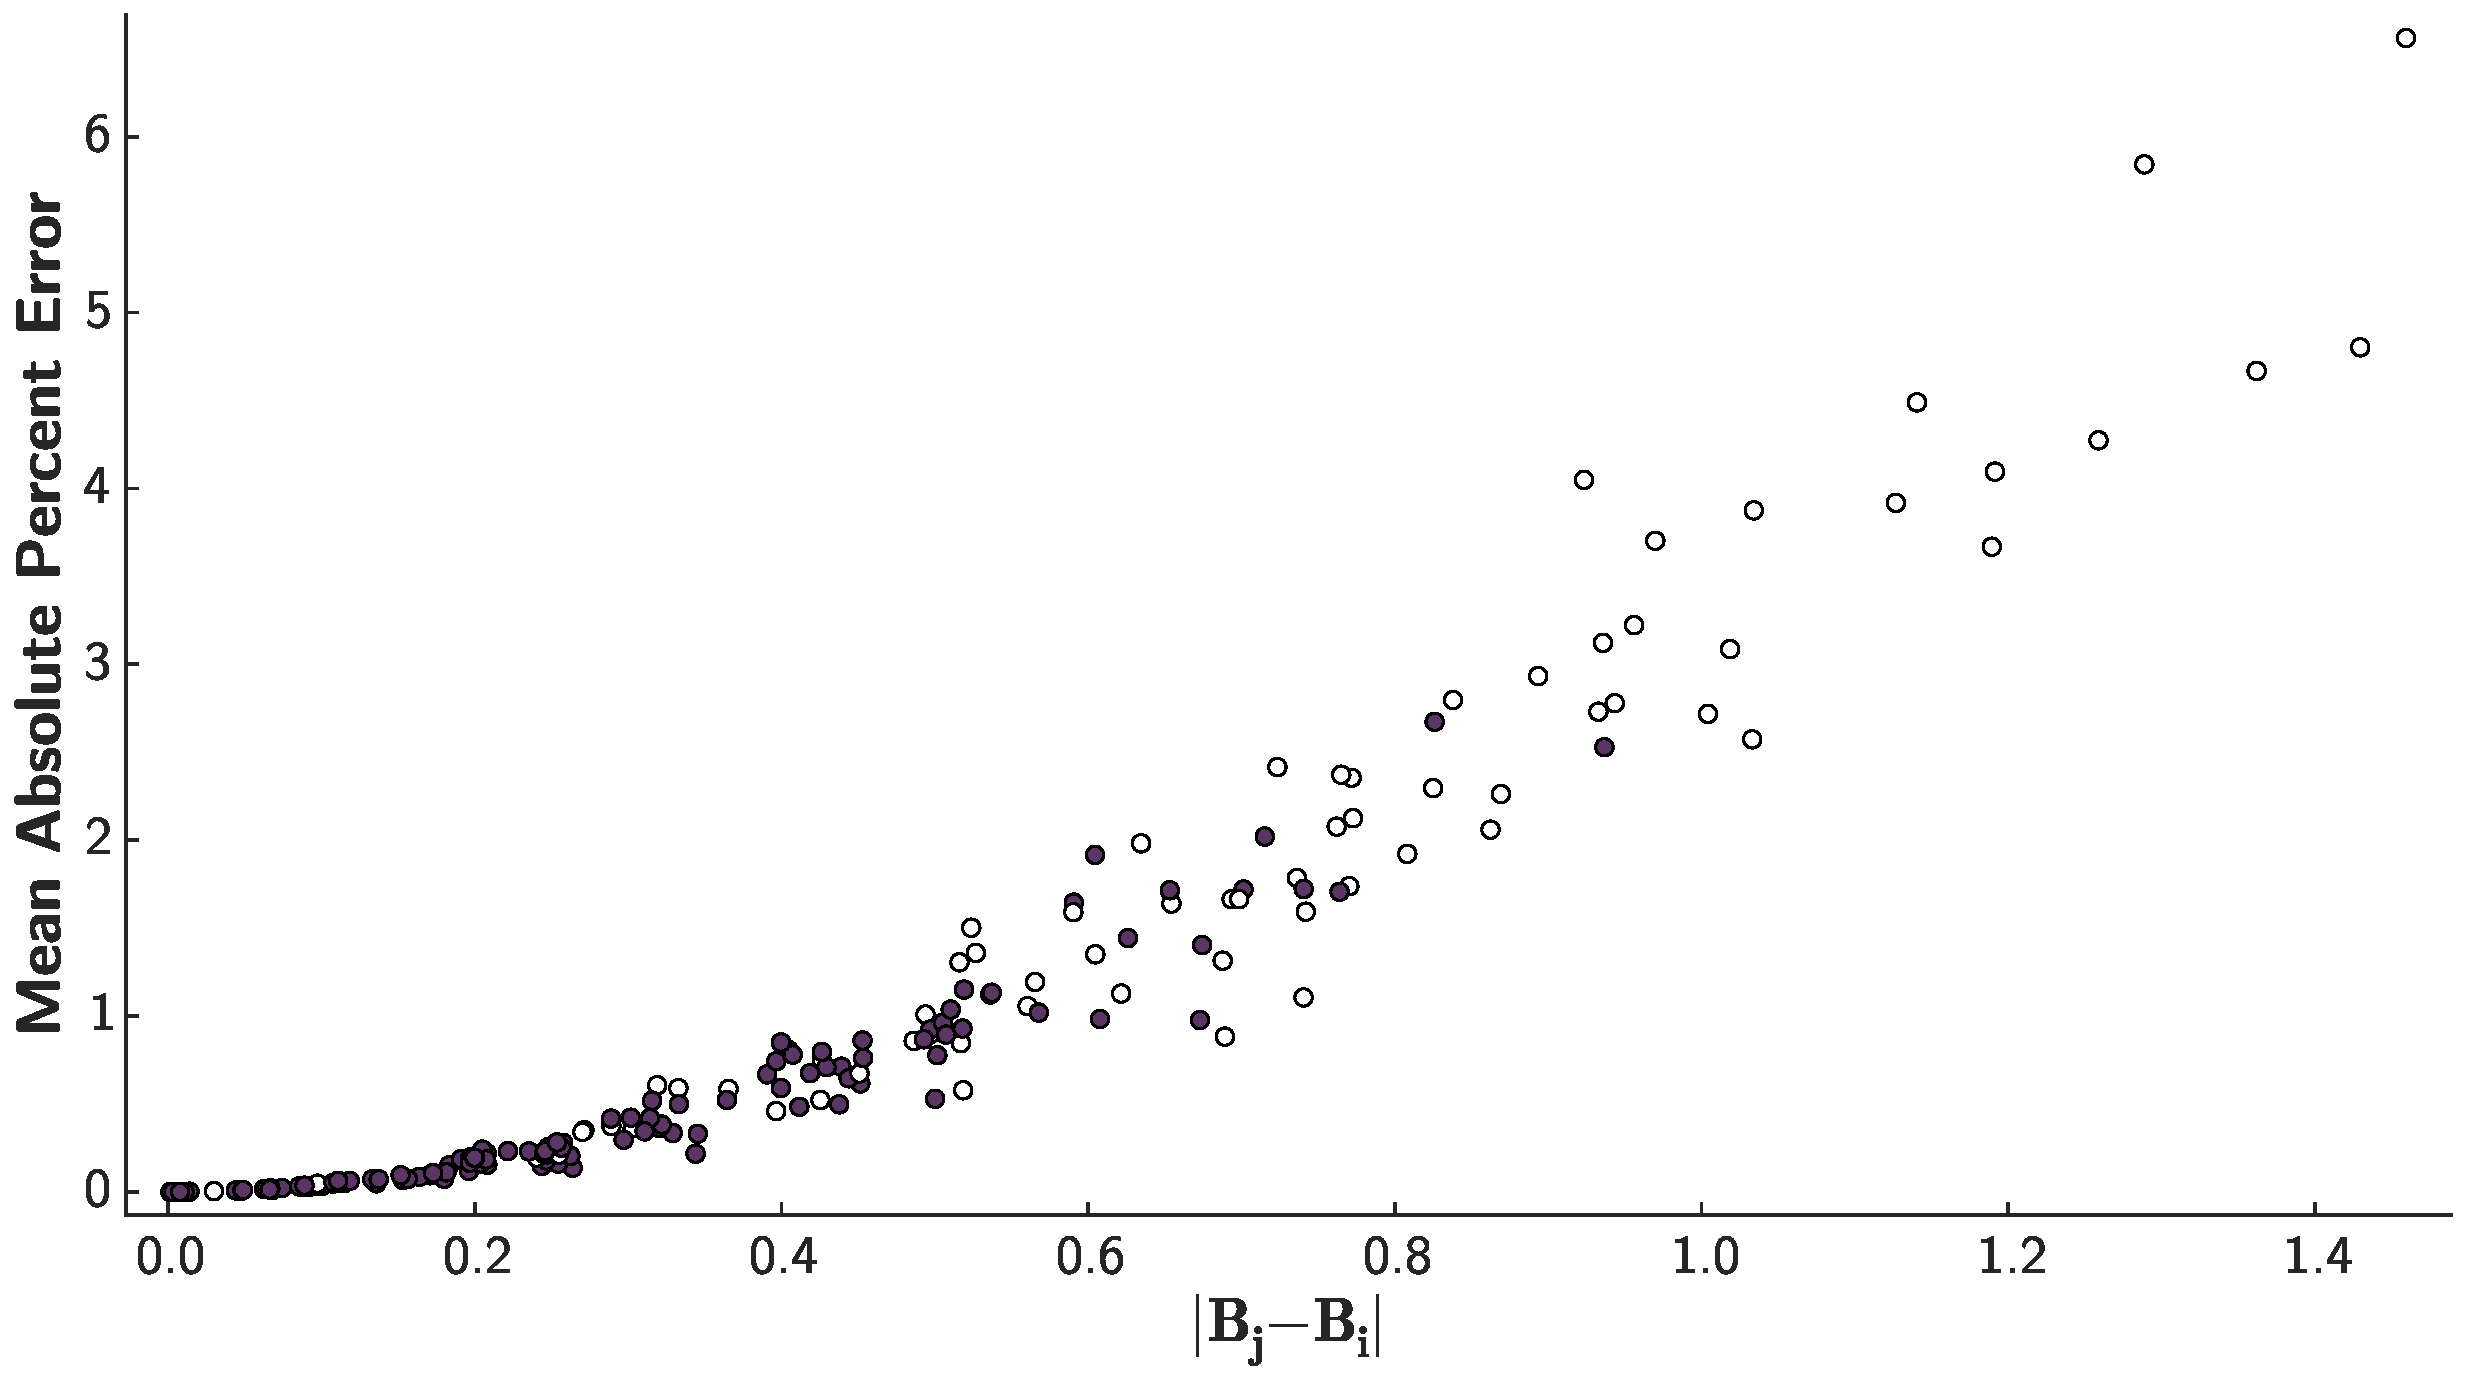
\includegraphics[width=0.9\textwidth]{isotropic/si/bij_mape.pdf}
    \caption{
        Mean absolute percent error of fitted overlap values as a function of the
        absolute difference between $B_i$ and $B_j$ values. Element pairs containing
        He, Li, Ne and/or Na are shown as empty circles.  Deviations below 1\% are
        seen for most element pairs, with noble gases and alkali metals posing a more
        significant challenge. Scatter in the plot is due to small variations in the
        absolute values of \R fit for each pair.  As expected, \sijexact and
        \sijapprox closely agree for $|B_i - B_j| \approx 0$. 
           		  }
    \label{fig:bij_mape}
    \end{figure}
    %%%%%%%%%%%%%%% Bij MAPE %%%%%%%%%%%%%%%%%

Relative errors for fitting are acceptably small for all element pairs.
Excluding certain noble gases and alkali metals (He, Li, Ne,
Na) from consideration, these being the elements with the most disparate $B_i$
values compared to other elements, MAPE drops below 3\% for all pairs, with
the vast majority of MAPE below 1\%. Our focus in this work is primarily on
organic compounds where $|B_i - B_j|$ is small; empirically, these errors always translate to very small
errors in the exchange energy itself.  
Use of an effective \B may require further testing in cases with extremely
disparate $B_i$ and $B_j$ values.

We next tested whether the optimized \B could instead be modeled by
a combination rule $\B = f(B_i,B_j)$.  On the basis of symmetry and scaling
considerations, \citeauthor{Waldman1993} demonstrate that if a
combination rule $f(B_i,B_j)$ exists, a plot of $\sfrac{\B}{B_i}$ vs.
$\sfrac{B_j}{B_i}$ should lie on a single curve.\cite{Waldman1993} Remarkably
(see \ref{fig:bij_combination_rule}), a geometric mean combination rule $\B =
\sqrt{B_iB_j}$ models the fitted \B values near quantitatively. This
result allows the computation of Slater overlaps
using the much simpler
form of \sijapprox (\ref{eq:simple_overlap}) 
from individual atoms-in-molecule exponents $B_i$ and $B_j$.

    %%%%%%%%% Bij Combination Rule %%%%%%%%%%%
    \begin{figure}[t]
    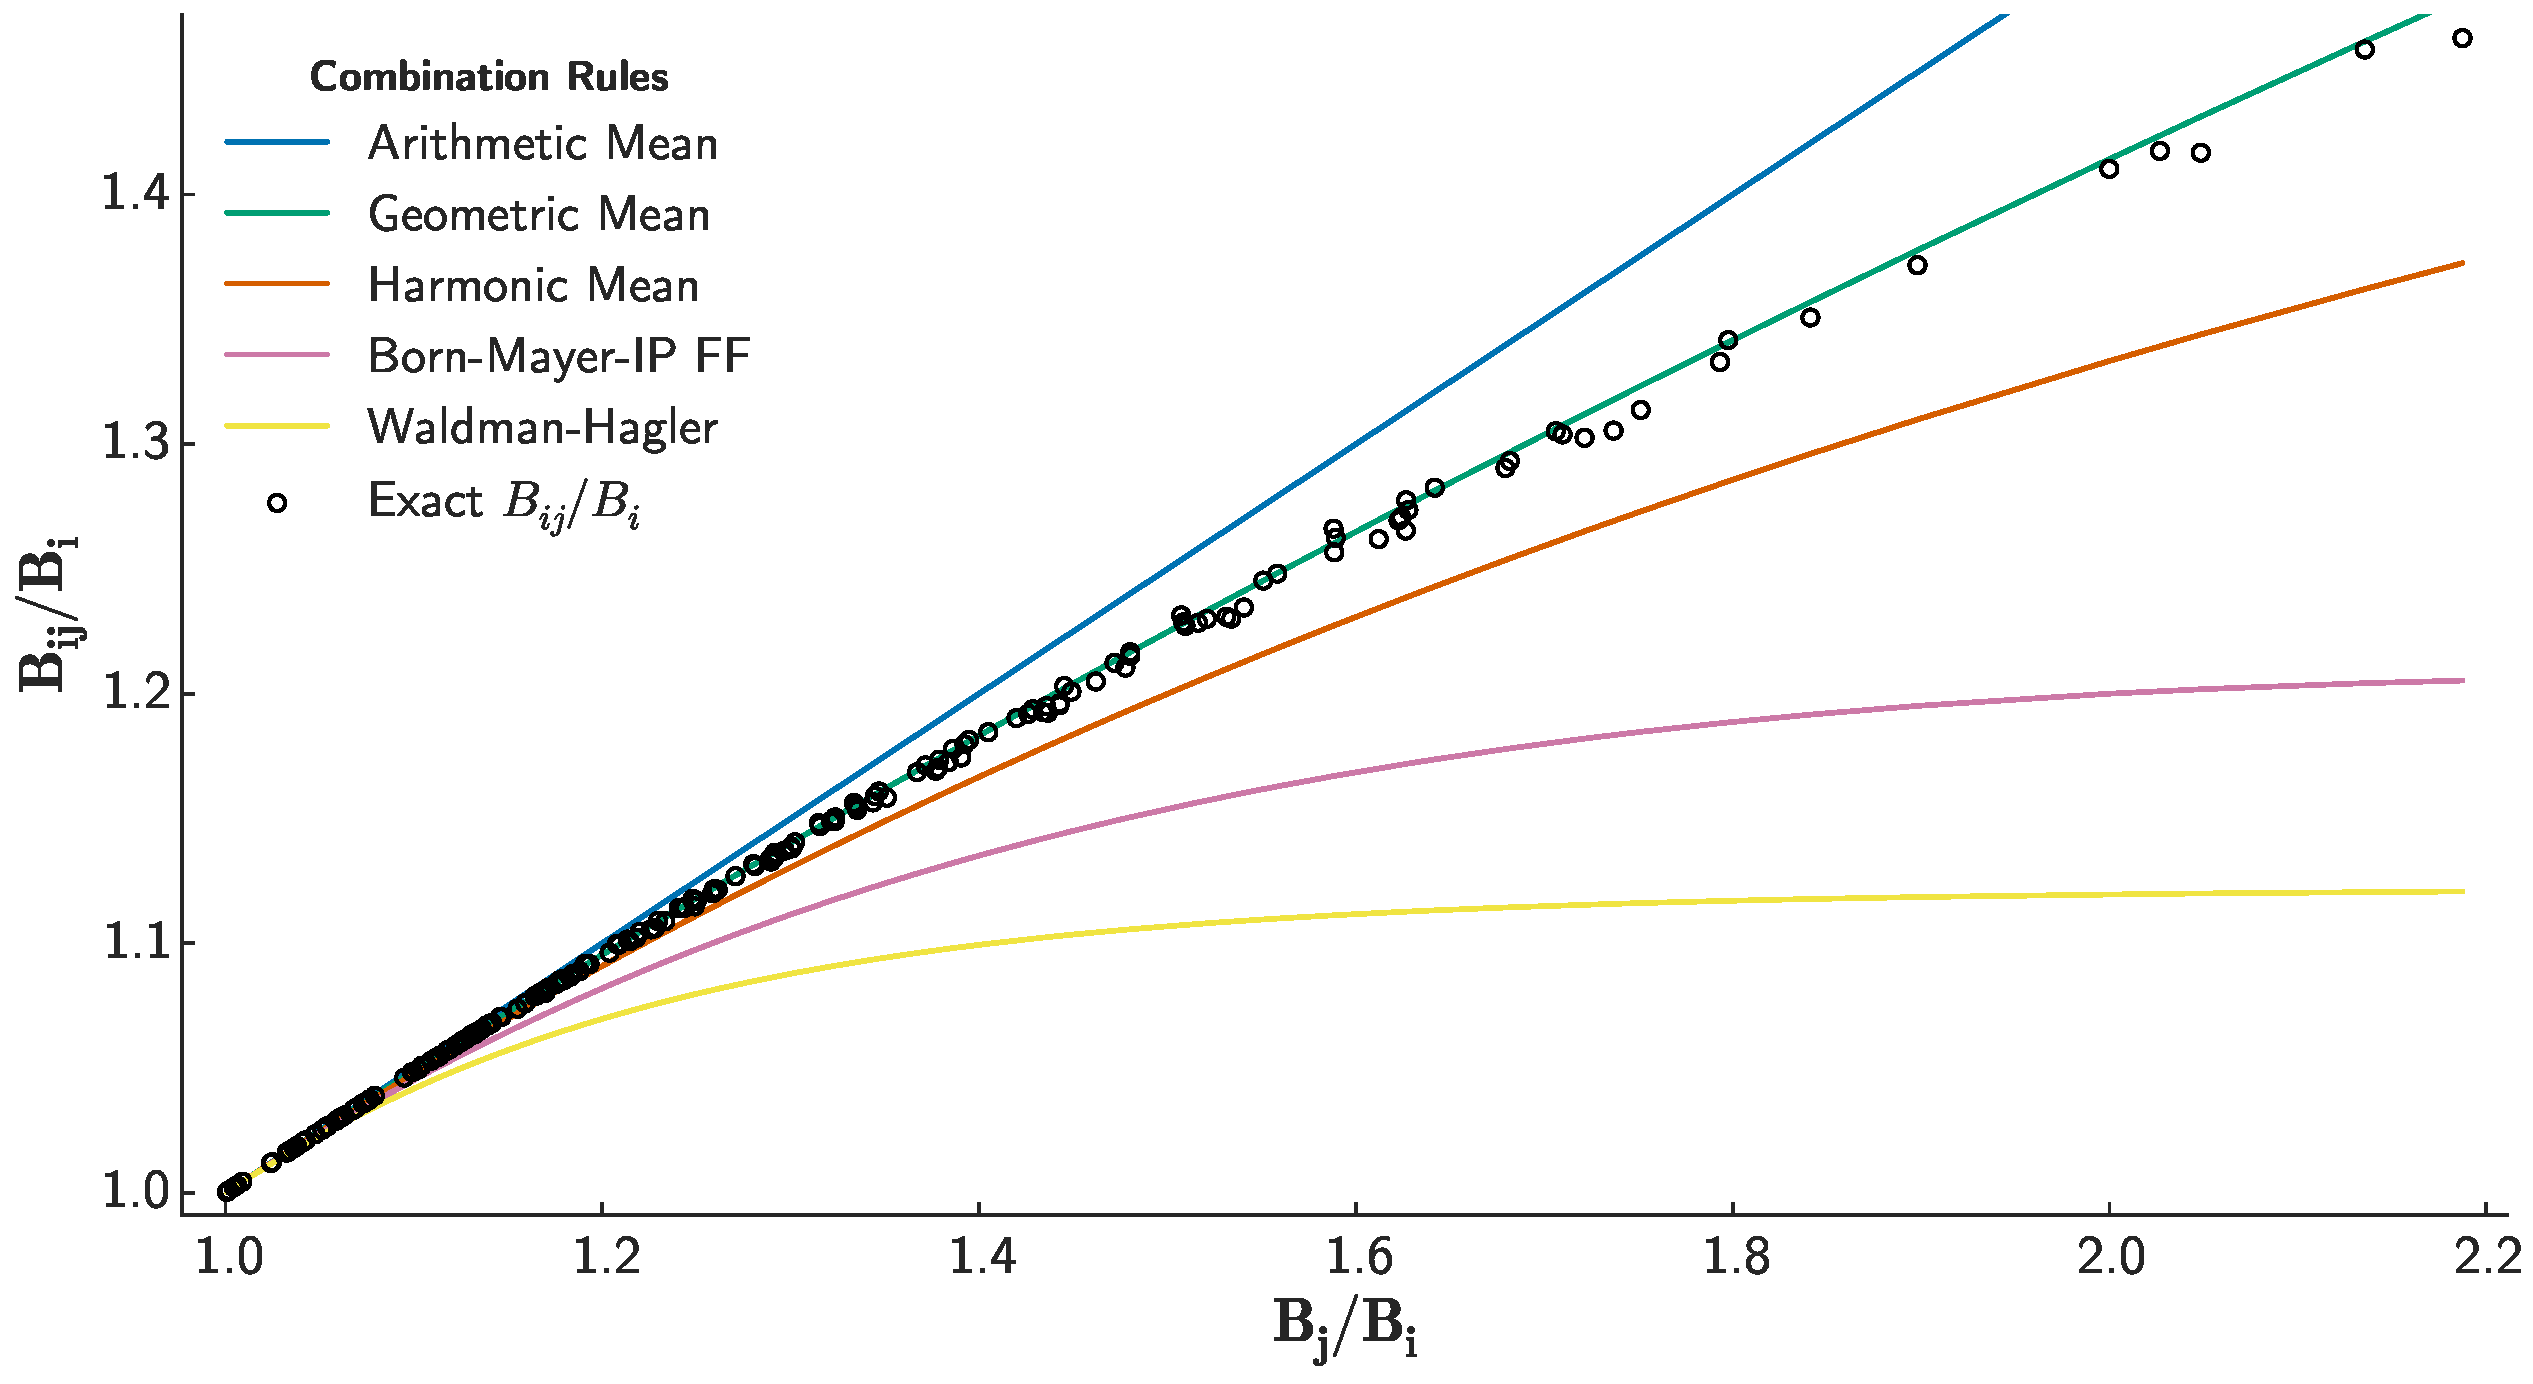
\includegraphics[width=0.9\textwidth]{isotropic/si/bij_combination_rule.pdf}
    \caption{
    Waldman-Hagler-style analsysis of possible $B_{ij}$ combination rules.  Exact
    $B_{ij}$ values are derived from fitting an approximate overlap density of the form $S_{ij}
    = A_{ij} K_2(r_{ij})\exp(-B_{ij}r_{ij})$ to the exact overlap density (as given by Rosen
    and by Tai\cite{Rosen1931,Tai1986}) of two distinct Slater orbitals whose exponents
    correspond to atomic exponents for the elements H-Ar, Cl, Br, and I. For each overlap pair,
    a range of \R values was used from 0.8 to 1.2 times the sum of the pair's van der Waals radii.
    The geometric mean combination rule $B_{ij} = \sqrt{B_iB_j}$ models the exact $B_{ij}$
    values with near-perfect agreement, justifying our choice of combination rule.
           		  }
    \label{fig:bij_combination_rule}        
    \end{figure}
    %%%%%%%%% Bij Combination Rule %%%%%%%%%%%

\end{section}
%% \begin{section}{Force Field Fit Quality: Exact Overlap Model vs. \isaffold}
%% 
%% 
%% A direct test of the approximate overlap model (Equation
%% \ref{eq:simple_overlap} with $B_i$ values extracted from ISA calculations,
%% synonymous with the \isaffold in the main text) is
%% made by directly comparing the accuracy of force fields fit by the exact and
%% approximate overlap models.
%% \ref{tab:rmse_comparison} shows average RMS errors for each energy component
%% that uses an explicit short-range term. 
%% Differences in RMS errors between models are
%% negligible, with use of the more approximate overlap model introducing (at
%% most) an additional 2\% extra error compared to the exact overlap model. 
%% Use of \sijapprox to compute all overlaps is thus
%% well justified.
%% 
%% \begin{table}
%% \centering
%% \renewcommand\arraystretch{1.1}
%% \begin{tabular}{@{}rcccc@{}}
%% \hline
%% \toprule
%% \multirow{2}{*}{Component} & &  \isaffold & Exact Overlap Model & \multirow{2}{*}{$\alpha$}  \\
%%      & & \multicolumn{1}{c}{(kJ mol$^{-1}$)}& \multicolumn{1}{c}{(kJ mol$^{-1}$)} &  \\
%% \midrule
%% Exchange        & &    2.641  (0.686)  &  2.581  (0.679) &  1.023 (1.010) \\
%% Electrostatics  & &    1.087  (0.351)  &  1.083  (0.350) &  1.004 (1.003) \\
%% Induction       & &    0.251  (0.095)  &  0.252  (0.095) &  0.998 (0.999) \\
%% \dhf            & &    0.246  (0.068)  &  0.245  (0.068) &  1.004 (1.007) \\
%% \bottomrule
%% \hline
%% \end{tabular}
%% \caption{
%%     Comparison of geometric mean RMS errors over the 91 dimer test
%%     set for the Approximate Overlap Model (that is, the \isaffold) and the
%%     Exact Overlap Model.  `Attractive' RMS errors, representing the average RMS
%%     error for the subset of points whose energies are net attractive ($\etot < 0$), 
%%     are shown in parentheses to the right of the total average RMS errors.
%%     The average ratio of RMS errors (\isaffold / Exact Overlap Model) for each pair in
%%     the 91 dimer test set, $\alpha$ (dimensionless), is also shown. $\alpha$
%%     values greater than 1 indicate that on average the Exact Overlap Model is more
%%     accurate compared to the \isaffold.
%% 	}
%% \label{tab:rmse_comparison}
%% \end{table}
%% 
%% 
%% \end{section}
%% \clearpage
%% \begin{section}{Extrapolation Algorithm for ISA Exponents}
%% 
%% Unphysical asymptotic charge density decays occasionally arise in the ISA
%% procedure due to basis set incompleteness and numerical instabilities. These
%% unphysical decays can
%% skew optimization of $B_i^{ISA}$ parameters, and need to be corrected.
%% Generally speaking, there exists some range of distances in the valence region
%% that \emph{does} exhibit the expected exponential decay; we extrapolate the
%% decay from this intermediate region to describe the asymptotic region using
%% the following algorithm:
%% 
%% \begin{enumerate}
%% 
%% \item Take the log of each atomic density (henceforth logdens) to linearize
%% the asymptotic density.
%% \label{step1}
%% \item Compute the 2\super{nd} derivative of logdens. This can be
%% done analytically, as the \isa procedure outputs an analytical expression (in
%% terms of Gaussian basis functions) for the atomic density.
%% \label{step2}
%% \item Determine the `intermediate region' of exponential decay by locating the
%% largest range where the 2\super{nd} derivative of logdens is zero
%% to within a fixed tolerance.  Here we utilize a tolerance of 0.3 a.u. (absolute cutoff)
%% or 190\% of the smallest exponent in the Gaussian basis set (relative cutoff),
%% whichever is smaller.  
%% The latter cutoff accounts for the eventual asymptotic Gaussian-type decay
%% dictated by the smallest $\zeta$ in the ISA basis.
%% The endpoints of this intermediate region are denoted $r1$ and $r2$, respectively.
%% \item Calculate the slope $m$ and intercept $b$ for the line defined by
%% $r1$, $r2$, and their respective values of logdens. 
%% \label{step3}
%% \item Replace all values of logdens after $r2$ with $mr + b$.  The resulting
%% atomic density is labeled in the main text as `Asymptotically-corrected ISA
%% densities'.
%% \label{step4}
%% 
%% \end{enumerate}
%% 
%% A visual of these steps is shown in \ref{fig:acetone-extrapolation}.
%% 
%% 
%%     %%%%%%%%% Bij Combination Rule %%%%%%%%%%%
%%     \begin{figure}
%%     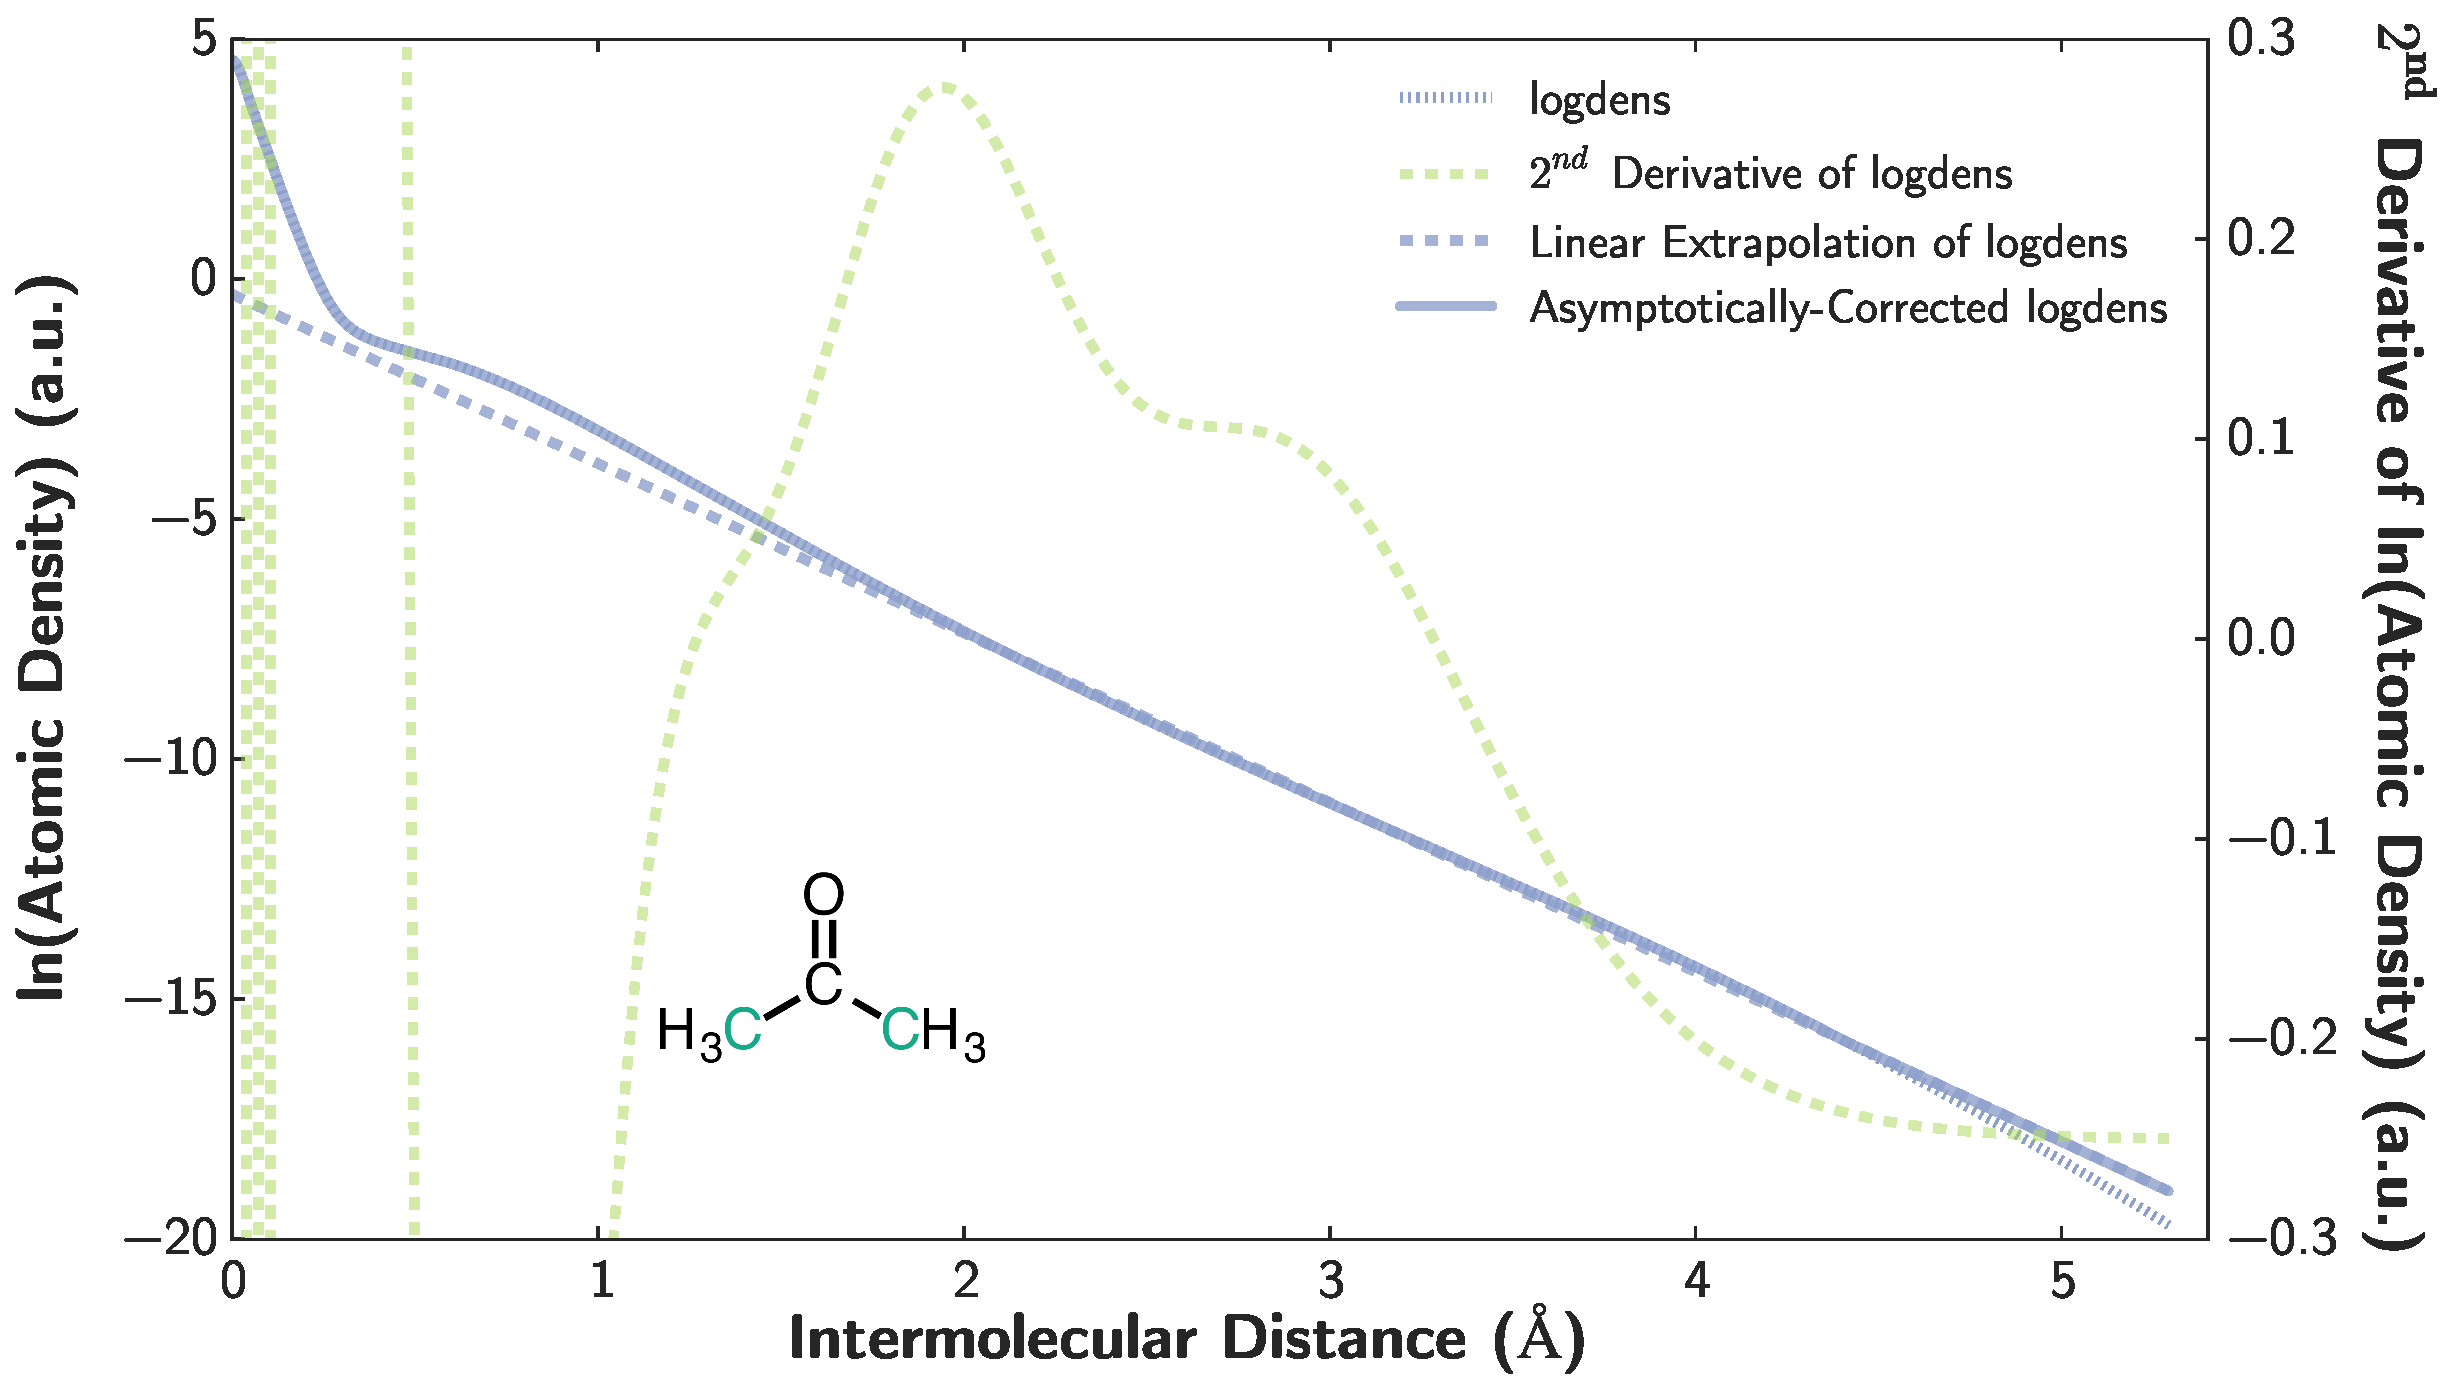
\includegraphics[width=0.9\textwidth]{isotropic/si/acetone_extrapolation.pdf}
%%     \caption{
%%         Linear extrapolation algorithm for the methyl carbon in acetone.
%% Depicted are (in legend order) Steps \ref{step1}, \ref{step2}, \ref{step3},
%% and \ref{step4} in the extrapolation algorithm. Note that some portions of the
%% $2^{nd}$ derivative extend off the graph; also note that most of logdens
%% is located underneath the asymptotically-corrected curve.
%%            		  }
%%     \label{fig:acetone-extrapolation}        
%%     \end{figure}
%%     %%%%%%%%% Bij Combination Rule %%%%%%%%%%%
%% 
%% 
%% 
%% \end{section}
%% \clearpage
%% \begin{section}{Non-polarizable, point-charge Lennard-Jones Force Fields}
%% 
%% As described in the main text, a non-polarizable, rank 0 multipole version of
%% \ljff was fit in order to produce force fields most in line with popular
%% standard force fields. Results for this \ljff are shown in
%% \tabref{tab:lj_rmse}; unsurprisingly, these force fields are less accurate and
%% less transferable compared to \ljff in the main text, which includes
%% polarizability and higher-order multipole moments.
%% 
%% 
%% %%%%%%%%%%%%%%%%%%%%% Average LJ RMSE Table %%%%%%%%%%%%%%%%%%%%%%%%%%%%%%%%%%%
%% %\begin{landscape}
%% \begin{table}
%% \small
%% \centering
%% \renewcommand\arraystretch{1.1}
%% \begin{tabular}{@{}rcccc@{}}
%% \hline
%% \toprule
%% & \phantom{} &
%%   \multicolumn{1}{c}{Dimer-Specific Fits} &
%%   \phantom{ab} &
%%   \multicolumn{1}{c}{Transferable Fits} \\
%% %\cmidrule{2} \cmidrule{3}
%% 
%% %% Component & & \ljff-q0, $\lambda=0.1$ & \ljff-q2, $\lambda=0.1$ & \ljff-q2, $\lambda=2.0$ 
%% %%           & & \ljff-q0, $\lambda=0.1$ & \ljff-q2, $\lambda=0.1$ & \ljff-q2, $\lambda=2.0$ \\
%% %%           & & \ljff-q2,               & \ljff-q2,               & \ljff-q0,               
%% %%           & & \ljff-q2,               & \ljff-q2,               & \ljff-q0,               \\
%% %%           & &           $\lambda=2.0$ &           $\lambda=0.1$ &           $\lambda=0.1$ 
%% %%           & &           $\lambda=2.0$ &           $\lambda=0.1$ &           $\lambda=0.1$ \\
%%      & & \multicolumn{1}{c}{(kJ mol$^{-1}$)} 
%%      & & \multicolumn{1}{c}{(kJ mol$^{-1}$)} \\
%% \midrule
%% %\addlinespace
%% %\textbf{
%% %Total Energy}   \\
%% %\emph{RMSE}             & &  1.984 (0.603)   &  6.058 (0.413)  &  5.116 (0.560)   && 2.054 (0.640)  &  5.760 (0.457)  &  4.513 (0.658) \\
%% \emph{RMSE}             & &    5.116 (0.560)   &&   4.513 (0.658) \\
%% %\addlinespace
%% \emph{\mse}
%%                  %& &  0.322 (0.345)   &  1.610 (0.041)  &  0.803 (0.038)   && 0.311 (0.368)  &  1.410 (0.060)  &  0.562 (0.079) \\
%%                  & &    0.803 (0.038)   &&   0.562 (0.079) \\
%% \bottomrule
%% \hline
%% \end{tabular}
%% \caption{
%%     Comparison of characteristic RMSE and \mse over the 91 dimer test
%%     set for the non-polarizable, rank 0 multipole Lennard-Jones model. The LJ
%%     models are not parameterized on a component-by-component basis, thus
%%     RMSE/\mse values for only the total FF energy is shown.  `Attractive'
%%     errors, representing the average RMSE/\mse for the subset of points
%%     whose energies are net attractive ($\etot < 0$), are shown in parentheses to
%%     the right of the total average RMS errors. `Dimer-Specific Fits' and
%%     `Transferable Fits' are as in the main text.
%% 	}
%% \label{tab:lj_rmse}
%% \end{table}
%% \normalsize
%% %\end{landscape}
%% %%%%%%%%%%%%%%%%%%%%% Average LJ RMSE Table %%%%%%%%%%%%%%%%%%%%%%%%%%%%%%%%%%%
%% 
%% 
%% \end{section}
%% \begin{section}{Born-Mayer-sISA: Scale Factor Tests}
%% 
%% \begin{subsection}{Comparison to $S_{ij}$}
%% 
%% Exact $S_{ij}$ (\eqref{eq:simple_overlap} and \eqref{eq:complicated_overlap})
%% values were computed for various element pairs as in
%% \secref{sec:bij_combo_rule}. Born-Mayer overlaps of the form
%% %
%% \begin{align*}
%% S_{ij} &\approx K_{ij}\exp(-\xi B_{ij} \R) \\
%% \intertext{where}
%% K_{ij} &= \frac{K}{B^{3}_{ij}} \\
%% B_{ij} &= \sqrt{B_i B_j}
%% \end{align*}
%% %
%% were fit to these exact overlaps; $K$ and $\xi$ were optimized as universal
%% parameters by performing a log-weighted fit over the entire set of $S_{ij}$
%% values. 
%% 
%% %%%%%%%%%%%%%%%%%%%%% Optimized S_IJ parameters Table %%%%%%%%%%%%%%%%%%%%%%%%%%%%%%%%%%%
%% \begin{table}
%% \small
%% \centering
%% \renewcommand\arraystretch{1.1}
%% \begin{tabular}{@{}rcccc@{}}
%% \hline
%% \toprule
%% Range of \R & \phantom{ab} & $\xi$ & \phantom{ab} & K \\
%% %% \multicolumn{5}{l}{(Fraction of Van der Waals radii for each atom pair)} \\
%% \midrule
%% {$[0.8,1.2]$} & & 0.738   & & 12.2  \\
%% {$[1.0,2.0]$} & & 0.812   & & 20.9  \\
%% {$[1.0,4.0]$} & & 0.878   & & 42.6  \\ 
%% 
%% \bottomrule
%% \hline
%% \end{tabular}
%% \caption{
%%     Optimized Born-Mayer parameters, $\xi$ and $K$, for fits to \\
%% $S_{ij} \approx \frac{K}{(B_iB_j)^{\sfrac32}}\exp(-\xi \sqrt{B_iB_j} \R)$.
%% $B_i$ and $B_j$ values have been chosen as in \ref{sec:bij_combo_rule}.
%% Tabulated \R ranges are expressed as a fraction of the sum of van der Waals
%% radii for atoms $i$ and $j$.
%% 	}
%% \label{tab:sij_scale_factor}
%% \end{table}
%% \normalsize
%% %%%%%%%%%%%%%%%%%%%%% Optimized S_IJ parameters Table %%%%%%%%%%%%%%%%%%%%%%%%%%%%%%%%%%%
%% 
%% Optimized parameters are shown in \ref{tab:sij_scale_factor} for various
%% ranges of \R.
%% As shown in
%% \ref{tab:sij_scale_factor}, the scale factor $\xi$ is highly sensitive to
%% the values of \R included in the fits, with larger values of \R tending to
%% increase $\xi$. On the other hand, $\xi$ is fairly insensitive to the
%% values of $B_i$ and $B_j$: setting $\xi = \xi_0 + \xi_1 B_{ij}$ does
%% not significantly improve fit quality. On the grounds of our overlap
%% tests, it is difficult to establish a precise value for $\xi$, though our
%% results do suggest that $\xi \sim 0.80$ and is largely independent of
%% the atomic exponents themselves.
%% 
%% \end{subsection}
%% \begin{subsection}{Comparison to \vtot}
%% 
%% Alternatively, we
%% optimized the \bmsisaff scale factor by minimizing errors in the force field 
%% itself. Average RMS errors for a variety of scale factors are shown in
%% \ref{tab:bmsisaff_scale_rmse}. Regardless of whether we consider each energy
%% component separately, or focus on the overall energy, setting $\xi=0.84$
%% is optimal; RMS errors for this choice are
%% comparable to the \isaffold itself.
%% 
%% %%%%%%%%%%%%%%%%%%%%% Average RMSE Table %%%%%%%%%%%%%%%%%%%%%%%%%%%%%%%%%%%
%% \begin{landscape}
%% \begin{table}
%% \small
%% \centering
%% \renewcommand\arraystretch{1.1}
%% \begin{tabular}{@{}rccccccc@{}}
%% \hline
%% \toprule
%% & \phantom{ab} &
%%   \multicolumn{6}{c}{Born-Mayer-sISA Scale Factor} 
%%   \\
%% \cmidrule{3-8}
%% 
%% Component & & $\xi= 0.80$ & $\xi= 0.82$ & $\xi= 0.84$ & $\xi= 0.86$ & $\xi = 0.88$ & $\xi = 0.90$  \\
%%      %% & & \multicolumn{1}{c}{(kJ mol$^{-1}$)} & \multicolumn{1}{c}{(kJ mol$^{-1}$)} &  \multicolumn{1}{c}{(kJ mol$^{-1}$)}
%%      %% & & \multicolumn{1}{c}{(kJ mol$^{-1}$)}& \multicolumn{1}{c}{(kJ mol$^{-1}$)} \\
%% \midrule
%% Exchange        & &  3.078 (0.697)   &    2.690 (0.668) &  2.677 (0.686)  & 2.841 (0.702)  &    3.225 (0.742)  &    3.798 (0.791) \\
%% Electrostatics  & &  1.144 (0.418)   &    1.105 (0.378) &  1.083 (0.352)  &    1.077 (0.342)  &    1.104 (0.354)  &    1.105 (0.373)  \\
%% Induction       & &  0.258 (0.099)   &    0.253 (0.097) &  0.250 (0.096)  &    0.246 (0.095)  &    0.243 (0.094)  &    0.240 (0.094)  \\
%% \dhf            & &  0.241 (0.072)   &    0.244 (0.069) &  0.248 (0.068)  &    0.255 (0.070)  &    0.263 (0.075)  &    0.272 (0.082)  \\
%% Dispersion      & &  0.934 (0.383)   &    0.803 (0.337) &  0.856 (0.336)  &    1.078 (0.370)  &    1.388 (0.426)  &    1.740 (0.496)  \\
%% \addlinespace                                                                                                                        
%% \textbf{                                                                                                                             
%% Total Energy}   & &  1.970 (0.503)   &    1.775 (0.455) &  1.751 (0.453)  &    1.818 (0.465)  &    2.084 (0.516)  &    2.451 (0.577) \\
%% \bottomrule
%% 
%% 
%% \hline
%% \end{tabular}
%% \caption{
%% 	Average RMS errors over the 91 dimer test set for \bmsisaff using different exponential scale factors. 
%% 	All quantities are in kJ mol$^{-1}$ except for scale factors, which are unitless.
%%     `Attractive' RMS errors, representing the average RMS error for
%%     the subset of points whose energies are net attractive (i.e., where $E_{tot} <
%%     0$), are shown in parentheses to the right of the total average RMS errors.
%%     Geometric (rather than arithmetic) averages are used in all cases.
%% 	}
%% \label{tab:bmsisaff_scale_rmse}
%% \end{table}
%% \normalsize
%% \end{landscape}
%% %%%%%%%%%%%%%%%%%%%%% Average RMSE Table %%%%%%%%%%%%%%%%%%%%%%%%%%%%%%%%%%%
%% 
%% \end{subsection}
%% 
%% \end{section}
%% \begin{section}{Slater-OPT and Born-Mayer-OPT Force Fields}
%% 
%% We developed a Slater-OPT force field,
%% identical to the \isaffold except that \B parameters were optimized to reproduce the
%% DFT-SAPT exchange-repulsion energy.
%% Analogously, we developed Born-Mayer-OPT as an
%% extension of the \bmsisaff. Treating \B as a completely
%% unconstrained parameter led to poor dispersion energies and overall
%% transferability, and was not considered further.
%% Instead, exponents were optimized using a harmonic
%% penalty function of the form $k(B-B_0)^2$, with $k=10^{-5}$ a.u.  For
%% Slater-OPT, $B_0$ values were taken from the \isaffold; for Born-Mayer-OPT, the \saptff
%% values were used. 
%% RMS errors for Slater-OPT and Born-Mayer-OPT are shown in
%% \ref{tab:bmopt_rmse}. 
%% For both Dimer-Specific and Transferable fits, Slater-OPT and Born-Mayer-OPT are
%% of comparable quality. Both force fields are only slight improvements to
%% either the \isaffold or the \bmsisaff; considering the extra number of free parameters
%% required to optimize atomic exponents, we consider these results further
%% confirmation of the inherent quality of the ISA exponents.
%% 
%% %%%%%%%%%%%%%%%%%%%%% Average RMSE Table %%%%%%%%%%%%%%%%%%%%%%%%%%%%%%%%%%%
%% %\begin{landscape}
%% \begin{table}
%% \small
%% \centering
%% \renewcommand\arraystretch{1.1}
%% \begin{tabular}{@{}rcccccc@{}}
%% \hline
%% \toprule
%% & \phantom{ab} &
%%   \multicolumn{2}{c}{Dimer-Specific Fits} &
%%   \phantom{ab} &
%%   \multicolumn{2}{c}{Transferable Fits} \\
%% \cmidrule{3-4} \cmidrule{6-7}
%% 
%% Component & & Slater-OPT & Born-Mayer-OPT & & Slater-OPT & Born-Mayer-OPT  \\
%%      & & \multicolumn{1}{c}{(kJ mol$^{-1}$)}  &  \multicolumn{1}{c}{(kJ mol$^{-1}$)}
%%      & & \multicolumn{1}{c}{(kJ mol$^{-1}$)}  &  \multicolumn{1}{c}{(kJ mol$^{-1}$)} \\
%% \midrule
%% Exchange        & &    2.513 (0.636)   &    2.433 (0.639)  & &    2.507 (0.665)  &   2.459 (0.671) \\
%% Electrostatics  & &    1.087 (0.362)   &    1.068 (0.352)  & &    1.129 (0.359)  &   1.113 (0.352) \\
%% Induction       & &    0.256 (0.097)   &    0.252 (0.096)  & &    0.282 (0.102)  &   0.280 (0.102) \\
%% \dhf            & &    0.241 (0.068)   &    0.244 (0.067)  & &    0.272 (0.077)  &   0.276 (0.077) \\
%% Dispersion      & &    0.836 (0.330)   &    0.822 (0.349)  & &    0.823 (0.331)  &   0.820 (0.350) \\
%% \addlinespace                                                                        
%% \textbf{                                                                
%% Total Energy}  \\ 
%% \emph{RMSE}
%%                 & &    1.549 (0.448)   &    1.597 (0.450)  & &    1.482 (0.454)  &   1.532 (0.458) \\
%% \emph{\mse}
%%                 & &    0.160 (0.065)   &    0.160 (0.084)  & &    0.149 (0.057)  &   0.204 (0.130) \\
%% \bottomrule
%% 
%% \hline
%% \end{tabular}
%% \caption{
%%     Comparison of geometric mean RMS errors over the 91 dimer test
%%     set for the Slater-OPT and Born-Mayer-OPT methods.
%%     `Attractive' RMS errors, representing the average RMS
%%     error for the subset of points whose energies are net attractive ($\etot < 0$), 
%%     are shown in parentheses to the right of the total average RMS errors.
%% 	}
%% \label{tab:bmopt_rmse}
%% \end{table}
%% \normalsize
%% %\end{landscape}
%% %%%%%%%%%%%%%%%%%%%%% Average RMSE Table %%%%%%%%%%%%%%%%%%%%%%%%%%%%%%%%%%%
%% 
%% 
%% 
%% 
%% \end{section}
%% 
%% 
%% \begin{section}{Monomer Geometries}
%% 
%% Geometries for each molecule in the 91 dimer test set are listed below, in
%% alphabetical order. Also listed are the relevant energies (highest occupied
%% molecular orbital and ionization potential) for the asymptotic correction
%% required in DFT-SAPT calculations of each molecule. All asymptotic corrections
%% were performed at a PBE0/\avtz level of theory. Distances and energies are in
%% a.u.
%% 
%% \scriptsize
%% \centering
\renewcommand\arraystretch{1.1}
\newcolumntype{L}{D{.}{.}{2,6}}
\begin{longtable}{@{}rLLL@{}}
\caption{Cartesian coordinates for each molecule in the 91 dimer test set. HOMO
and I.P. values, necessary for DFT-SAPT calculations, are also shown. All units
are in a.u.}
\label{tab:geometries}
\\

\endfirsthead

\multicolumn{4}{c}%
{{\bfseries \tablename\ \thetable{} -- continued from previous page}} \\
\hline
\endhead
%% \toprule
%% Atomtype & 
%% \multicolumn{1}{c}{$Q_{00 }$} &
%% \multicolumn{1}{c}{$Q_{10 }$} &
%% \multicolumn{1}{c}{$Q_{11c}$} &
%% \multicolumn{1}{c}{$Q_{11s}$} &
%% \multicolumn{1}{c}{$Q_{20 }$} &
%% \multicolumn{1}{c}{$Q_{21c}$} &
%% \multicolumn{1}{c}{$Q_{21s}$} &
%% \multicolumn{1}{c}{$Q_{22c}$} &
%% \multicolumn{1}{c}{$Q_{22s}$} \\
%% \midrule
%% \endhead
%% 
%% \bottomrule
%% \endfoot

\multicolumn{4}{l}{\textbf{Acetone}}  \\*
\toprule
C      &   0.000000  &   0.000000  &  -2.280333 \\* 
O      &   0.000000  &   0.000000  &   0.000000 \\* 
C      &   0.000000  &   2.435101  &  -3.793814 \\* 
C      &   0.000000  &  -2.435101  &  -3.793814 \\* 
H      &   0.000000  &   4.050439  &  -2.525430 \\* 
H      &   0.000000  &  -4.050439  &  -2.525430 \\* 
H      &   1.657668  &   2.514281  &  -5.019869 \\* 
H      &  -1.657668  &   2.514281  &  -5.019869 \\* 
H      &  -1.657668  &  -2.514281  &  -5.019869 \\* 
H      &   1.657668  &  -2.514281  &  -5.019869 \\* 

\bottomrule
\multicolumn{2}{l}{HOMO:} &
-0.266741       
\\*
\multicolumn{2}{l}{I.P.:} &
0.35386979
\\*
\\

\multicolumn{4}{l}{\textbf{Ar}}  \\*
\toprule
Ar     &   0.000000  &   0.000000  &   0.000000 \\* 

\bottomrule
\multicolumn{2}{l}{HOMO:} &
-0.440599       
\\*
\multicolumn{2}{l}{I.P.:} &
0.58049447
\\*
\\

\multicolumn{4}{l}{\textbf{Chloromethane}}  \\*
\toprule
C      &   0.000000  &   0.000000  &  -3.365602 \\* 
Cl     &   0.000000  &   0.000000  &   0.000000 \\* 
H      &   1.969851  &   0.000000  &  -4.102784 \\* 
H      &  -0.984925  &   1.705856  &  -4.102784 \\* 
H      &  -0.984925  &  -1.705856  &  -4.102784 \\* 

\bottomrule
\multicolumn{2}{l}{HOMO:} &
-0.313074       
\\*
\multicolumn{2}{l}{I.P.:} &
0.41507894
\\*
\\

\multicolumn{4}{l}{\textbf{CO\sub2}}  \\*
\toprule
C      &   0.000000  &   0.000000  &   0.000000 \\* 
O      &   0.000000  &   0.000000  &   2.196051 \\* 
O      &   0.000000  &   0.000000  &  -2.196051 \\* 

\bottomrule
\multicolumn{2}{l}{HOMO:} &
-0.394037       
\\*
\multicolumn{2}{l}{I.P.:} &
0.51235857
\\*
\\

\multicolumn{4}{l}{\textbf{Dimethyl Ether}}  \\*
\toprule
O      &   0.000000  &   0.000000  &   0.000000 \\* 
C      &   0.000000  &   2.205121  &  -1.495718 \\* 
C      &   0.000000  &  -2.205121  &  -1.495718 \\* 
H      &   0.000000  &   3.871860  &  -0.266451 \\* 
H      &   0.000000  &  -3.871860  &  -0.266451 \\* 
H      &   1.691305  &   2.227420  &  -2.690781 \\* 
H      &  -1.691305  &   2.227420  &  -2.690781 \\* 
H      &  -1.691305  &  -2.227420  &  -2.690781 \\* 
H      &   1.691305  &  -2.227420  &  -2.690781 \\* 

\bottomrule
\multicolumn{2}{l}{HOMO:} &
-0.272835       
\\*
\multicolumn{2}{l}{I.P.:} &
0.36469012
\\*
\\

\multicolumn{4}{l}{\textbf{Ethane}}  \\*
\toprule
C      &   0.000000  &   0.000000  &   0.000000 \\* 
C      &   0.000000  &   0.000000  &  -2.902619 \\* 
H      &  -1.926009  &   0.000000  &   0.735670 \\* 
H      &   0.963004  &   1.667872  &   0.735670 \\* 
H      &   0.963004  &  -1.667872  &   0.735670 \\* 
H      &   1.926009  &   0.000000  &  -3.638290 \\* 
H      &  -0.963004  &  -1.667872  &  -3.638290 \\* 
H      &  -0.963004  &   1.667872  &  -3.638290 \\* 

\bottomrule
\multicolumn{2}{l}{HOMO:} &
-0.353672       
\\*
\multicolumn{2}{l}{I.P.:} &
0.45125450
\\*
\\

\multicolumn{4}{l}{\textbf{Ethanol}}  \\*
\toprule
C      &   4.487344  &  -0.256436  &   0.000000 \\* 
C      &   2.242538  &   1.511403  &   0.000000 \\* 
O      &   0.000000  &   0.000000  &   0.000000 \\* 
H      &  -1.392728  &   1.194685  &   0.000000 \\* 
H      &   6.208128  &   0.902911  &   0.000000 \\* 
H      &   4.356008  &  -1.440160  &   1.675998 \\* 
H      &   4.356008  &  -1.440160  &  -1.675998 \\* 
H      &   2.199641  &   2.699285  &   1.672786 \\* 
H      &   2.199641  &   2.699285  &  -1.672786 \\* 

\bottomrule
\multicolumn{2}{l}{HOMO:} &
-0.287342       
\\*
\multicolumn{2}{l}{I.P.:} &
0.38582676
\\*
\\

\multicolumn{4}{l}{\textbf{Ethene}}  \\*
\toprule
C      &   0.000000  &   0.000000  &   0.000000 \\* 
C      &   0.000000  &   0.000000  &  -2.530343 \\* 
H      &   0.000000  &   1.755367  &   1.063160 \\* 
H      &   0.000000  &  -1.755367  &   1.063160 \\* 
H      &   0.000000  &   1.755367  &  -3.593503 \\* 
H      &   0.000000  &  -1.755367  &  -3.593503 \\* 

\bottomrule
\multicolumn{2}{l}{HOMO:} &
-0.288580       
\\*
\multicolumn{2}{l}{I.P.:} &
0.38518748
\\*
\\

\multicolumn{4}{l}{\textbf{H\sub2O}}  \\*
\toprule
O      &   0.000000  &   0.000000  &   0.000000 \\* 
H      &   0.000000  &   1.430901  &  -1.108324 \\* 
H      &   0.000000  &  -1.430901  &  -1.108324 \\* 

\bottomrule
\multicolumn{2}{l}{HOMO:} &
-0.333820       
\\*
\multicolumn{2}{l}{I.P.:} &
0.46592291
\\*
\\

\multicolumn{4}{l}{\textbf{Methane}}  \\*
\toprule
C      &   0.000000  &   0.000000  &   0.000000 \\* 
H      &   1.185992  &   1.185992  &   1.185992 \\* 
H      &   1.185992  &  -1.185992  &  -1.185992 \\* 
H      &  -1.185992  &   1.185992  &  -1.185992 \\* 
H      &  -1.185992  &  -1.185992  &   1.185992 \\* 

\bottomrule
\multicolumn{2}{l}{HOMO:} &
-0.403996       
\\*
\multicolumn{2}{l}{I.P.:} &
0.51955025
\\*
\\

\multicolumn{4}{l}{\textbf{Methanol}}  \\*
\toprule
C      &   0.000000  &   2.696639  &   0.000000 \\* 
O      &   0.000000  &   0.000000  &   0.000000 \\* 
H      &  -1.947174  &   3.401885  &   0.000000 \\* 
H      &   0.973776  &   3.401885  &   1.686392 \\* 
H      &   0.973776  &   3.401885  &  -1.686392 \\* 
H      &   1.709635  &  -0.584303  &   0.000000 \\* 

\bottomrule
\multicolumn{2}{l}{HOMO:} &
-0.292049       
\\*
\multicolumn{2}{l}{I.P.:} &
0.39901686
\\*
\\

\multicolumn{4}{l}{\textbf{Methyl Amine}}  \\*
\toprule
C      &   0.000000  &   2.779976  &   0.000000 \\* 
N      &   0.000000  &   0.000000  &   0.000000 \\* 
H      &  -1.887836  &   3.667203  &   0.000000 \\* 
H      &   1.026877  &   3.452719  &   1.668817 \\* 
H      &   1.026877  &   3.452719  &  -1.668817 \\* 
H      &  -0.960170  &  -0.632113  &  -1.537670 \\* 
H      &  -0.960170  &  -0.632113  &   1.537670 \\* 

\bottomrule
\multicolumn{2}{l}{HOMO:} &
-0.255840       
\\*
\multicolumn{2}{l}{I.P.:} &
0.35552078
\\*
\\

\multicolumn{4}{l}{\textbf{NH\sub3}}  \\*
\toprule
N      &   0.000000  &   0.000000  &   0.000000 \\* 
H      &   0.000000  &  -1.771996  &  -0.721119 \\* 
H      &   1.534647  &   0.886093  &  -0.721119 \\* 
H      &  -1.534647  &   0.886093  &  -0.721119 \\* 

\bottomrule
\multicolumn{2}{l}{HOMO:} &
-0.284421       
\\*
\multicolumn{2}{l}{I.P.:} &
0.39987353
\\*
\\


\end{longtable}



%% \normalsize
%% 
%% 
%% \end{section}
%% \begin{section}{Homomonomeric Parameters}
%% 
%% 
%% Parameters for each molecule (as fit to homomonomeric dimers) are given
%% for the \isaffold, the \saptff, and the \bmsisaff. Multipole moments are listed in
%% the first subsection, as these values are identical for all
%% force fields. The next subsections list $A_i$, $B_{i}$, $C_{i,n}$
%% parameters for each atom type in each molecule, as well as Drude oscillator
%% charges $Q_{drude}$.
%% 
%% \begin{subsection}{Multipole Moments}
%% 
%% Multipole moments for each atom in each molecule are listed in
%% \ref{tab:multipoles}. Multipoles are expressed in spherical form
%% following notation used by \citeauthor{stone2013theory}.\cite{stone2013theory}
%% Note that the global coordinate system is used, with molecular geometries as
%% in \ref{tab:geometries}. 
%% 
%% \scriptsize
%% \centering
\renewcommand\arraystretch{1.1}
\newcolumntype{L}{D{.}{.}{2,6}}
\begin{longtable}{@{}rLLLLLLLLL@{}}
\caption{Multipole moments for each molecule in the 91 dimer test set.}
\label{tab:multipoles}
\\

\toprule
Atomtype & 
\multicolumn{1}{c}{$Q_{00 }$} &
\multicolumn{1}{c}{$Q_{10 }$} &
\multicolumn{1}{c}{$Q_{11c}$} &
\multicolumn{1}{c}{$Q_{11s}$} &
\multicolumn{1}{c}{$Q_{20 }$} &
\multicolumn{1}{c}{$Q_{21c}$} &
\multicolumn{1}{c}{$Q_{21s}$} &
\multicolumn{1}{c}{$Q_{22c}$} &
\multicolumn{1}{c}{$Q_{22s}$} \\
\midrule
\endfirsthead

\multicolumn{10}{c}%
{{\bfseries \tablename\ \thetable{} -- continued from previous page}} \\
\toprule
Atomtype & 
\multicolumn{1}{c}{$Q_{00 }$} &
\multicolumn{1}{c}{$Q_{10 }$} &
\multicolumn{1}{c}{$Q_{11c}$} &
\multicolumn{1}{c}{$Q_{11s}$} &
\multicolumn{1}{c}{$Q_{20 }$} &
\multicolumn{1}{c}{$Q_{21c}$} &
\multicolumn{1}{c}{$Q_{21s}$} &
\multicolumn{1}{c}{$Q_{22c}$} &
\multicolumn{1}{c}{$Q_{22s}$} \\
\midrule
\endhead

\addlinespace
\bottomrule
\endfoot

\addlinespace
\multicolumn{4}{l}{\textbf{Acetone}}  \\*
C      &   0.822823  &   0.032377  &  -0.000000  &   0.000008  &   0.061201  &   0.000000  &   0.000010  &   0.069618  &  -0.000000 \\* 
O      &  -0.566051  &   0.052408  &   0.000000  &  -0.000006  &  -0.010114  &  -0.000000  &  -0.000005  &   0.208541  &   0.000000 \\* 
C      &  -0.643920  &  -0.019563  &   0.000000  &   0.018539  &  -0.032511  &  -0.000000  &   0.055572  &   0.026108  &   0.000000 \\* 
C      &  -0.643917  &  -0.019574  &  -0.000000  &  -0.018565  &  -0.032523  &  -0.000000  &  -0.055581  &   0.026137  &  -0.000000 \\* 
H      &   0.183107  &   0.008510  &   0.000000  &   0.005856  &   0.003477  &   0.000000  &  -0.014721  &   0.007936  &  -0.000000 \\* 
H      &   0.183102  &   0.008518  &   0.000000  &  -0.005869  &   0.003477  &   0.000000  &   0.014719  &   0.007935  &   0.000000 \\* 
H      &   0.166216  &  -0.003633  &   0.013504  &   0.002747  &  -0.004132  &   0.004151  &   0.000390  &  -0.005004  &  -0.001098 \\* 
H      &   0.166216  &  -0.003633  &  -0.013504  &   0.002747  &  -0.004132  &  -0.004151  &   0.000390  &  -0.005004  &   0.001098 \\* 
H      &   0.166211  &  -0.003643  &  -0.013515  &  -0.002750  &  -0.004130  &  -0.004151  &  -0.000390  &  -0.005001  &  -0.001097 \\* 
H      &   0.166211  &  -0.003643  &   0.013515  &  -0.002750  &  -0.004130  &   0.004151  &  -0.000390  &  -0.005001  &   0.001097 \\


\addlinespace
\multicolumn{4}{l}{\textbf{Ar}}  \\*
Ar     &  -0.000001  &   0.000000  &  -0.000000  &  -0.000000  &   0.000000  &  -0.000000  &   0.000000  &   0.000000  &  -0.000000 \\


\addlinespace
\multicolumn{4}{l}{\textbf{Chloromethane}}  \\*
C      &  -0.129184  &   0.150325  &   0.000110  &  -0.000000  &   0.087465  &  -0.000447  &  -0.000000  &   0.001151  &  -0.000000 \\* 
Cl     &  -0.210641  &   0.052239  &   0.000658  &   0.000000  &   0.877399  &  -0.001560  &  -0.000000  &  -0.001996  &   0.000000 \\* 
H      &   0.113201  &   0.008115  &  -0.002774  &   0.000000  &   0.004064  &  -0.006342  &  -0.000000  &   0.042912  &  -0.000000 \\* 
H      &   0.113312  &   0.008567  &   0.001173  &  -0.002103  &   0.003553  &   0.003107  &  -0.005492  &  -0.021408  &  -0.037132 \\* 
H      &   0.113312  &   0.008567  &   0.001173  &   0.002103  &   0.003553  &   0.003106  &   0.005492  &  -0.021408  &   0.037132 \\


\addlinespace
\multicolumn{4}{l}{\textbf{\co}}  \\*
C      &   0.875432  &  -0.000029  &  -0.000000  &   0.000000  &   0.099260  &   0.000000  &  -0.000000  &   0.000000  &  -0.000000 \\* 
O      &  -0.437738  &   0.119374  &   0.000000  &  -0.000000  &  -0.114162  &   0.000000  &   0.000000  &  -0.000000  &  -0.000000 \\* 
O      &  -0.437693  &  -0.119229  &   0.000000  &  -0.000000  &  -0.113954  &  -0.000000  &   0.000000  &  -0.000000  &  -0.000000 \\


\addlinespace
\multicolumn{4}{l}{\textbf{Dimethyl Ether}}  \\*
O      &  -0.314909  &  -0.206124  &  -0.000000  &   0.000003  &  -0.151378  &   0.000000  &  -0.000032  &  -0.276448  &   0.000000 \\* 
C      &  -0.008061  &   0.073831  &   0.000000  &  -0.137375  &  -0.039589  &  -0.000000  &  -0.120322  &  -0.187908  &  -0.000000 \\* 
C      &  -0.008074  &   0.073826  &   0.000000  &   0.137356  &  -0.039615  &  -0.000000  &   0.120322  &  -0.187889  &  -0.000000 \\* 
H      &   0.081597  &   0.035961  &   0.000000  &   0.027126  &   0.012620  &  -0.000000  &  -0.010743  &  -0.027848  &   0.000000 \\* 
H      &   0.081596  &   0.035969  &   0.000000  &  -0.027141  &   0.012620  &  -0.000000  &   0.010745  &  -0.027846  &  -0.000000 \\* 
H      &   0.041964  &  -0.011654  &   0.038697  &  -0.012289  &  -0.011465  &  -0.006417  &  -0.031313  &  -0.005419  &  -0.013633 \\* 
H      &   0.041964  &  -0.011654  &  -0.038697  &  -0.012289  &  -0.011465  &   0.006417  &  -0.031313  &  -0.005420  &   0.013633 \\* 
H      &   0.041961  &  -0.011665  &  -0.038709  &   0.012282  &  -0.011462  &   0.006414  &   0.031315  &  -0.005417  &  -0.013630 \\* 
H      &   0.041961  &  -0.011665  &   0.038709  &   0.012282  &  -0.011462  &  -0.006414  &   0.031315  &  -0.005417  &   0.013630 \\


\addlinespace
\multicolumn{4}{l}{\textbf{Ethane}}  \\*
C      &  -0.252064  &  -0.105205  &   0.000223  &   0.000000  &   0.017039  &   0.000023  &   0.000000  &   0.000263  &   0.000000 \\* 
C      &  -0.252073  &   0.105203  &  -0.000223  &  -0.000000  &   0.017046  &   0.000023  &  -0.000000  &   0.000263  &   0.000000 \\* 
H      &   0.084138  &  -0.002714  &  -0.029130  &   0.000000  &   0.010090  &  -0.004825  &  -0.000000  &   0.005963  &   0.000000 \\* 
H      &   0.083964  &  -0.002670  &   0.014633  &   0.025321  &   0.010216  &   0.002349  &   0.004123  &  -0.003080  &   0.005170 \\* 
H      &   0.083964  &  -0.002670  &   0.014633  &  -0.025321  &   0.010216  &   0.002349  &  -0.004123  &  -0.003079  &  -0.005170 \\* 
H      &   0.084139  &   0.002714  &   0.029130  &   0.000000  &   0.010090  &  -0.004826  &  -0.000000  &   0.005963  &  -0.000000 \\* 
H      &   0.083966  &   0.002670  &  -0.014633  &  -0.025321  &   0.010216  &   0.002349  &   0.004123  &  -0.003079  &   0.005170 \\* 
H      &   0.083966  &   0.002670  &  -0.014633  &   0.025321  &   0.010216  &   0.002349  &  -0.004123  &  -0.003079  &  -0.005170 \\


\addlinespace
\multicolumn{4}{l}{\textbf{Ethanol}}  \\*
C      &  -0.454684  &  -0.000000  &  -0.039641  &   0.014163  &  -0.008827  &   0.000000  &   0.000000  &   0.010209  &  -0.032164 \\* 
C      &   0.358740  &   0.000000  &  -0.069875  &  -0.132865  &  -0.113067  &  -0.000000  &  -0.000000  &   0.068791  &   0.101359 \\* 
O      &  -0.631721  &   0.000000  &   0.130683  &   0.011422  &  -0.302583  &   0.000000  &  -0.000000  &   0.199670  &  -0.056302 \\* 
H      &   0.378043  &   0.000000  &  -0.003297  &  -0.006693  &  -0.026225  &   0.000000  &   0.000000  &   0.007122  &   0.007765 \\* 
H      &   0.121728  &   0.000000  &   0.012449  &   0.016567  &  -0.005502  &  -0.000000  &   0.000000  &   0.003426  &   0.002573 \\* 
H      &   0.133343  &   0.011880  &  -0.013005  &  -0.009345  &  -0.004744  &   0.000758  &   0.003331  &   0.003627  &  -0.001624 \\* 
H      &   0.133343  &  -0.011880  &  -0.013005  &  -0.009345  &  -0.004744  &  -0.000758  &  -0.003331  &   0.003627  &  -0.001624 \\* 
H      &  -0.019396  &   0.060093  &  -0.004406  &   0.012749  &   0.002102  &  -0.016691  &   0.024901  &   0.004948  &   0.006625 \\* 
H      &  -0.019396  &  -0.060093  &  -0.004406  &   0.012749  &   0.002102  &   0.016691  &  -0.024901  &   0.004948  &   0.006625 \\


\addlinespace
\multicolumn{4}{l}{\textbf{Ethene}}  \\*
C      &  -0.313293  &  -0.027522  &  -0.000000  &  -0.000000  &  -0.004502  &  -0.000000  &  -0.000000  &  -0.032496  &  -0.000000 \\* 
C      &  -0.313300  &   0.027520  &   0.000000  &   0.000000  &  -0.004500  &  -0.000000  &   0.000000  &  -0.032493  &   0.000000 \\* 
H      &   0.156647  &   0.006874  &   0.000000  &   0.030185  &   0.010877  &   0.000000  &  -0.012146  &  -0.002508  &   0.000000 \\* 
H      &   0.156647  &   0.006874  &   0.000000  &  -0.030185  &   0.010877  &   0.000000  &   0.012146  &  -0.002508  &  -0.000000 \\* 
H      &   0.156649  &  -0.006874  &  -0.000000  &   0.030185  &   0.010877  &   0.000000  &   0.012146  &  -0.002508  &  -0.000000 \\* 
H      &   0.156649  &  -0.006874  &  -0.000000  &  -0.030185  &   0.010877  &  -0.000000  &  -0.012146  &  -0.002508  &  -0.000000 \\


\addlinespace
\multicolumn{4}{l}{\textbf{\co}}  \\*
O      &  -0.824768  &   0.164548  &  -0.000000  &  -0.000000  &   0.003122  &  -0.000000  &   0.000000  &  -0.509003  &   0.000000 \\* 
H      &   0.412384  &   0.015330  &  -0.000000  &   0.011691  &   0.007533  &  -0.000000  &  -0.005192  &  -0.026364  &  -0.000000 \\* 
H      &   0.412384  &   0.015330  &   0.000000  &  -0.011691  &   0.007533  &  -0.000000  &   0.005192  &  -0.026364  &  -0.000000 \\


\addlinespace
\multicolumn{4}{l}{\textbf{Methane}}  \\*
C      &  -0.671142  &  -0.000000  &   0.000000  &   0.000000  &   0.000000  &   0.000000  &   0.000000  &  -0.000000  &   0.000000 \\* 
H      &   0.167785  &   0.009014  &   0.009014  &   0.009014  &  -0.000000  &  -0.006242  &  -0.006242  &  -0.000000  &  -0.006242 \\* 
H      &   0.167785  &  -0.009014  &   0.009014  &  -0.009014  &   0.000000  &   0.006242  &  -0.006242  &   0.000000  &   0.006242 \\* 
H      &   0.167785  &  -0.009014  &  -0.009014  &   0.009014  &   0.000000  &  -0.006242  &   0.006242  &  -0.000000  &   0.006242 \\* 
H      &   0.167785  &   0.009014  &  -0.009014  &  -0.009014  &  -0.000000  &   0.006242  &   0.006242  &   0.000000  &  -0.006242 \\


\addlinespace
\multicolumn{4}{l}{\textbf{Methanol}}  \\*
C      &   0.018572  &   0.000000  &  -0.008053  &  -0.180359  &  -0.134131  &  -0.000000  &  -0.000000  &  -0.143630  &   0.003983 \\* 
O      &  -0.576407  &   0.000000  &  -0.041545  &   0.164405  &  -0.281268  &   0.000000  &   0.000000  &  -0.044235  &  -0.176494 \\* 
H      &   0.083857  &   0.000000  &  -0.047267  &   0.000587  &  -0.034067  &   0.000000  &  -0.000000  &  -0.017460  &   0.002169 \\* 
H      &   0.043088  &   0.042570  &   0.022329  &   0.000573  &   0.002279  &   0.019107  &  -0.006061  &  -0.023729  &   0.000122 \\* 
H      &   0.043088  &  -0.042570  &   0.022329  &   0.000573  &   0.002279  &  -0.019107  &   0.006061  &  -0.023729  &   0.000122 \\* 
H      &   0.387801  &  -0.000000  &  -0.004333  &  -0.003390  &  -0.025935  &  -0.000000  &   0.000000  &  -0.015610  &  -0.005664 \\


\addlinespace
\multicolumn{4}{l}{\textbf{Methyl Amine}}  \\*
C      &   0.022408  &  -0.000000  &  -0.001858  &  -0.174589  &  -0.015557  &  -0.000000  &  -0.000000  &  -0.132232  &   0.003031 \\* 
N      &  -0.772659  &  -0.000000  &  -0.030670  &   0.191476  &   0.224002  &  -0.000000  &  -0.000000  &  -0.352581  &   0.274836 \\* 
H      &   0.016969  &  -0.000000  &  -0.046914  &   0.007332  &  -0.030932  &  -0.000000  &  -0.000000  &   0.000177  &  -0.005506 \\* 
H      &   0.059643  &   0.038600  &   0.026296  &  -0.006486  &  -0.006433  &   0.020931  &   0.002691  &  -0.026049  &  -0.000003 \\* 
H      &   0.059643  &  -0.038600  &   0.026296  &  -0.006486  &  -0.006433  &  -0.020931  &  -0.002691  &  -0.026049  &  -0.000003 \\* 
H      &   0.306998  &  -0.008938  &   0.012951  &   0.001795  &  -0.000413  &  -0.010919  &  -0.012059  &  -0.028898  &   0.012496 \\* 
H      &   0.306998  &   0.008938  &   0.012951  &   0.001795  &  -0.000413  &   0.010919  &   0.012059  &  -0.028898  &   0.012496 \\


\addlinespace
\multicolumn{4}{l}{\textbf{\nh}}  \\*
N      &  -1.050272  &   0.113155  &   0.000000  &   0.000637  &  -0.661903  &   0.000000  &  -0.001312  &   0.001250  &  -0.000000 \\* 
H      &   0.350420  &   0.018866  &   0.000000  &  -0.007172  &  -0.023309  &  -0.000000  &  -0.004344  &   0.015849  &   0.000000 \\* 
H      &   0.349926  &   0.018818  &   0.006316  &   0.003662  &  -0.023015  &   0.003834  &   0.002117  &  -0.007862  &  -0.013755 \\* 
H      &   0.349926  &   0.018818  &  -0.006316  &   0.003662  &  -0.023015  &  -0.003834  &   0.002117  &  -0.007862  &   0.013755 \\



\end{longtable}


%% C  &  0.0000  & 0.0000  &  0.1880    \\
%% O  &  0.0000  & 0.0000  &  1.3947    \\
%% C  &  0.0000  & 1.2886  &  -0.6129   \\
%% C  &  0.0000  & -1.2886 &  -0.6129   \\
%% H  &  0.0000  & 2.1434  &  0.0583    \\
%% H  &  0.0000  & -2.1434 &  0.0583    \\
%% H  &  0.8772  & 1.3305  &  -1.2617   \\
%% H  &  -0.8772 & 1.3305  &  -1.2617   \\
%% H  &  -0.8772 & -1.3305 &  -1.2617   \\
%% H  &   0.8772 & -1.3305 &  -1.2617   \\
%%                                        
%%                                        
%% Ar &  0.0000  & 0.0000  &  0.0000    \\
%%                                        
%%                                        
%% C  &  0.0000  & 0.0000  &  -1.5159   \\
%% Br &  0.0000  & 0.0000  &  0.4181    \\
%% H  &  0.0000  & 1.0309  &  -1.8455   \\
%% H  &  0.8928  & -0.5155 &  -1.8455   \\
%% H  &  -0.8928 & -0.5155 &  -1.8455   \\
%%                                        
%%                                                                   
%% C  &  0.0000  & 0.0000  &  0.0000    \\
%% Cl &  0.0000  & 0.0000  &  1.7810    \\
%% H  &  1.0424  & 0.0000  &  -0.3901   \\
%% H  &  -0.5212 & 0.9027  &  -0.3901   \\
%% H  &  -0.5212 & -0.9027 &  -0.3901   \\
%%                                        
%%                                                                   
%% C  &  0.0000  & 0.0000  &  0.0000    \\
%% O  &  0.0000  & 0.0000  &  1.1621    \\
%% O  &  0.0000  & 0.0000  &  -1.1621   \\
%%                                        
%%                                                                           
%% O  &  0.0000  & 0.0000  &  0.5952    \\
%% C  &  0.0000  & 1.1669  &  -0.1963   \\
%% C  &  0.0000  & -1.1669 &  -0.1963   \\
%% H  &  0.0000  & 2.0489  &  0.4542    \\
%% H  &  0.0000  & -2.0489 &  0.4542    \\
%% H  &  0.8950  & 1.1787  &  -0.8287   \\
%% H  &  -0.8950 & 1.1787  &  -0.8287   \\
%% H  &  -0.8950 & -1.1787 &  -0.8287   \\
%% H  &  0.8950  & -1.1787 &  -0.8287   \\
%%                                        
%%                                                                   
%% C  &  0.0000  & 0.0000  &  0.7680    \\
%% C  &  0.0000  & 0.0000  &  -0.7680   \\
%% H  &  -1.0192 & 0.0000  &  1.1573    \\
%% H  &  0.5096  & 0.8826  &  1.1573    \\
%% H  &  0.5096  & -0.8826 &  1.1573    \\
%% H  &  1.0192  & 0.0000  &  -1.1573   \\
%% H  &  -0.5096 & -0.8826 &  -1.1573   \\
%% H  &  -0.5096 & 0.8826  &  -1.1573   \\
%%                                        
%%                                                                    
%% C  &  1.1879  & -0.3829 &  0.0000    \\
%% C  &  0.0000  & 0.5526  &  0.0000    \\
%% O  &  -1.1867 & -0.2472 &  0.0000    \\
%% H  &  -1.9237 & 0.3850  &  0.0000    \\
%% H  &  2.0985  & 0.2306  &  0.0000    \\
%% H  &  1.1184  & -1.0093 &  0.8869    \\
%% H  &  1.1184  & -1.0093 &  -0.8869   \\
%% H  &  -0.0227 & 1.1812  &  0.8852    \\
%% H  &  -0.0227 & 1.1812  &  -0.8852   \\
%%                                        
%%                                                                   
%% C  &  0.0000  & 0.0000  &  0.6695    \\
%% C  &  0.0000  & 0.0000  &  -0.6695   \\
%% H  &  0.0000  & 0.9289  &  1.2321    \\
%% H  &  0.0000  & -0.9289 &  1.2321    \\
%% H  &  0.0000  & 0.9289  &  -1.2321   \\
%% H  &  0.0000  & -0.9289 &  -1.2321   \\
%%                                        
%%                                                                  
%% O  &  0.0000  & 0.0000  &  0.1173    \\
%% H  &  0.0000  & 0.7572  &  -0.4692   \\
%% H  &  0.0000  & -0.7572 &  -0.4692   \\
%%                                        
%%                                                                    
%% C  &  0.0000  & 0.0000  &  0.0000    \\
%% H  &  0.6276  & 0.6276  &  0.6276    \\
%% H  &  0.6276  & -0.6276 &  -0.6276   \\
%% H  &  -0.6276 & 0.6276  &  -0.6276   \\
%% H  &  -0.6276 & -0.6276 &  0.6276    \\
%%                                        
%%                                                                     
%% C  &  -0.0503 & 0.6685  &  0.0000    \\
%% O  &  -0.0503 & -0.7585 &  0.0000    \\
%% H  &  -1.0807 & 1.0417  &  0.0000    \\
%% H  &  0.4650  & 1.0417  &  0.8924    \\
%% H  &  0.4650  & 1.0417  &  -0.8924   \\
%% H  &  0.8544  & -1.0677 &  0.0000    \\
%%                                        
%%                                                                            
%% C  &  0.0516  & 0.7071  &  0.0000    \\
%% N  &  0.0516  & -0.7640 &  0.0000    \\
%% H  &  -0.9474 & 1.1766  &  0.0000    \\
%% H  &  0.5950  & 1.0631  &  0.8831    \\
%% H  &  0.5950  & 1.0631  &  -0.8831   \\
%% H  &  -0.4565 & -1.0985 &  -0.8137   \\
%% H  &  -0.4565 & -1.0985 &  0.8137    \\
%%                                        
%%                                                                    
%% N  &  0.0000  & 0.0000  &  0.0000    \\
%% H  &  0.0000  & -0.9377 &  -0.3816   \\
%% H  &  0.8121  & 0.4689  &  -0.3816   \\
%% H  &  -0.8121 & 0.4689  &  -0.3816   \\
%% 

%% \normalsize
%% 
%% \end{subsection}
%% \clearpage
%% \begin{subsection}{\isaffold Parameters}
%% 
%% $A_i$, $B_i$, $C_{i,n}$ parameters for the \isaffold are listed in \ref{tab:isaffold}.
%% \A, \B, and $C_{ij,n}$ parameters can be determined from the following
%% combination rules:
%% \begin{align*}
%% \A &= A_iA_j \\
%% \B &= \sqrt{B_iB_j} \\
%% C_{ij,n} &= \sqrt{C_{i,n}C_{j,n}}
%% \end{align*}
%% %
%% Parameters are given for each unique atom type in each molecule; where
%% multiple atom types exist for a particular element, atom types are labeled 
%% first with the element name and second by connectivity. Thus the carbonyl
%% carbon in acetone is labeled `CO', whereas the methyl carbon is labeled `CH'.
%% 
%% The total force field energy is defined by the following equations:
%% %
%% \begin{align*}
%% B_i &= B_i^{ISA} \\
%% P(B_{ij},r_{ij}) &= \frac13 (B_{ij} r_{ij})^2 + B_{ij} r_{ij} + 1 \\
%% x &= B_{ij}r_{ij} - \frac{2 B_{ij}^2 r_{ij} + 3 B_{ij} }
%% { B_{ij}^2 r_{ij}^2 + 3 B_{ij} r_{ij} + 3} r_{ij} \\
%% f_{2n}(x) &= 1 - e^{-x} \sum \limits_{k=0}^{2n} \frac{(x)^k}{k!} \\
%% \vrep_{ij} &= A_{ij}^{exch} P(B_{ij}, r_{ij}) \exp(-B_{ij}r_{ij}) \\
%% \velst_{ij} &= -A_{ij}^{elst} P(B_{ij}, r_{ij}) \exp(-B_{ij}r_{ij}) + \vmultipole \\
%% \vind_{ij} &= -A_{ij}^{ind} P(B_{ij}, r_{ij}) \exp(-B_{ij}r_{ij}) + \vdrudeind \\
%% \vdhf_{ij} &= -A_{ij}^{\dhf} P(B_{ij}, r_{ij}) \exp(-B_{ij}r_{ij}) +
%% \vdrudescf \\
%% \vdisp_{ij} &= - \sum\limits_{n=3}^{6} f_{2n}(x) \frac{C_{ij,2n}}{r_{ij}^{2n}} \\
%% \\
%% \vtot &= \sum\limits_{ij} \velst_{ij} + \vrep_{ij} + \vind_{ij} + \vdhf_{ij} + \vdisp_{ij}
%% \end{align*}
%% %
%% The Tang-Toennies damping function $f$ is defined in the main text; the
%% polarization energy $\vdrude = \vdrudeind + \vdrudescf$ arising from drude oscillators is defined in
%% \citen{Yu2011}.
%% 
%% \scriptsize
%% \input{all_isaffold_params.tex}
%% \normalsize
%% 
%% \end{subsection}
%% \clearpage
%% \begin{subsection}{\saptff Parameters}
%% 
%% $A_i$, $B_i$, $C_{i,n}$ parameters for the \saptff are listed in \ref{tab:saptff}.
%% \A, \B, and $C_{ij,n}$ parameters can be determined from the following
%% combination rules:
%% \begin{align*}
%% \A &= A_iA_j \\
%% \B &= \frac{B_iB_j(B_i + B_j)}{B_i^2 + B_j^2} \\
%% C_{ij,n} &= \sqrt{C_{i,n}C_{j,n}}
%% \end{align*}
%% %
%% Parameters are given for each unique atom type in each molecule; where
%% multiple atom types exist for a particular element, atom types are labeled 
%% first with the element name and second by connectivity. Thus the carbonyl
%% carbon in acetone is labeled `CO', whereas the methyl carbon is labeled `CH'.
%% 
%% The total force field energy is defined by the following equations:
%% %
%% \begin{align*}
%% B_i &= 2\sqrt{2IP_i} \\
%% P(B_{ij},r_{ij}) &= 1 \\
%% x &= B_{ij}r_{ij} \\
%% f_{2n}(x) &= 1 - e^{-x} \sum \limits_{k=0}^{2n} \frac{(x)^k}{k!} \\
%% \vrep_{ij} &= A_{ij}^{exch} P(B_{ij}, r_{ij}) \exp(-B_{ij}r_{ij}) \\
%% \velst_{ij} &= -A_{ij}^{elst} P(B_{ij}, r_{ij}) \exp(-B_{ij}r_{ij}) + \vmultipole \\
%% \vind_{ij} &= -A_{ij}^{ind} P(B_{ij}, r_{ij}) \exp(-B_{ij}r_{ij}) + \vdrudeind \\
%% \vdhf_{ij} &= -A_{ij}^{\dhf} P(B_{ij}, r_{ij}) \exp(-B_{ij}r_{ij}) +
%% \vdrudescf \\
%% \vdisp_{ij} &= - \sum\limits_{n=3}^{6} f_{2n}(x) \frac{C_{ij,2n}}{r_{ij}^{2n}} \\
%% \\
%% \vtot &= \sum\limits_{ij} \velst_{ij} + \vrep_{ij} + \vind_{ij} + \vdhf_{ij} +
%% \vdisp_{ij}
%% \end{align*}
%% %
%% The Tang-Toennies damping function $f$ is defined in the main text; the
%% polarization energy $E_{pol}$ arising from drude oscillators is defined in
%% \citen{Yu2011}.
%% 
%% \scriptsize
%% \newcolumntype{L}{D{.}{.}{2,6}}
\newcolumntype{C}{D{.}{.}{2,3}}
\newcolumntype{d}{D{.}{.}{4,3}}
\newcolumntype{E}{D{.}{.}{5,3}}
\newcolumntype{F}{D{.}{.}{6,3}}
\newcolumntype{Q}{D{.}{.}{2,4}}
\begin{center}
\begin{longtable}{@{}rLLLLLCdEFQ@{}}
\caption{\saptff parameters.}
\label{tab:saptff}
\\


\toprule
%Atomtype & $A_{exch}$ & $A_{elst}$  & $A_{ind}$ & $A_{\deltaHF}$ & $B$ & $C_6$ &  $C_8$ & $C_{10}$ & $C_{12}$  & $Q_{drude}$ \\
Atomtype & 
\multicolumn{1}{c}{$A_{exch}$}  & 
\multicolumn{1}{c}{$A_{elst}$}   & 
\multicolumn{1}{c}{$A_{ind}$} & 
\multicolumn{1}{c}{$A_{\delta HF}$} & 
\multicolumn{1}{c}{$B$} & 
\multicolumn{1}{c}{$C_6$} &  
\multicolumn{1}{c}{$C_8$} & 
\multicolumn{1}{c}{$C_{10}$} & 
\multicolumn{1}{c}{$C_{12}$}  & 
\multicolumn{1}{c}{$Q_{drude}$} \\
\midrule
\endfirsthead

\multicolumn{11}{c}%
{{\bfseries \tablename\ \thetable{} -- continued from previous page}} \\
\toprule
%Atomtype & $A_{exch}$ & $A_{elst}$  & $A_{ind}$ & $A_{\deltaHF}$ & $B$ & $C_6$ &  $C_8$ & $C_{10}$ & $C_{12}$  & $Q_{drude}$ \\
Atomtype & 
\multicolumn{1}{c}{$A_{exch}$}  & 
\multicolumn{1}{c}{$A_{elst}$}   & 
\multicolumn{1}{c}{$A_{ind}$} & 
\multicolumn{1}{c}{$A_{\delta HF}$} & 
\multicolumn{1}{c}{$B$} & 
\multicolumn{1}{c}{$C_6$} &  
\multicolumn{1}{c}{$C_8$} & 
\multicolumn{1}{c}{$C_{10}$} & 
\multicolumn{1}{c}{$C_{12}$}  & 
\multicolumn{1}{c}{$Q_{drude}$} \\
\midrule
\endhead

\bottomrule
\endfoot

\multicolumn{3}{l}{\textbf{Acetone}}  \\
CO    & 5.567455  & 2.919090  & 2.729352  & 0.705232  & 1.819469  &    13.406 &   145.511 &  6091.546 & 80859.461      & -0.4541 \\
OC    & 12.941114  & 8.025300  & 0.409461  & 3.556175  & 2.000912  &    22.881 &   353.876 & 10131.697 & 174478.272    & -0.9327 \\
CH    & 10.952564  & 6.356726  & 0.000000  & 0.230007  & 1.819469  &    23.494 &   353.376 &  4001.387 & 41152.121     & -1.2947 \\
HC    & 2.111731  & 1.047688  & 0.616407  & 0.767149  & 1.999464  &     2.245 &    42.098 &  1104.938 &     0.000      & 0.0000 \\
\addlinespace

\multicolumn{3}{l}{\textbf{Ar}}  \\
Ar    & 50.711700  & 26.176317  & 5.968585  & 9.099102  & 2.152496  &    71.007 &  1556.382 & 37687.507 & 709695.360   & -1.0694 \\
\addlinespace

\multicolumn{3}{l}{\textbf{Chloromethane}}  \\
H     & 1.773426  & 0.876699  & 0.418998  & 0.906852  & 1.999464  &     2.245 &    42.098 &  1104.938 &     0.000       & 0.0000 \\
C     & 12.813654  & 7.191403  & 1.079346  & 0.000000  & 1.819469  &    23.494 &   353.376 &  4001.387 & 41152.121      & -1.2833 \\
Cl    & 34.276817  & 20.817366  & 7.997654  & 5.798695  & 1.952538  &    93.240 &  1615.853 & 65715.929 & 1310829.439   & -1.2661 \\
\addlinespace

\multicolumn{3}{l}{\textbf{\co}}  \\
C     & 5.176487  & 2.984618  & 2.277174  & 0.274561  & 1.819469  &    19.902 &   392.050 &  6560.549 & 144984.178     & -0.8645 \\
O     & 11.349651  & 6.499242  & 0.865006  & 2.716049  & 2.000912  &    15.043 &   264.275 &  6361.827 & 104726.425    & -0.7611 \\
\addlinespace

\multicolumn{3}{l}{\textbf{Dimethyl Ether}}  \\
H     & 2.329781  & 1.183750  & 0.564499  & 0.806639  & 1.999464  &     2.245 &    42.098 &  1104.938 &     0.000      & 0.0000 \\
C     & 8.563364  & 4.968189  & 0.131071  & 0.074779  & 1.819469  &    23.494 &   353.376 &  4001.387 & 41152.121      & -1.3211 \\
O     & 11.989376  & 7.808839  & 1.317489  & 3.114127  & 2.000912  &    12.235 &   266.573 &  6615.160 & 125669.048    & -0.0001 \\
\addlinespace

\multicolumn{3}{l}{\textbf{Ethane}}  \\
H     & 2.250973  & 1.158733  & 0.485471  & 0.781917  & 1.999464  &     2.245 &    42.098 &  1104.938 &     0.000     & 0.0000 \\
C     & 10.461511  & 5.586592  & 0.612844  & 0.406278  & 1.819469  &    23.494 &   353.376 &  4001.387 & 41152.121    & -1.2959 \\
\addlinespace

\multicolumn{3}{l}{\textbf{Ethanol}}  \\
CO    & 8.222663  & 5.833862  & 0.000000  & 0.000000  & 1.819469  &    23.494 &   353.376 &  4001.387 & 41152.121     & -1.2545 \\
OH    & 13.923864  & 8.979075  & 0.940969  & 3.229934  & 2.000912  &    14.592 &   320.063 &  8074.269 & 154258.592   & -0.8362 \\
HC    & 2.149784  & 1.068436  & 0.570784  & 0.766874  & 1.999464  &     2.245 &    42.098 &  1104.938 &     0.000     & 0.0000 \\
HO    & 1.019177  & 0.356079  & 0.751733  & 0.328847  & 1.999464  &     1.627 &    16.150 &   918.236 &     0.000     & 0.0000 \\
CH    & 10.141256  & 5.806452  & 0.278019  & 0.593277  & 1.819469  &    23.494 &   353.376 &  4001.387 & 41152.121    & -1.1875 \\
\addlinespace

\multicolumn{3}{l}{\textbf{Ethene}}  \\
C     & 15.765638  & 9.111034  & 1.960627  & 2.997793  & 1.819469  &    28.252 &   422.533 &  9835.457 & 152927.660   & -1.2627 \\
H     & 1.601044  & 0.584328  & 0.335499  & 0.611640  & 1.999464  &     2.245 &    42.098 &  1104.938 &     0.000     & 0.0000 \\
\addlinespace

\multicolumn{3}{l}{\textbf{\ho}}  \\
H     & 1.141499  & 0.446043  & 0.697274  & 0.318684  & 1.999464  &     0.776 &     3.042 &   270.370 &     0.000      & 0.0000 \\
O     & 13.932606  & 9.201940  & 0.282581  & 2.951132  & 2.000912  &    25.358 &   536.662 & 12267.338 & 220953.821    & -0.9794 \\
\addlinespace

\multicolumn{3}{l}{\textbf{Methane}}  \\
C     & 11.713473  & 6.761088  & 0.527832  & 0.632892  & 1.819469  &    23.494 &   353.376 &  4001.387 & 41152.121    & -1.2959 \\
H     & 2.225001  & 1.035042  & 0.508080  & 0.739327  & 1.999464  &     2.245 &    42.098 &  1104.938 &     0.000     & 0.0000 \\
\addlinespace

\multicolumn{3}{l}{\textbf{Methanol}}  \\
CO    & 7.433631  & 4.180536  & 0.401704  & 0.000000  & 1.819469  &    23.494 &   353.376 &  4001.387 & 41152.121      & -1.2724 \\
OH    & 13.542794  & 8.726014  & 0.795157  & 3.058222  & 2.000912  &    14.592 &   320.063 &  8074.269 & 154258.592    & -0.8102 \\
HO    & 0.922058  & 0.309528  & 0.702616  & 0.306417  & 1.999464  &     1.627 &    16.150 &   918.236 &     0.000      & 0.0000 \\
HC    & 2.230349  & 1.176985  & 0.567045  & 0.789220  & 1.999464  &     2.245 &    42.098 &  1104.938 &     0.000      & 0.0000 \\
\addlinespace

\multicolumn{3}{l}{\textbf{Methyl Amine}}  \\
HN    & 1.224682  & 0.421352  & 0.547503  & 0.429622  & 1.999464  &     1.627 &    16.150 &   918.236 &     0.000      & 0.0000 \\
N     & 23.338368  & 15.290981  & 1.429713  & 4.422039  & 2.067111  &    22.664 &   623.023 & 19359.417 & 472166.465   & -1.1026 \\
C     & 10.818390  & 6.130391  & 0.375108  & 0.000000  & 1.819469  &    23.494 &   353.376 &  4001.387 & 41152.121     & -1.2667 \\
HC    & 2.000843  & 1.025883  & 0.546828  & 0.808373  & 1.999464  &     2.245 &    42.098 &  1104.938 &     0.000      & 0.0000 \\
\addlinespace

\multicolumn{3}{l}{\textbf{\nh}}  \\
H     & 1.291205  & 0.567250  & 0.560466  & 0.444433  & 1.999464  &     1.627 &    16.150 &   918.236 &     0.000      & -1.1928 \\
N     & 23.837579  & 14.999330  & 0.902266  & 4.021003  & 2.067111  &    22.664 &   623.023 & 19359.417 & 472166.465   & 0.0000 \\
\addlinespace


\end{longtable}
\end{center}

%% \normalsize
%% %
%% \end{subsection}
%% \clearpage
%% \begin{subsection}{\bmsisaff Parameters}
%% 
%% $A_i$, $B_i$, $C_{i,n}$ parameters for the \bmsisaff are listed in \ref{tab:bmsisaff}.
%% \A, \B, and $C_{ij,n}$ parameters can be determined from the following
%% combination rules:
%% \begin{align*}
%% \A &= A_iA_j \\
%% \B &= \sqrt{B_iB_j} \\
%% C_{ij,n} &= \sqrt{C_{i,n}C_{j,n}}
%% \end{align*}
%% %
%% Parameters are given for each unique atom type in each molecule; where
%% multiple atom types exist for a particular element, atom types are labeled 
%% first with the element name and second by connectivity. Thus the carbonyl
%% carbon in acetone is labeled `CO', whereas the methyl carbon is labeled `CH'.
%% 
%% The total force field energy is defined by the following equations:
%% %
%% \begin{align*}
%% B_i &= 0.84B_i^{ISA} \\
%% P(B_{ij},r_{ij}) &= 1 \\
%% x &= B_{ij}r_{ij} \\
%% f_{2n}(x) &= 1 - e^{-x} \sum \limits_{k=0}^{2n} \frac{(x)^k}{k!} \\
%% \vrep_{ij} &= A_{ij}^{exch} P(B_{ij}, r_{ij}) \exp(-B_{ij}r_{ij}) \\
%% \velst_{ij} &= -A_{ij}^{elst} P(B_{ij}, r_{ij}) \exp(-B_{ij}r_{ij}) + \vmultipole \\
%% \vind_{ij} &= -A_{ij}^{ind} P(B_{ij}, r_{ij}) \exp(-B_{ij}r_{ij}) + \vdrudeind \\
%% \vdhf_{ij} &= -A_{ij}^{\dhf} P(B_{ij}, r_{ij}) \exp(-B_{ij}r_{ij}) +
%% \vdrudescf \\
%% \vdisp_{ij} &= - \sum\limits_{n=3}^{6} f_{2n}(x) \frac{C_{ij,2n}}{r_{ij}^{2n}} \\
%% \\
%% \vtot &= \sum\limits_{ij} \velst_{ij} + \vrep_{ij} + \vind_{ij} + \vdhf_{ij} + \vdisp_{ij}
%% \end{align*}
%% %
%% The Tang-Toennies damping function $f$ is defined in the main text; the
%% polarization energy $\vdrude = \vdrudeind + \vdrudescf$ arising from drude oscillators is defined in
%% \citen{Yu2011}.
%% 
%% \scriptsize
%% \newcolumntype{L}{D{.}{.}{2,6}}
\newcolumntype{C}{D{.}{.}{2,3}}
\newcolumntype{d}{D{.}{.}{4,3}}
\newcolumntype{E}{D{.}{.}{5,3}}
\newcolumntype{F}{D{.}{.}{6,3}}
\newcolumntype{Q}{D{.}{.}{2,4}}
\begin{center}
\begin{longtable}{@{}rLLLLLCdEFQ@{}}
\caption{\bmsisaff parameters.}
\label{tab:bmsisaff}
\\


\toprule
%Atomtype & $A_{exch}$ & $A_{elst}$  & $A_{ind}$ & $A_{\deltaHF}$ & $B$ & $C_6$ &  $C_8$ & $C_{10}$ & $C_{12}$  & $Q_{drude}$ \\
Atomtype & 
\multicolumn{1}{c}{$A_{exch}$}  & 
\multicolumn{1}{c}{$A_{elst}$}   & 
\multicolumn{1}{c}{$A_{ind}$} & 
\multicolumn{1}{c}{$A_{\delta HF}$} & 
\multicolumn{1}{c}{$B$} & 
\multicolumn{1}{c}{$C_6$} &  
\multicolumn{1}{c}{$C_8$} & 
\multicolumn{1}{c}{$C_{10}$} & 
\multicolumn{1}{c}{$C_{12}$}  & 
\multicolumn{1}{c}{$Q_{drude}$} \\
\midrule
\endfirsthead

\multicolumn{11}{c}%
{{\bfseries \tablename\ \thetable{} -- continued from previous page}} \\
\toprule
%Atomtype & $A_{exch}$ & $A_{elst}$  & $A_{ind}$ & $A_{\deltaHF}$ & $B$ & $C_6$ &  $C_8$ & $C_{10}$ & $C_{12}$  & $Q_{drude}$ \\
Atomtype & 
\multicolumn{1}{c}{$A_{exch}$}  & 
\multicolumn{1}{c}{$A_{elst}$}   & 
\multicolumn{1}{c}{$A_{ind}$} & 
\multicolumn{1}{c}{$A_{\delta HF}$} & 
\multicolumn{1}{c}{$B$} & 
\multicolumn{1}{c}{$C_6$} &  
\multicolumn{1}{c}{$C_8$} & 
\multicolumn{1}{c}{$C_{10}$} & 
\multicolumn{1}{c}{$C_{12}$}  & 
\multicolumn{1}{c}{$Q_{drude}$} \\
\midrule
\endhead

\bottomrule
\endfoot

\multicolumn{3}{l}{\textbf{Acetone}}  \\
CO    & 11.298138  & 6.260674  & 6.375244  & 1.474927  & 2.187934  &       13.406 &      145.511 &     6091.546 &    80859.461 & -0.4541 \\
OC    & 12.485402  & 7.747160  & 0.426691  & 3.414128  & 1.982936  &       22.881 &      353.876 &    10131.697 &   174478.272 & -0.9327 \\
CH    & 6.752770  & 3.978541  & 0.000000  & 0.139991  & 1.623387  &       23.494 &      353.376 &     4001.387 &    41152.121  & -1.2947 \\
HC    & 1.703654  & 0.836792  & 0.517761  & 0.641695  & 1.904091  &        2.245 &       42.098 &     1104.938 &        0.000  & 0.0000 \\
\addlinespace                                                                                                                                
                                                                                                                                             
\multicolumn{3}{l}{\textbf{Ar}}  \\                                                                                                          
Ar    & 17.754951  & 10.759634  & 2.431058  & 3.745351  & 1.833974  &      71.007 &     1556.382 &    37687.507 &   709695.360 & -1.0694 \\
\addlinespace                                                                                                                                
                                                                                                                                             
\multicolumn{3}{l}{\textbf{Chloromethane}}  \\                                                                                               
H     & 2.839538  & 1.357582  & 0.664424  & 1.323373  & 2.202323  &        2.245 &       42.098 &     1104.938 &        0.000   & 0.0000 \\
C     & 19.308314  & 10.282602  & 1.457576  & 0.000000  & 1.969771  &       23.494 &      353.376 &     4001.387 &    41152.121 & -1.2833 \\
Cl    & 17.706793  & 11.554461  & 4.398795  & 3.296506  & 1.724341  &       93.240 &     1615.853 &    65715.929 &  1310829.439 & -1.2661 \\
\addlinespace                                                                                                                                
                                                                                                                                             
\multicolumn{3}{l}{\textbf{\co}}  \\
C     & 8.367127  & 4.534796  & 3.258447  & 0.502437  & 1.957087  &       19.902 &      392.050 &     6560.549 &   144984.178  & -0.8645 \\
O     & 14.291097  & 8.007681  & 1.115752  & 3.326093  & 2.091479  &       15.043 &      264.275 &     6361.827 &   104726.425 & -0.7611 \\
\addlinespace                                                                                                                                
                                                                                                                                             
\multicolumn{3}{l}{\textbf{Dimethyl Ether}}  \\
H     & 1.669015  & 0.824934  & 0.413473  & 0.583661  & 1.821054  &        2.245 &       42.098 &     1104.938 &        0.000  & 0.0000 \\
C     & 5.566661  & 3.695046  & 0.009130  & 0.000000  & 1.699411  &       23.494 &      353.376 &     4001.387 &    41152.121  & -1.3211 \\
O     & 12.945665  & 8.498393  & 1.411434  & 3.323600  & 2.049622  &       12.235 &      266.573 &     6615.160 &   125669.048 & -0.0001 \\
\addlinespace                                                                                                                                
                                                                                                                                             
\multicolumn{3}{l}{\textbf{Ethane}}  \\                                                                                                      
H     & 1.817180  & 0.907864  & 0.387236  & 0.628205  & 1.873370  &        2.245 &       42.098 &     1104.938 &        0.000  &  0.0000 \\
C     & 6.043273  & 3.920646  & 0.401363  & 0.227334  & 1.684262  &       23.494 &      353.376 &     4001.387 &    41152.121  & -1.2959 \\
\addlinespace                                                                                                                                
                                                                                                                                             
\multicolumn{3}{l}{\textbf{Ethanol}}  \\                                                                                                     
CO    & 9.226602  & 7.053649  & 0.000000  & 0.000000  & 1.880131  &       23.494 &      353.376 &     4001.387 &    41152.121  & -1.2545 \\
OH    & 13.217432  & 8.587995  & 0.791412  & 3.010794  & 1.986430  &       14.592 &      320.063 &     8074.269 &   154258.592 & -0.8362 \\
HC    & 1.619514  & 0.783441  & 0.436133  & 0.585641  & 1.853547  &        2.245 &       42.098 &     1104.938 &        0.000  & 0.0000 \\
HO    & 0.577312  & 0.197433  & 0.455572  & 0.189697  & 1.717096  &        1.627 &       16.150 &      918.236 &        0.000  & 0.0000 \\
CH    & 6.248381  & 3.766536  & 0.169208  & 0.364715  & 1.644136  &       23.494 &      353.376 &     4001.387 &    41152.121  & -1.1875 \\
\addlinespace                                                                                                                                
                                                                                                                                             
\multicolumn{3}{l}{\textbf{Ethene}}  \\                                                                                                      
C     & 8.247499  & 5.331602  & 1.119056  & 1.784735  & 1.610627  &       28.252 &      422.533 &     9835.457 &   152927.660 & -1.2627 \\
H     & 1.870937  & 0.594220  & 0.392884  & 0.678627  & 2.069785  &        2.245 &       42.098 &     1104.938 &        0.000 & 0.0000 \\
\addlinespace                                                                                                                                
                                                                                                                                             
\multicolumn{3}{l}{\textbf{\ho}}  \\
H     & 0.788146  & 0.300709  & 0.513573  & 0.220782  & 1.820336  &        0.776 &        3.042 &      270.370 &        0.000  & 0.0000 \\
O     & 11.526687  & 7.698249  & 0.177170  & 2.460372  & 1.922518  &       25.358 &      536.662 &    12267.338 &   220953.821 & -0.9794 \\
\addlinespace                                                                                                                                
                                                                                                                                             
\multicolumn{3}{l}{\textbf{Methane}}  \\                                                                                                     
C     & 6.266192  & 4.123257  & 0.269389  & 0.480514  & 1.609652  &       23.494 &      353.376 &     4001.387 &    41152.121 & -1.2959 \\
H     & 2.471370  & 1.103960  & 0.572840  & 0.792712  & 2.053012  &        2.245 &       42.098 &     1104.938 &        0.000 & 0.0000 \\
\addlinespace                                                                                                                                
                                                                                                                                             
\multicolumn{3}{l}{\textbf{Methanol}}  \\                                                                                                    
CO    & 5.275558  & 3.097679  & 0.245621  & 0.000000  & 1.692810  &       23.494 &      353.376 &     4001.387 &    41152.121  & -1.2724 \\
OH    & 13.144521  & 8.507288  & 0.717814  & 2.940249  & 1.993383  &       14.592 &      320.063 &     8074.269 &   154258.592 & -0.8102 \\
HO    & 0.548765  & 0.182757  & 0.445382  & 0.190565  & 1.747651  &        1.627 &       16.150 &      918.236 &        0.000  & 0.0000 \\
HC    & 1.656132  & 0.867569  & 0.436199  & 0.594834  & 1.849448  &        2.245 &       42.098 &     1104.938 &        0.000  & 0.0000 \\
\addlinespace                                                                                                                                
                                                                                                                                             
\multicolumn{3}{l}{\textbf{Methyl Amine}}  \\                                                                                                
HN    & 0.868281  & 0.222074  & 0.455689  & 0.311158  & 1.902013  &        1.627 &       16.150 &      918.236 &        0.000  & 0.0000 \\
N     & 9.399190  & 6.470677  & 0.592158  & 1.969396  & 1.696933  &       22.664 &      623.023 &    19359.417 &   472166.465  & -1.1026 \\
C     & 7.274600  & 5.119244  & 0.292498  & 0.000000  & 1.720403  &       23.494 &      353.376 &     4001.387 &    41152.121  & -1.2667 \\
HC    & 1.572214  & 0.728368  & 0.413461  & 0.613379  & 1.849682  &        2.245 &       42.098 &     1104.938 &        0.000  & 0.0000 \\
\addlinespace                                                                                                                                
                                                                                                                                             
\multicolumn{3}{l}{\textbf{\nh}}  \\
H     & 1.346119  & 0.487459  & 0.631866  & 0.455708  & 2.064071  &        1.627 &       16.150 &      918.236 &        0.000  & -1.1928 \\
N     & 7.875825  & 5.515104  & 0.323871  & 1.528953  & 1.630995  &       22.664 &      623.023 &    19359.417 &   472166.465  & 0.0000 \\
\addlinespace


\end{longtable}
\end{center}

%% \normalsize
%% 
%% \end{subsection}
%% \end{section}
\begin{section}{Force Field Fits for Homomonomeric Systems}

Scatter plots are shown for each homomonomeric system as
an indication of force field quality with respect to \saptpbeo benchmark energies
(\ref{fig:all-scatter}). 
As in the main text, fits for each energy component are displayed along with
two views of the total interaction energy.  

    %%%%%%%% All Scatter %%%%%%%%%%
    \begin{figure}
    \begin{subfigure}{\textwidth}
        \caption{Acetone Dimer}
        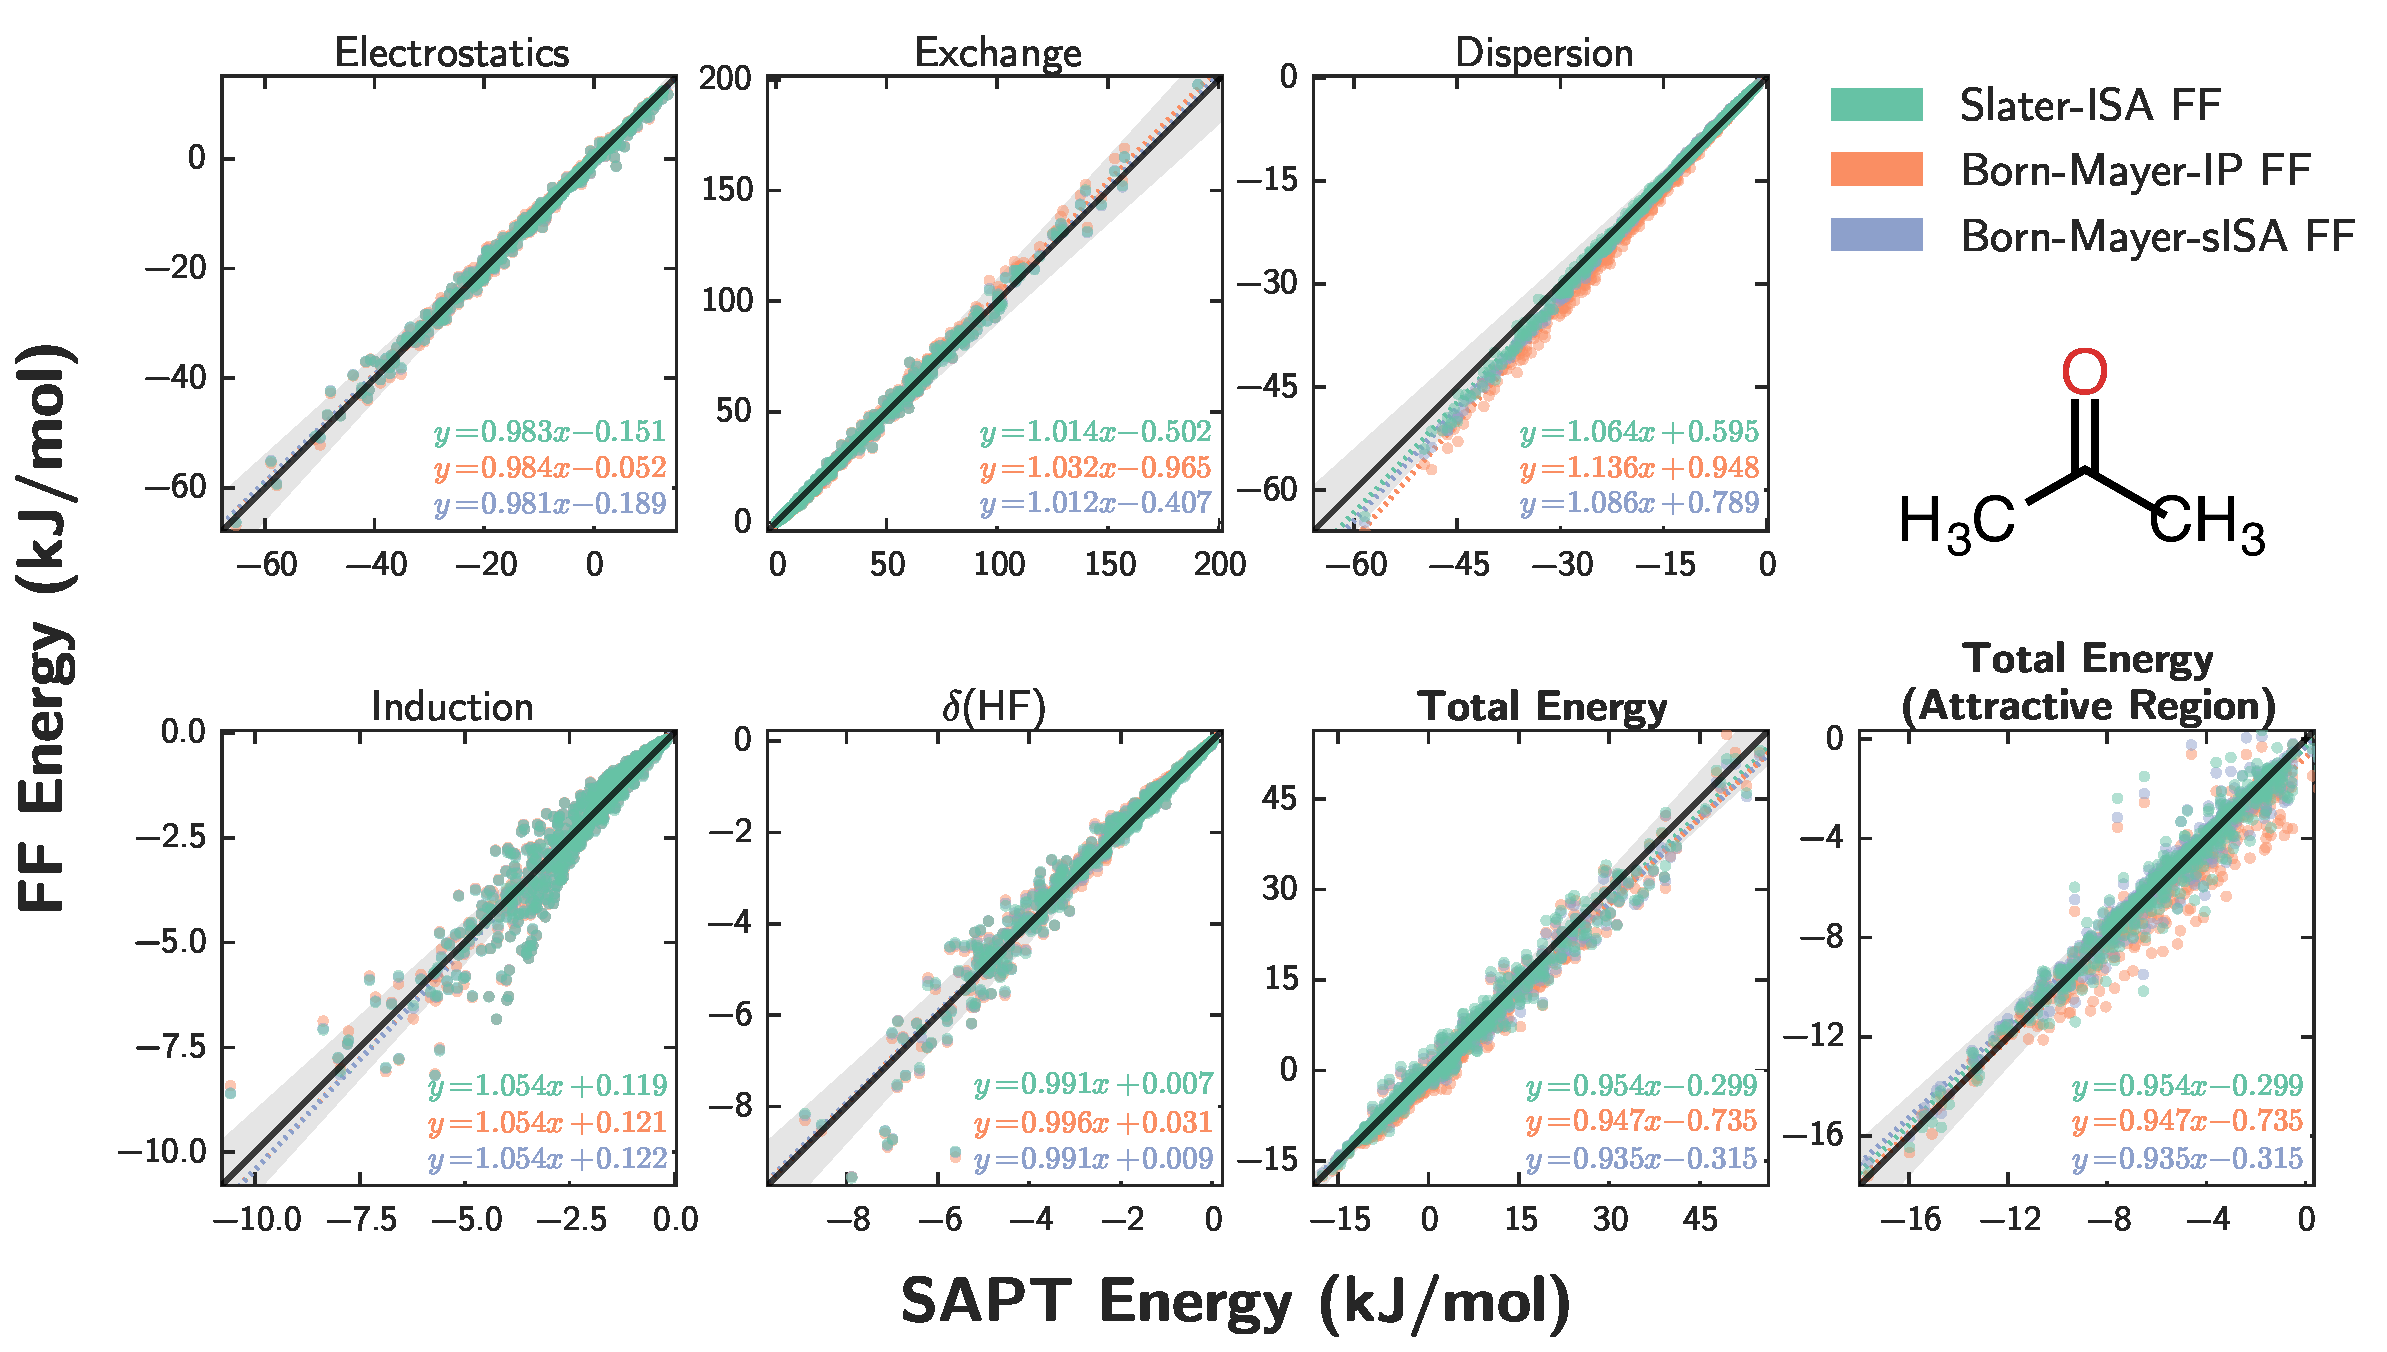
\includegraphics[width=0.9\textwidth]{isotropic/si/acetone_acetone_scatter.pdf}
    \end{subfigure}
    \begin{subfigure}{\textwidth}
        \caption{Ar Dimer}
        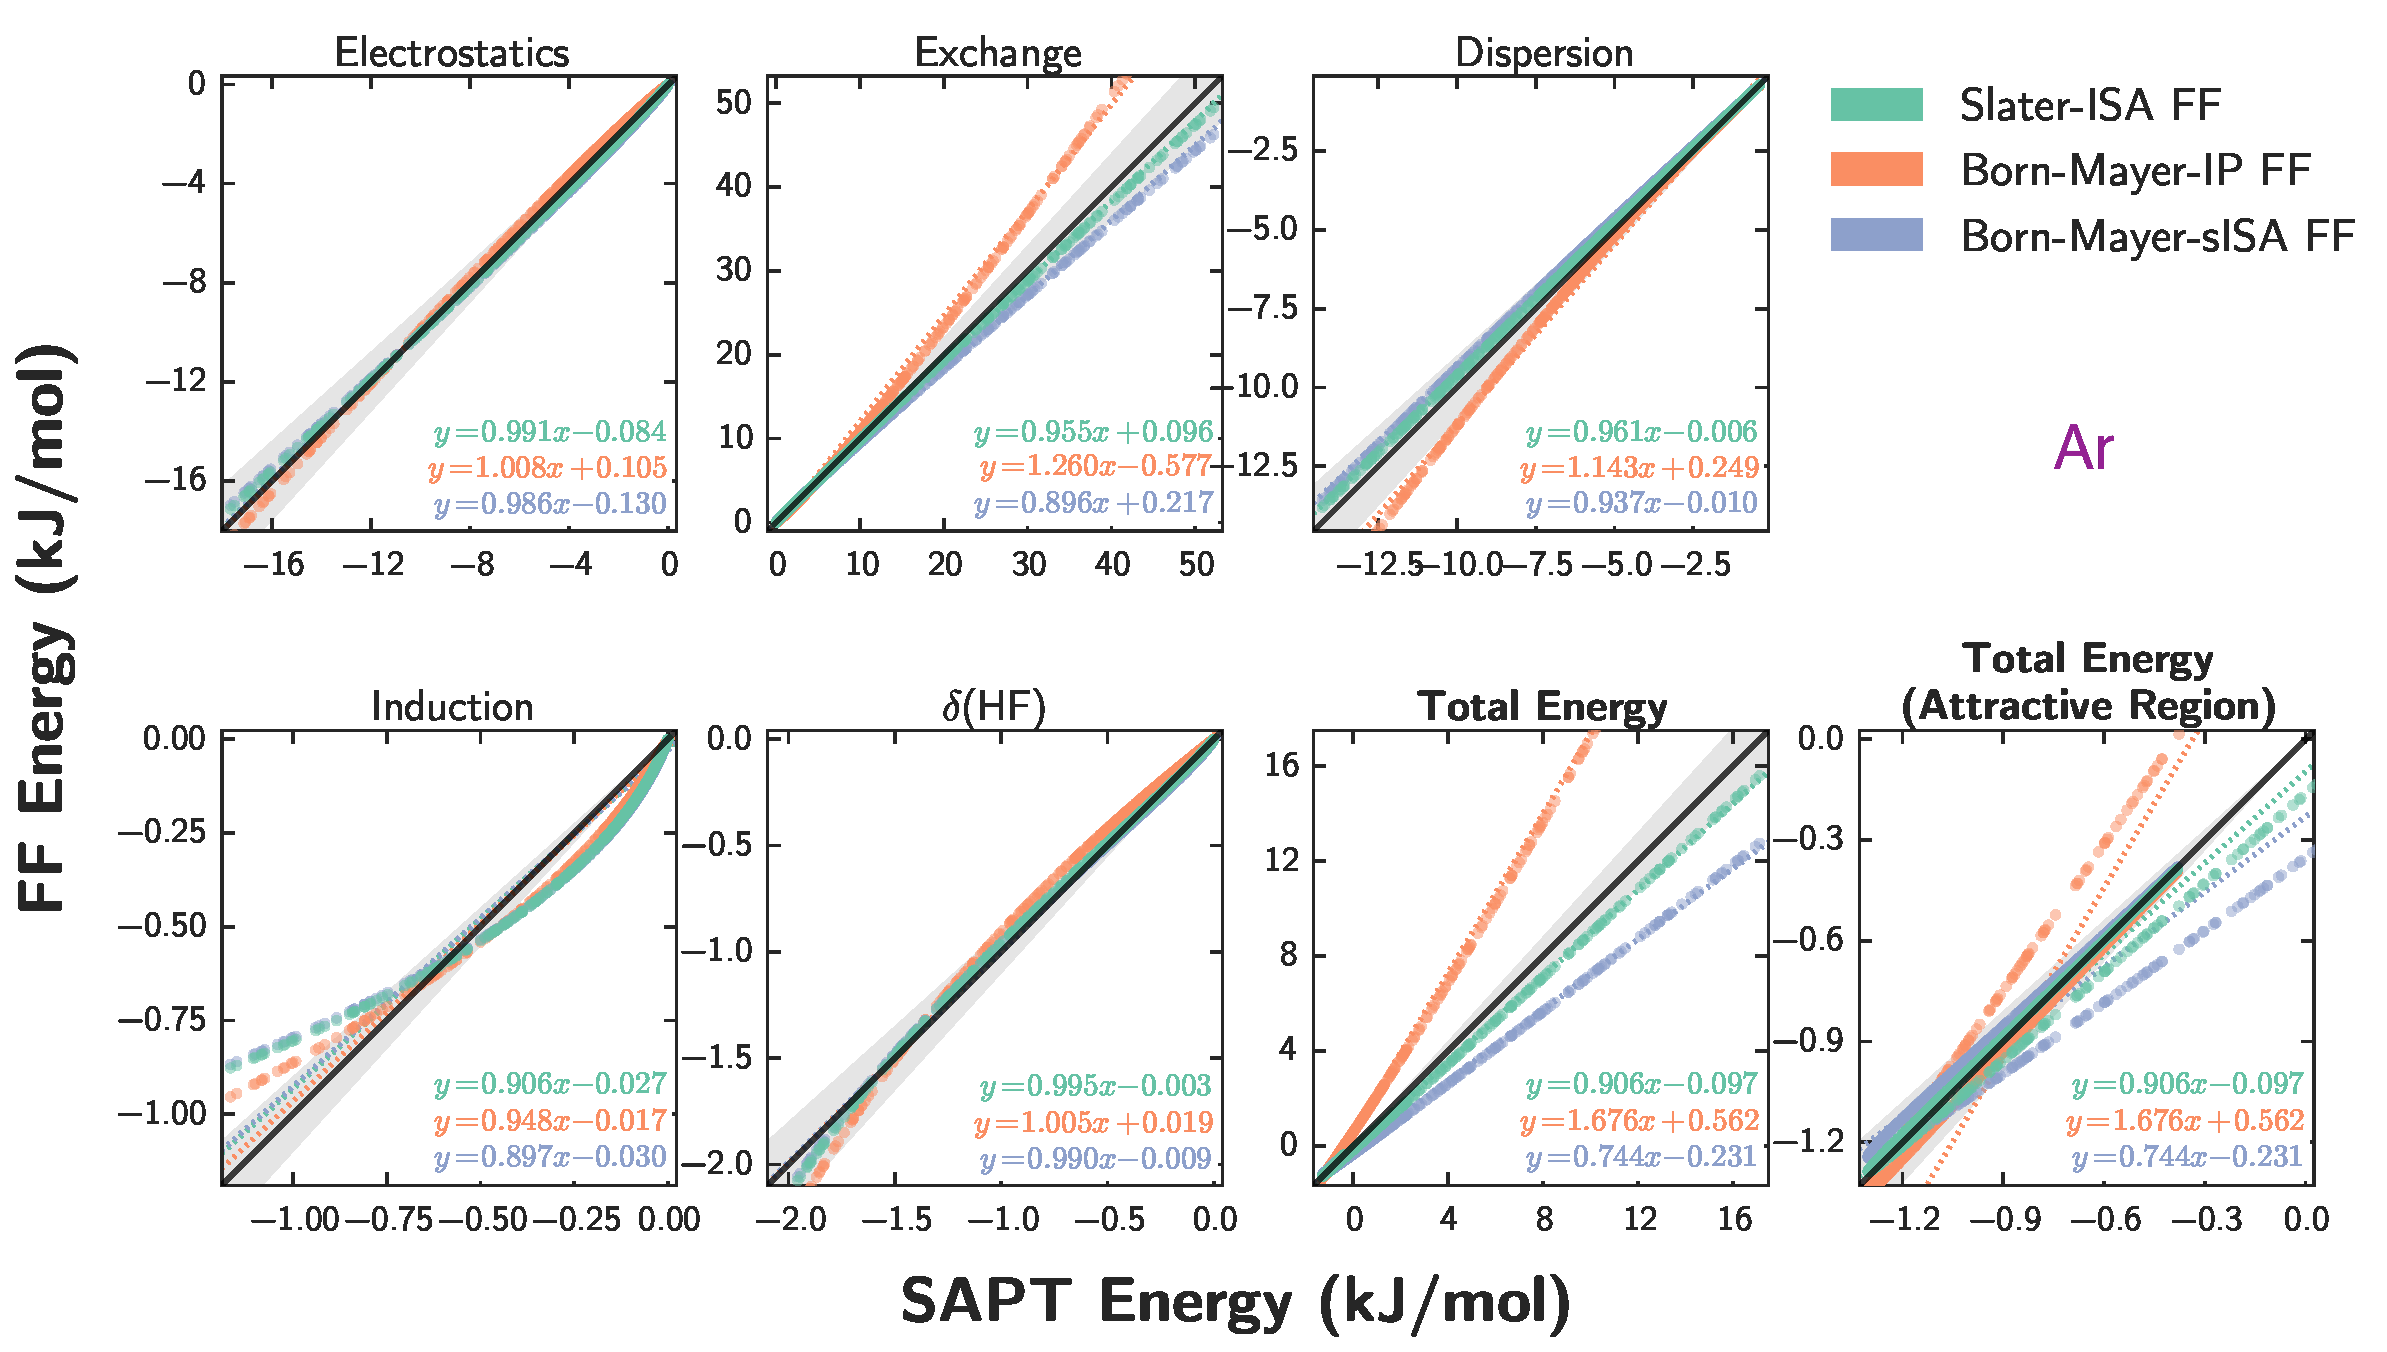
\includegraphics[width=0.9\textwidth]{isotropic/si/ar_ar_scatter.pdf}
    \end{subfigure}
    \end{figure}
    \begin{figure}
    \ContinuedFloat
    \begin{subfigure}{\textwidth}
        \caption{Chloromethane Dimer}
        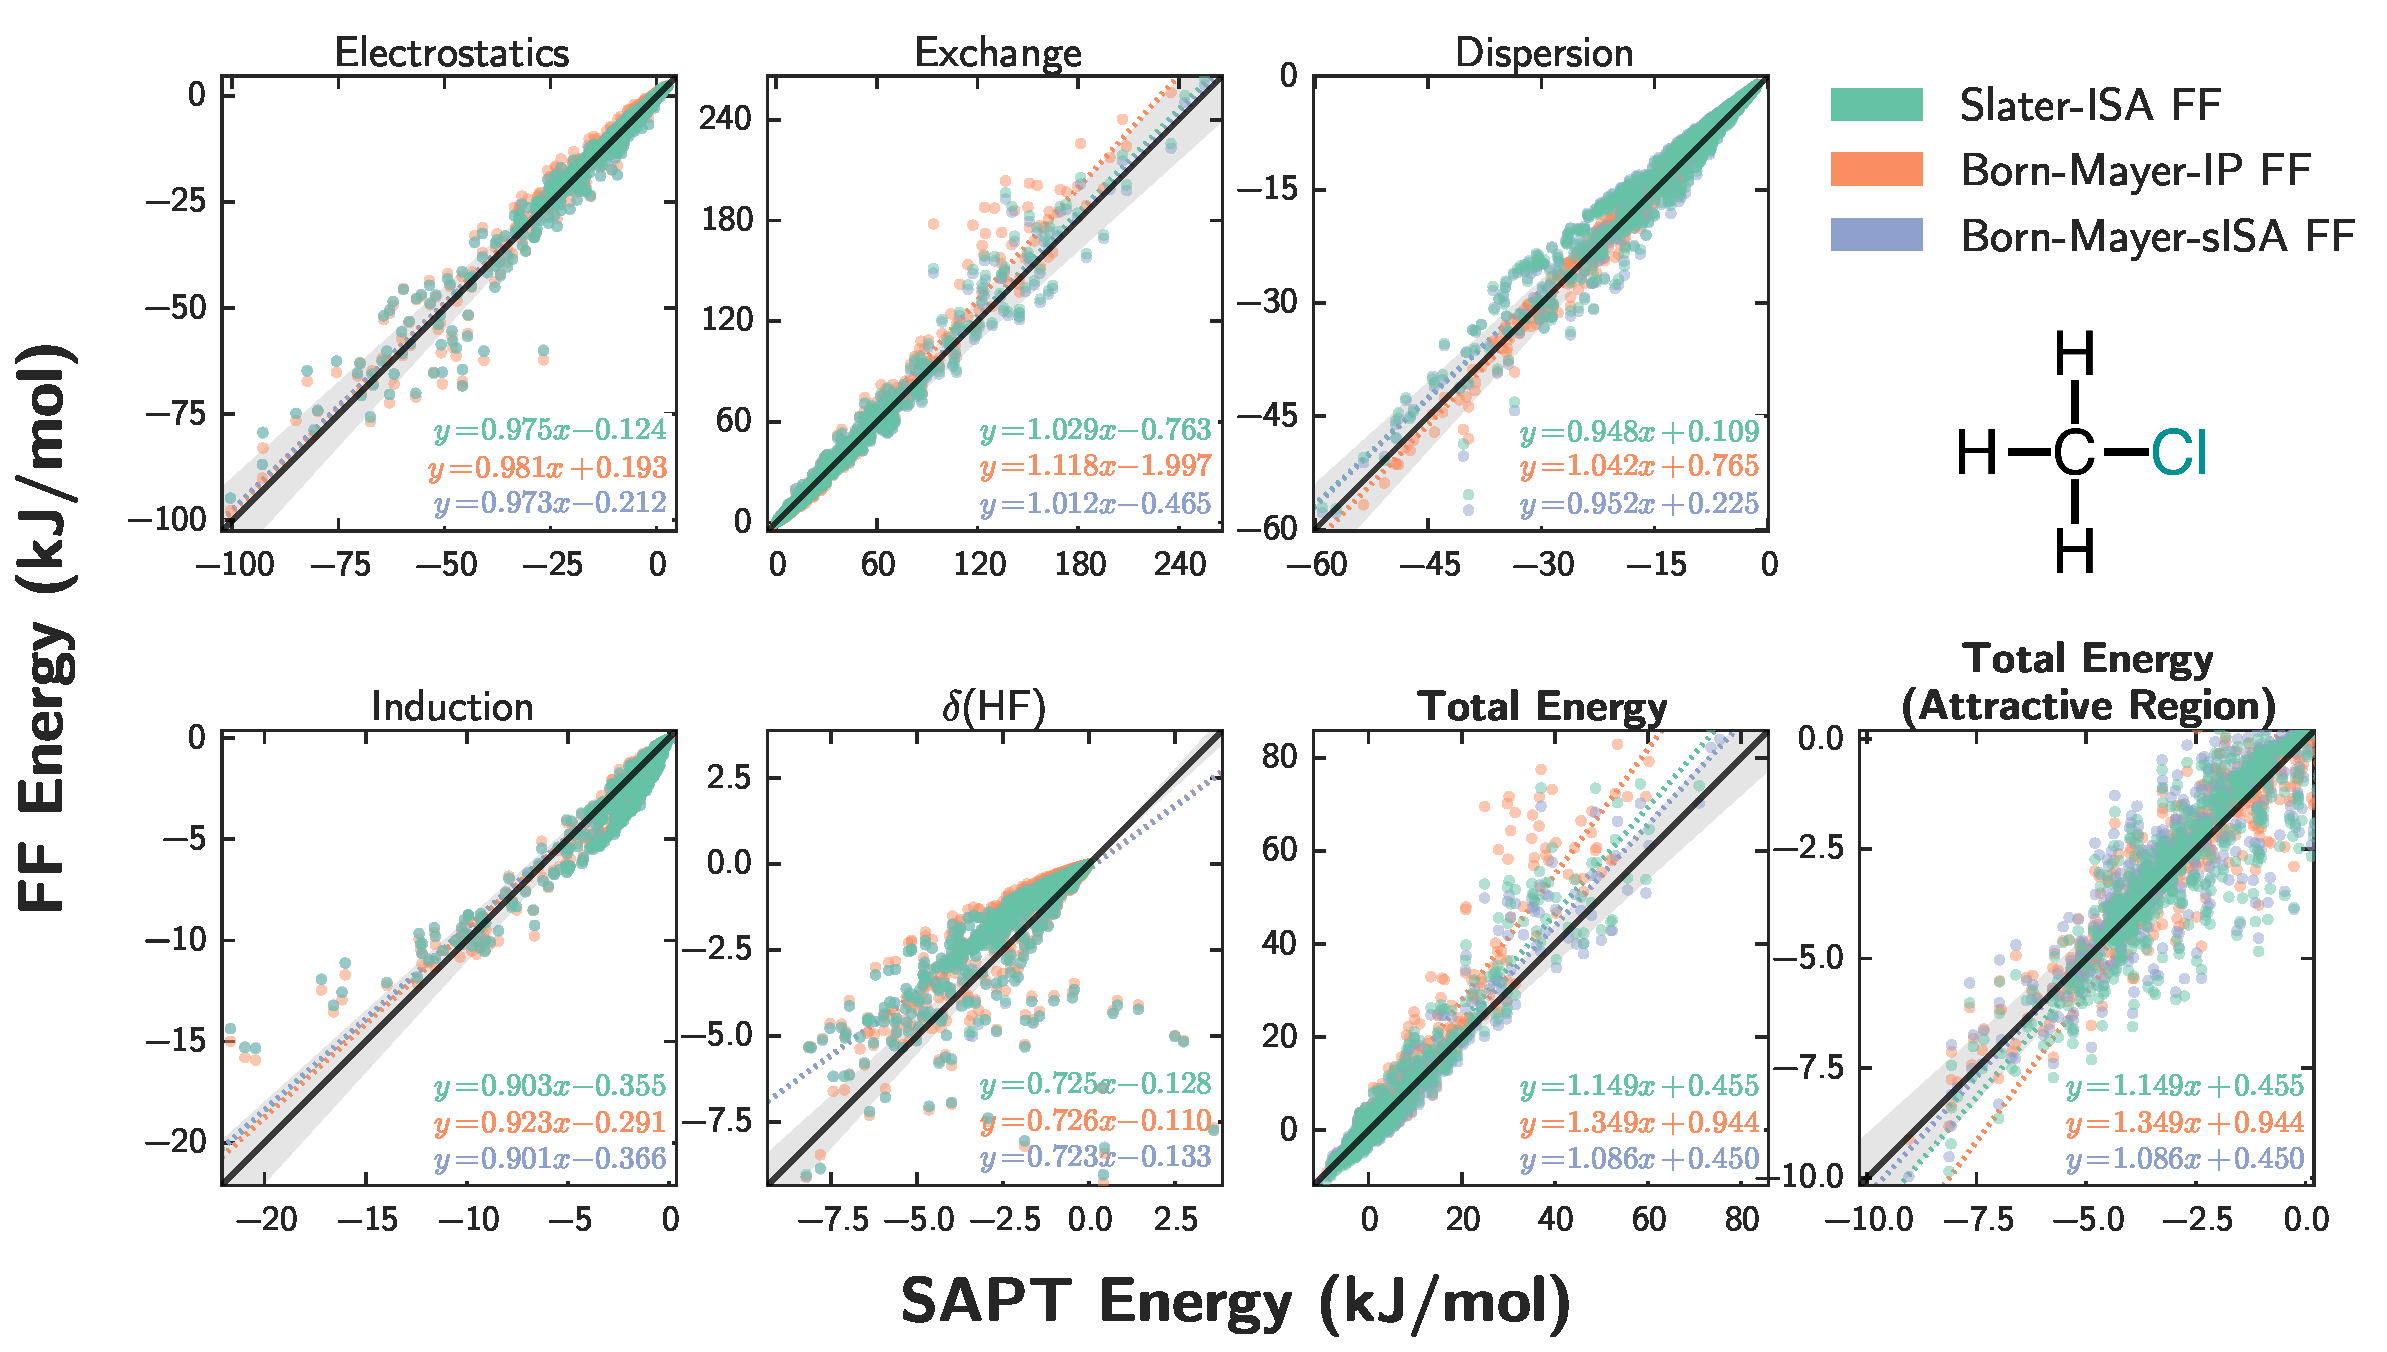
\includegraphics[width=0.9\textwidth]{isotropic/si/chloromethane_chloromethane_scatter.pdf}
    \end{subfigure}
    \begin{subfigure}{\textwidth}
        \caption{\co Dimer}
        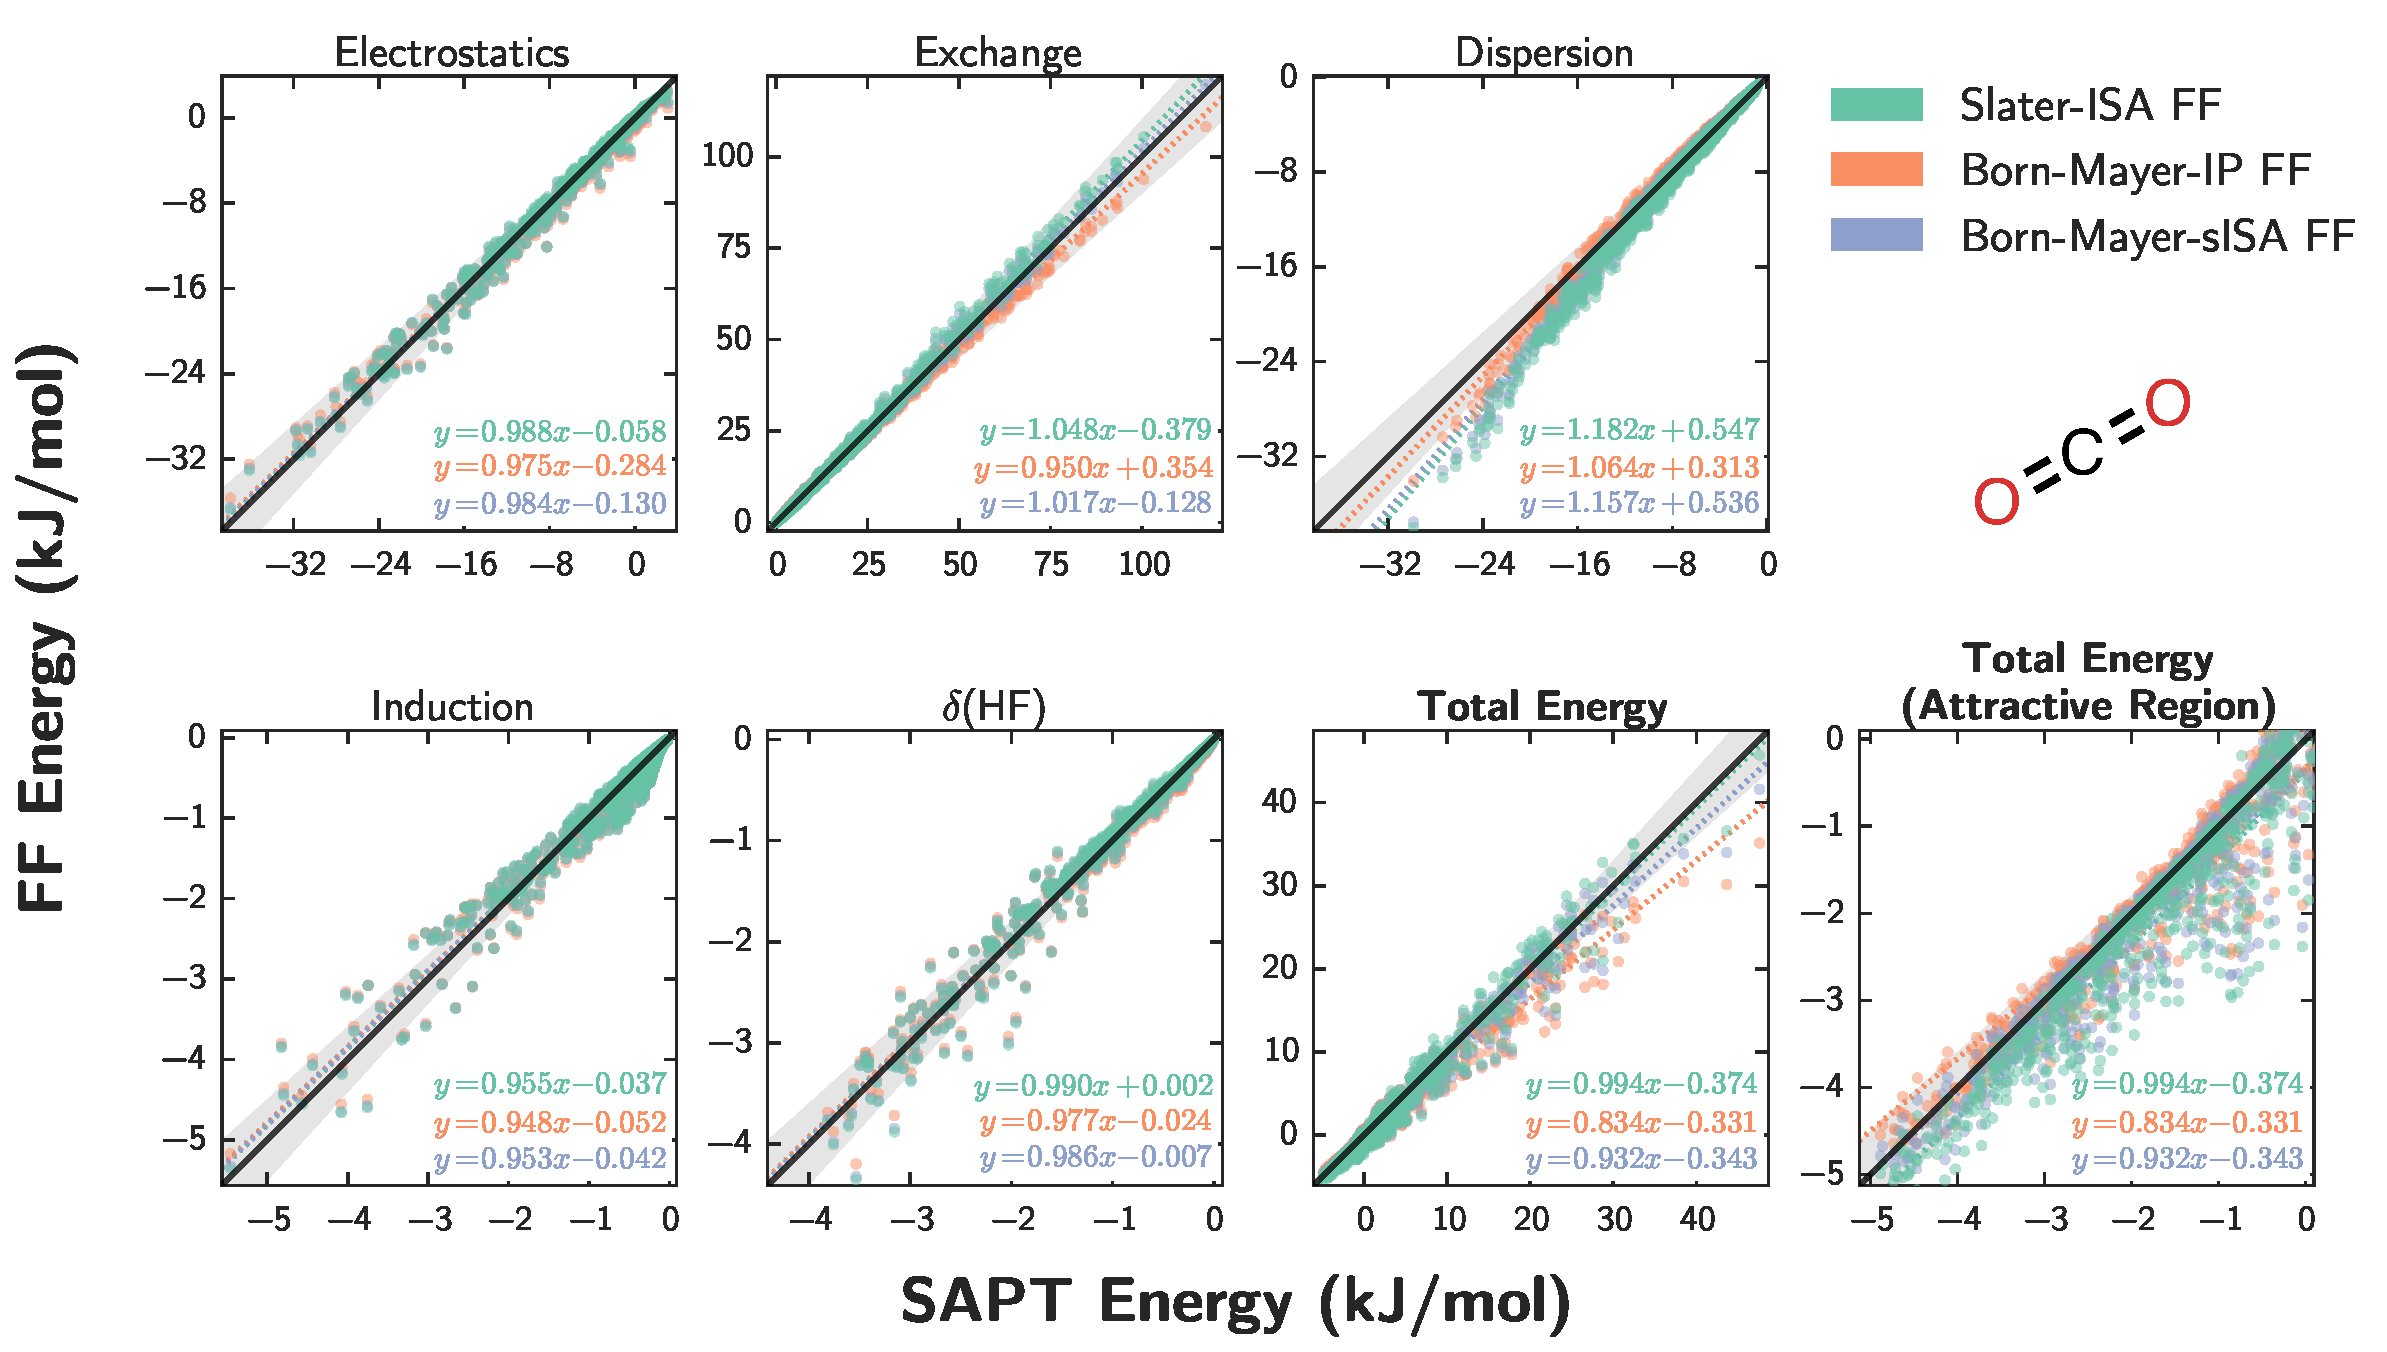
\includegraphics[width=0.9\textwidth]{isotropic/si/co2_co2_scatter.pdf}
    \end{subfigure}
    \end{figure}
    \begin{figure}
    \ContinuedFloat
    \begin{subfigure}{\textwidth}
        \caption{Dimethyl Ether Dimer}
        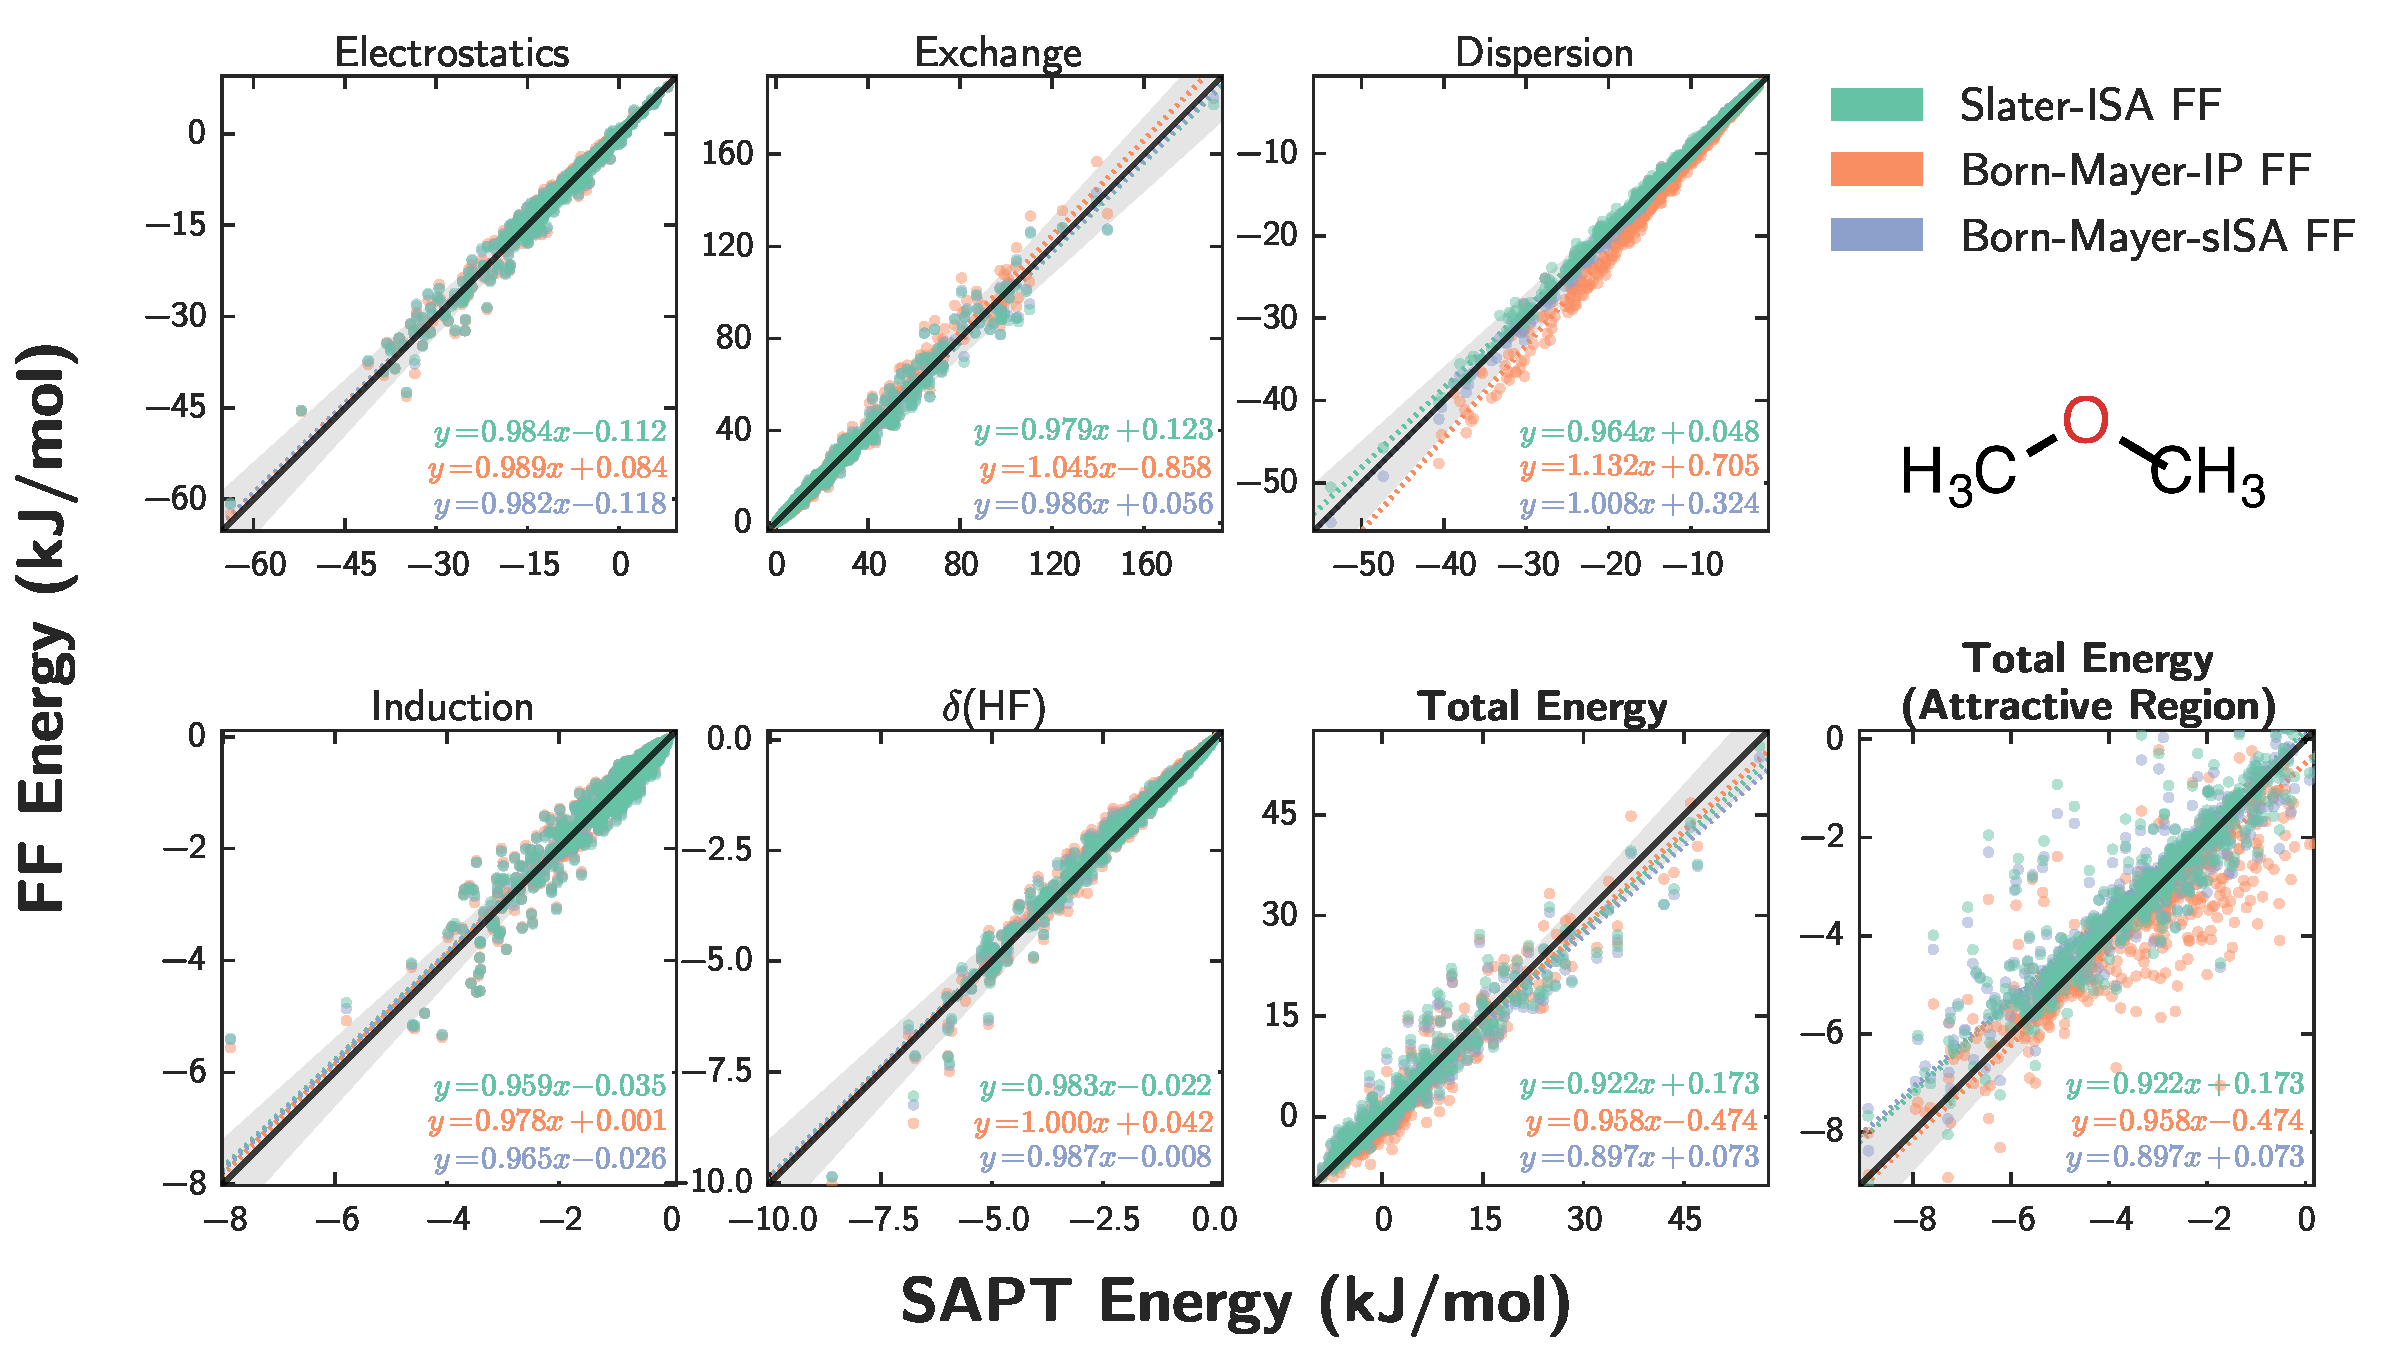
\includegraphics[width=0.9\textwidth]{isotropic/si/dimethyl_ether_dimethyl_ether_scatter.pdf}
    \end{subfigure}
    \begin{subfigure}{\textwidth}
        \caption{Ethane Dimer}
        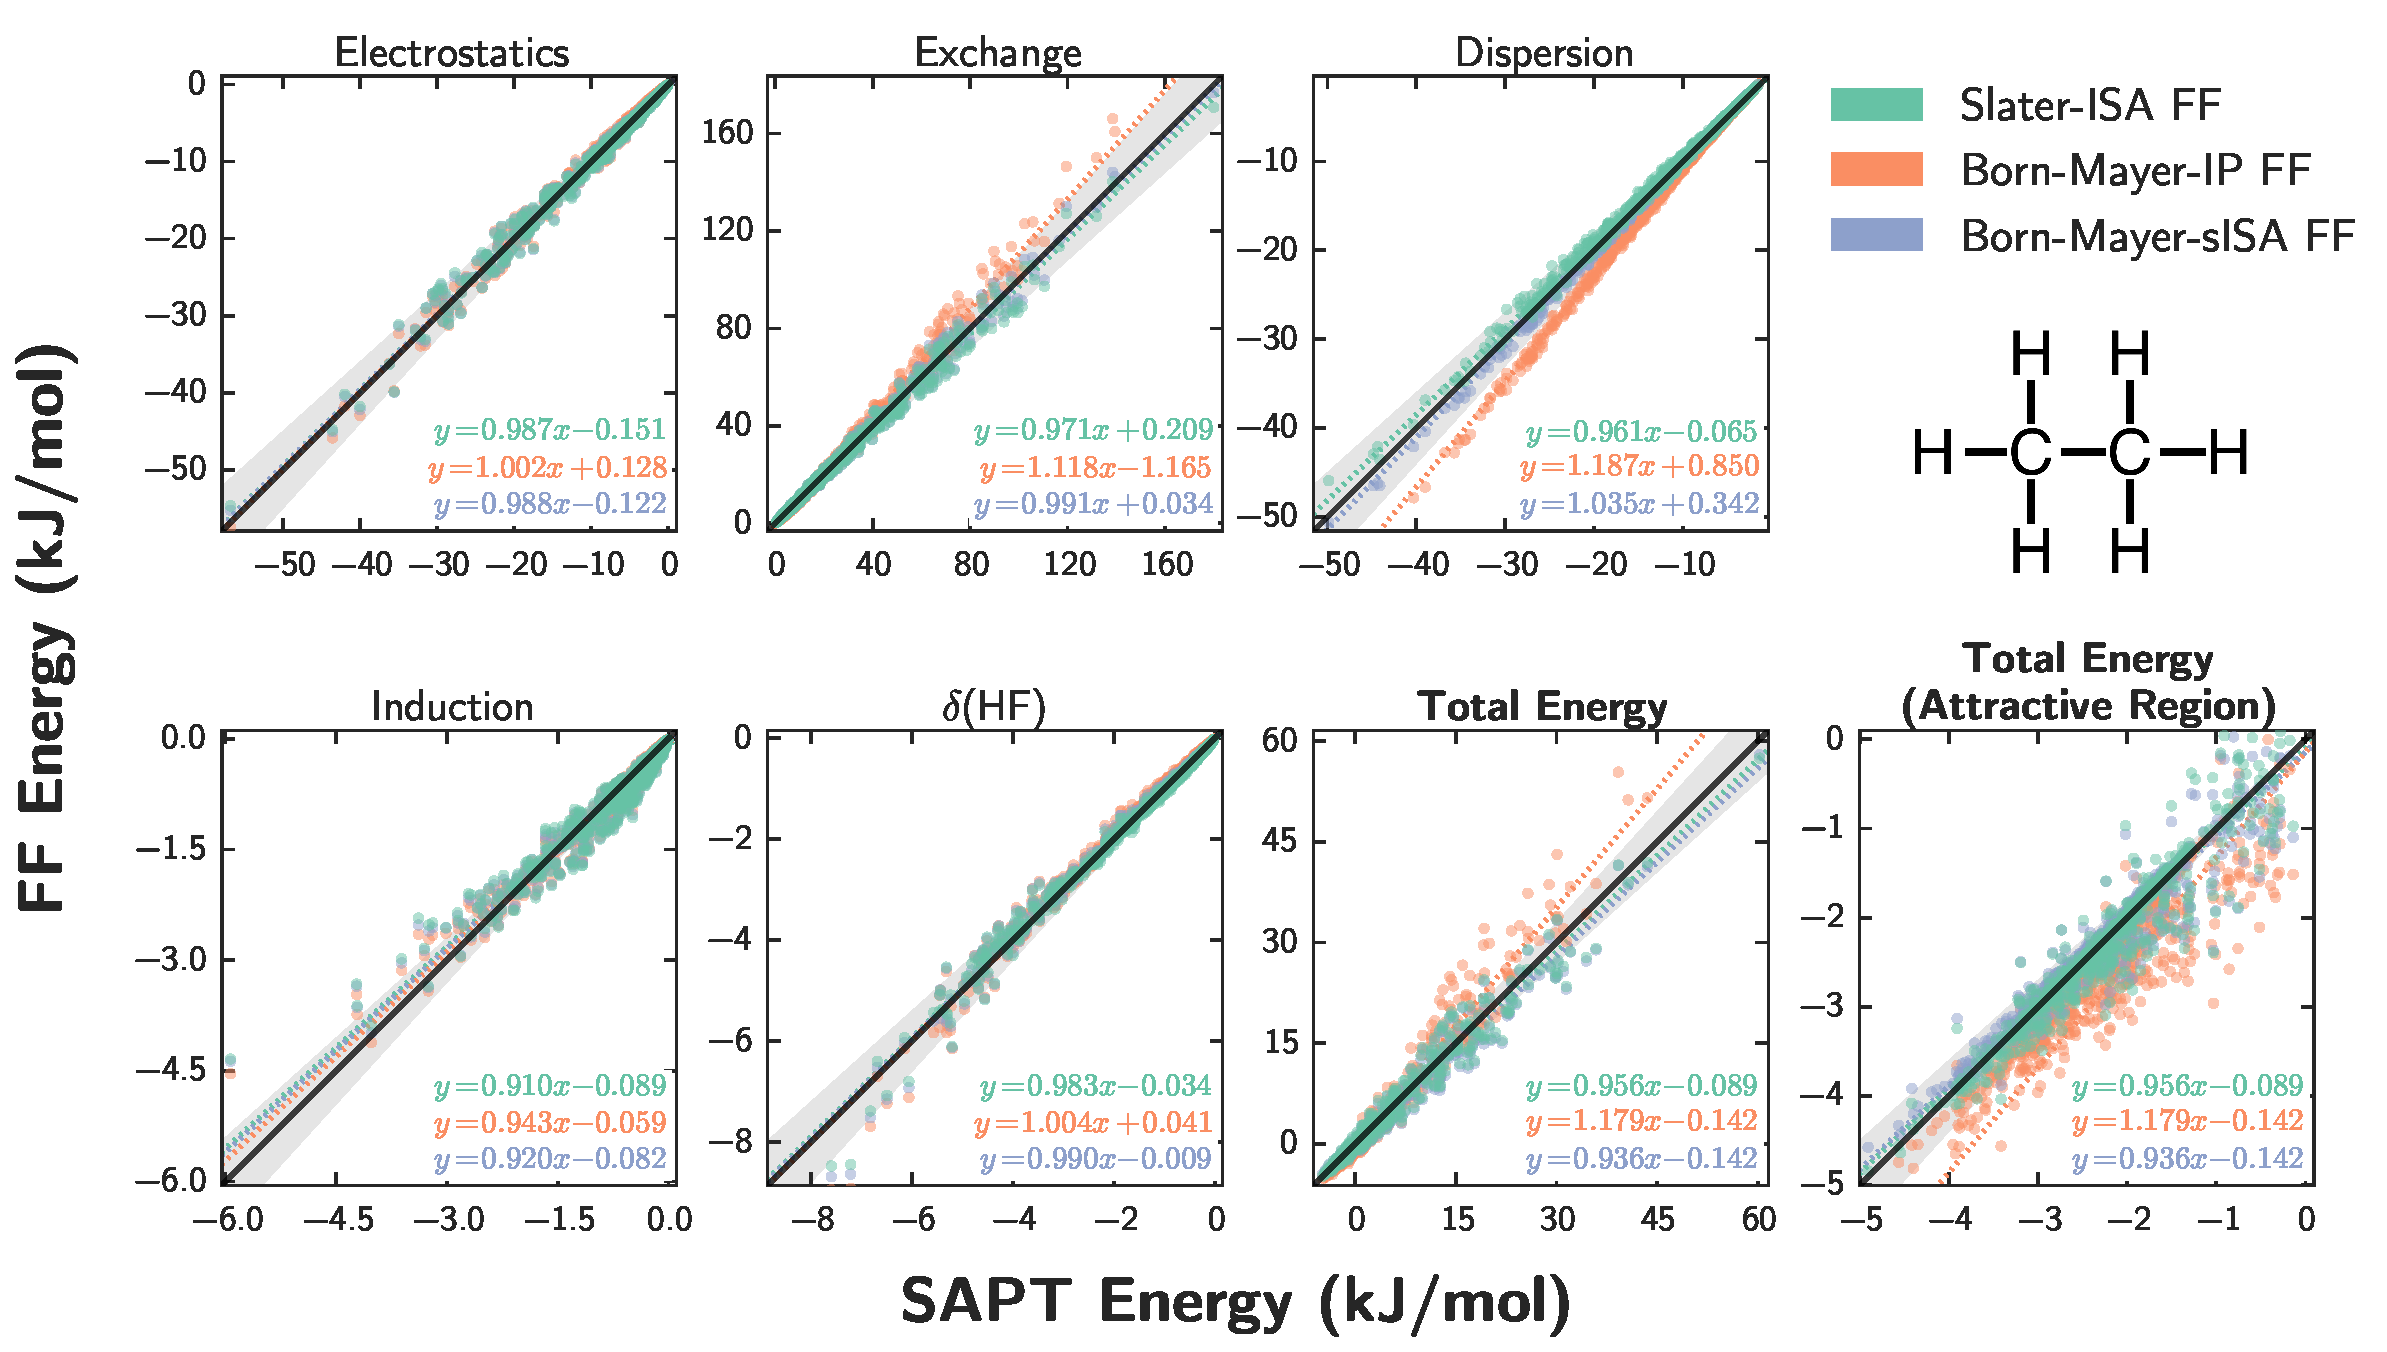
\includegraphics[width=0.9\textwidth]{isotropic/si/ethane_ethane_scatter.pdf}
    \end{subfigure}
    \end{figure}
    \begin{figure}
    \ContinuedFloat
    \begin{subfigure}{\textwidth}
        \caption{Ethanol Dimer}
        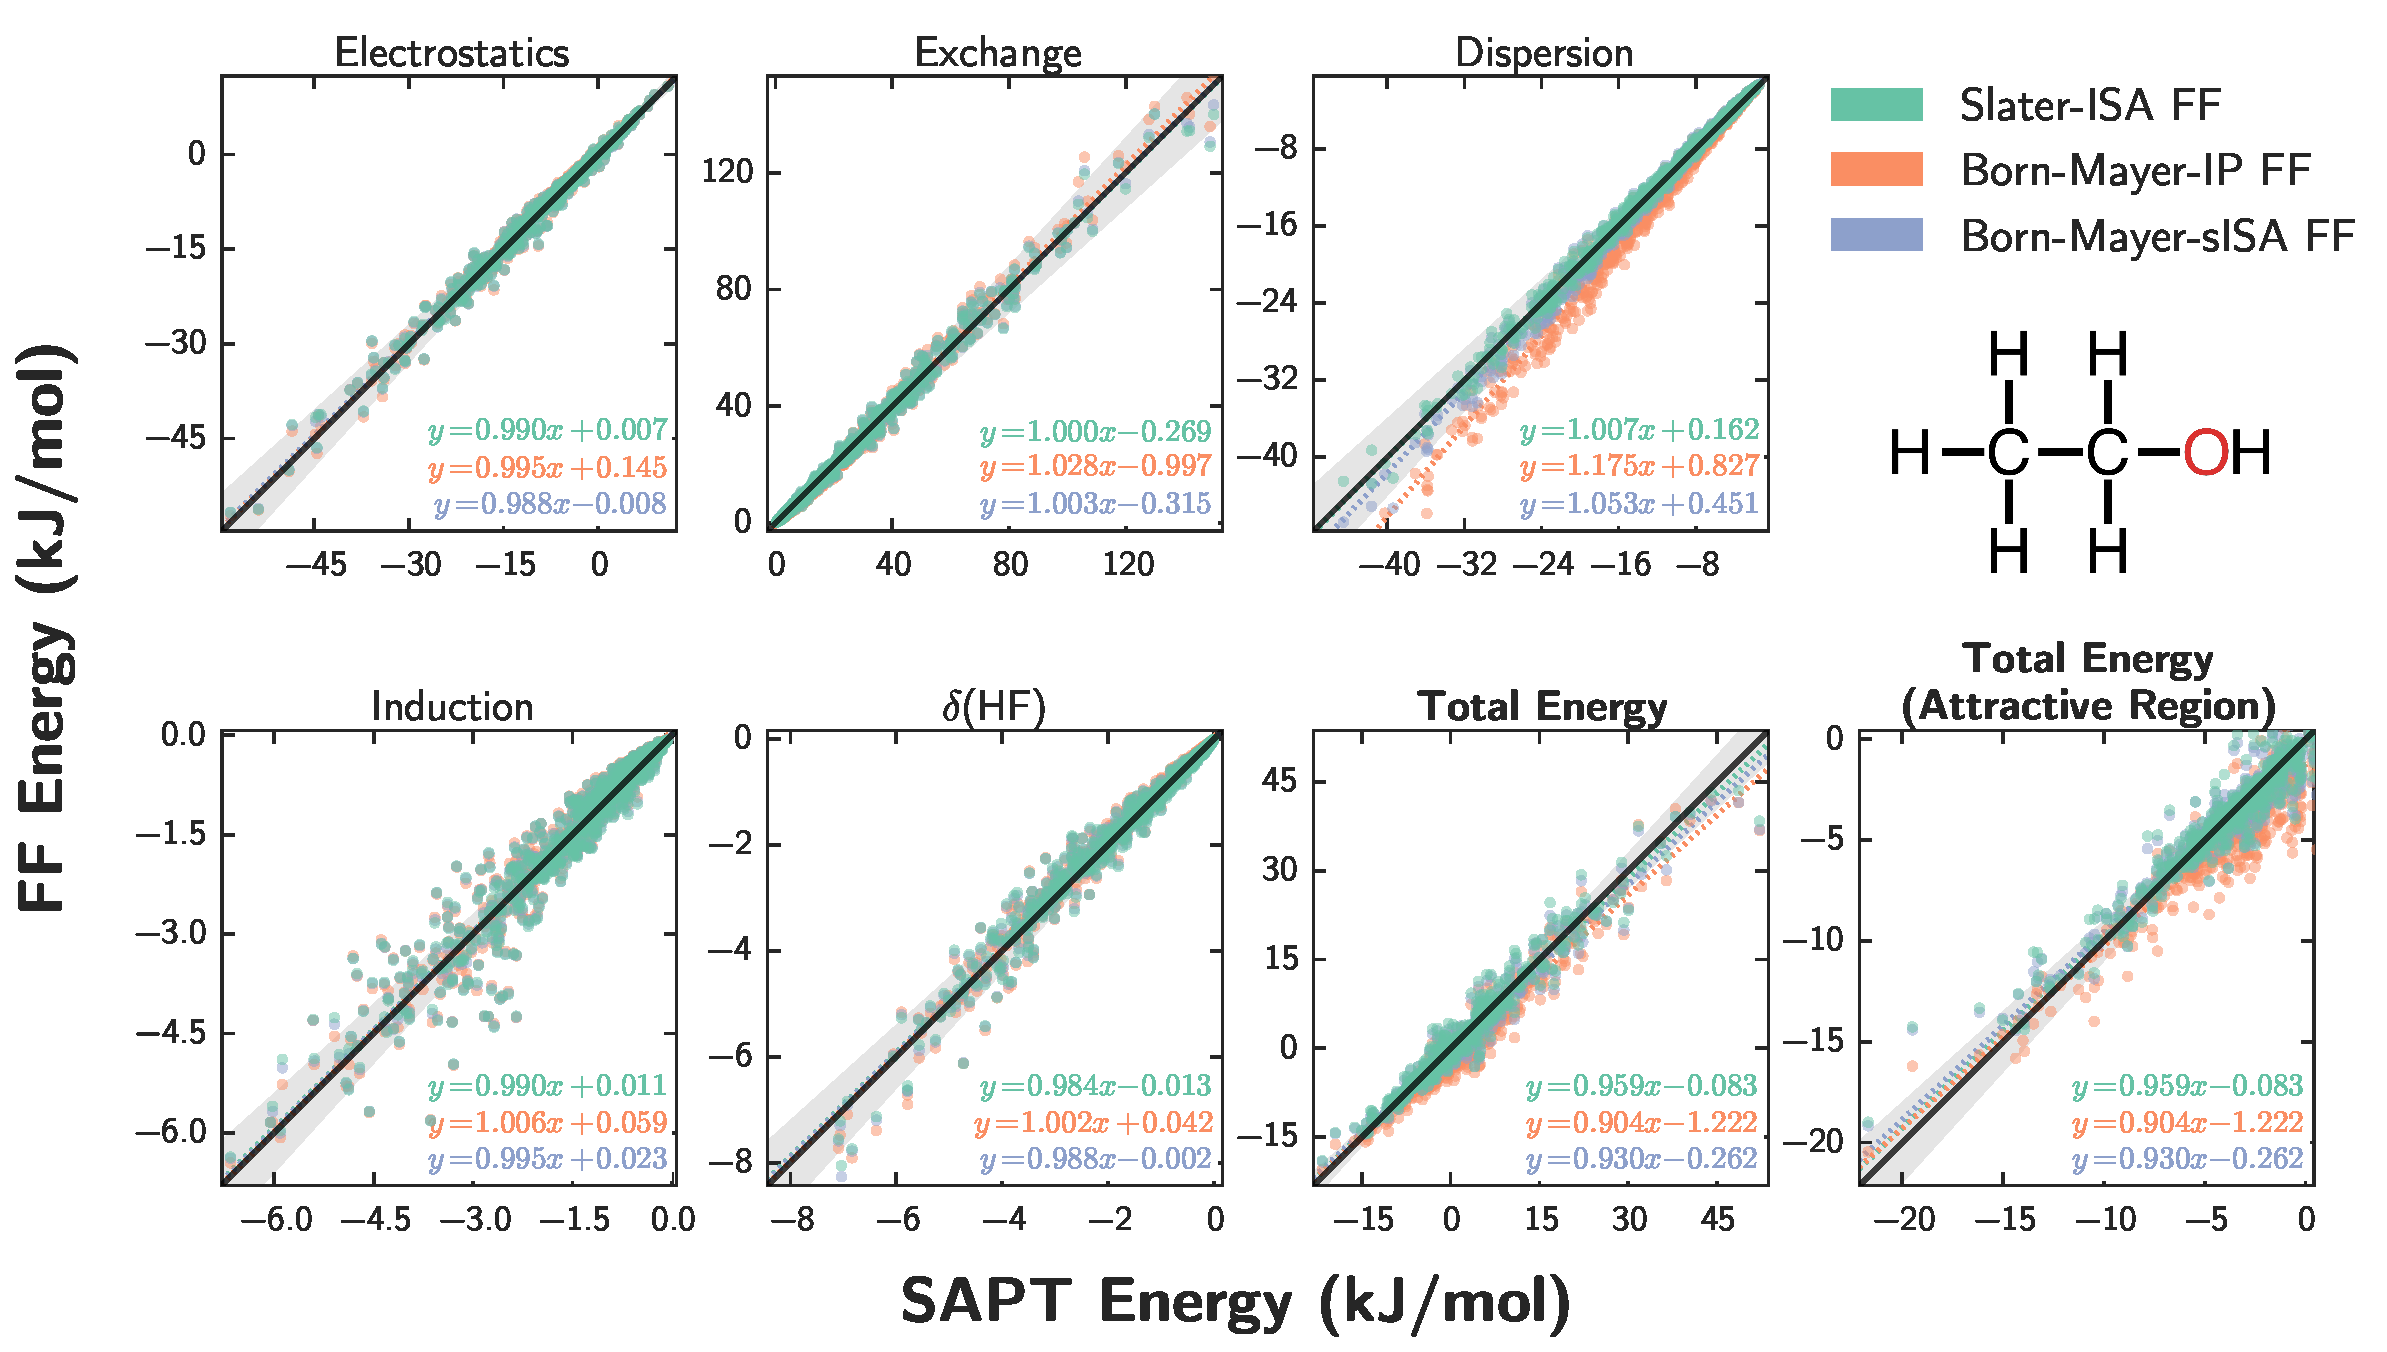
\includegraphics[width=0.9\textwidth]{isotropic/si/ethanol_ethanol_scatter.pdf}
    \end{subfigure}
    \begin{subfigure}{\textwidth}
        \caption{Ethene Dimer}
        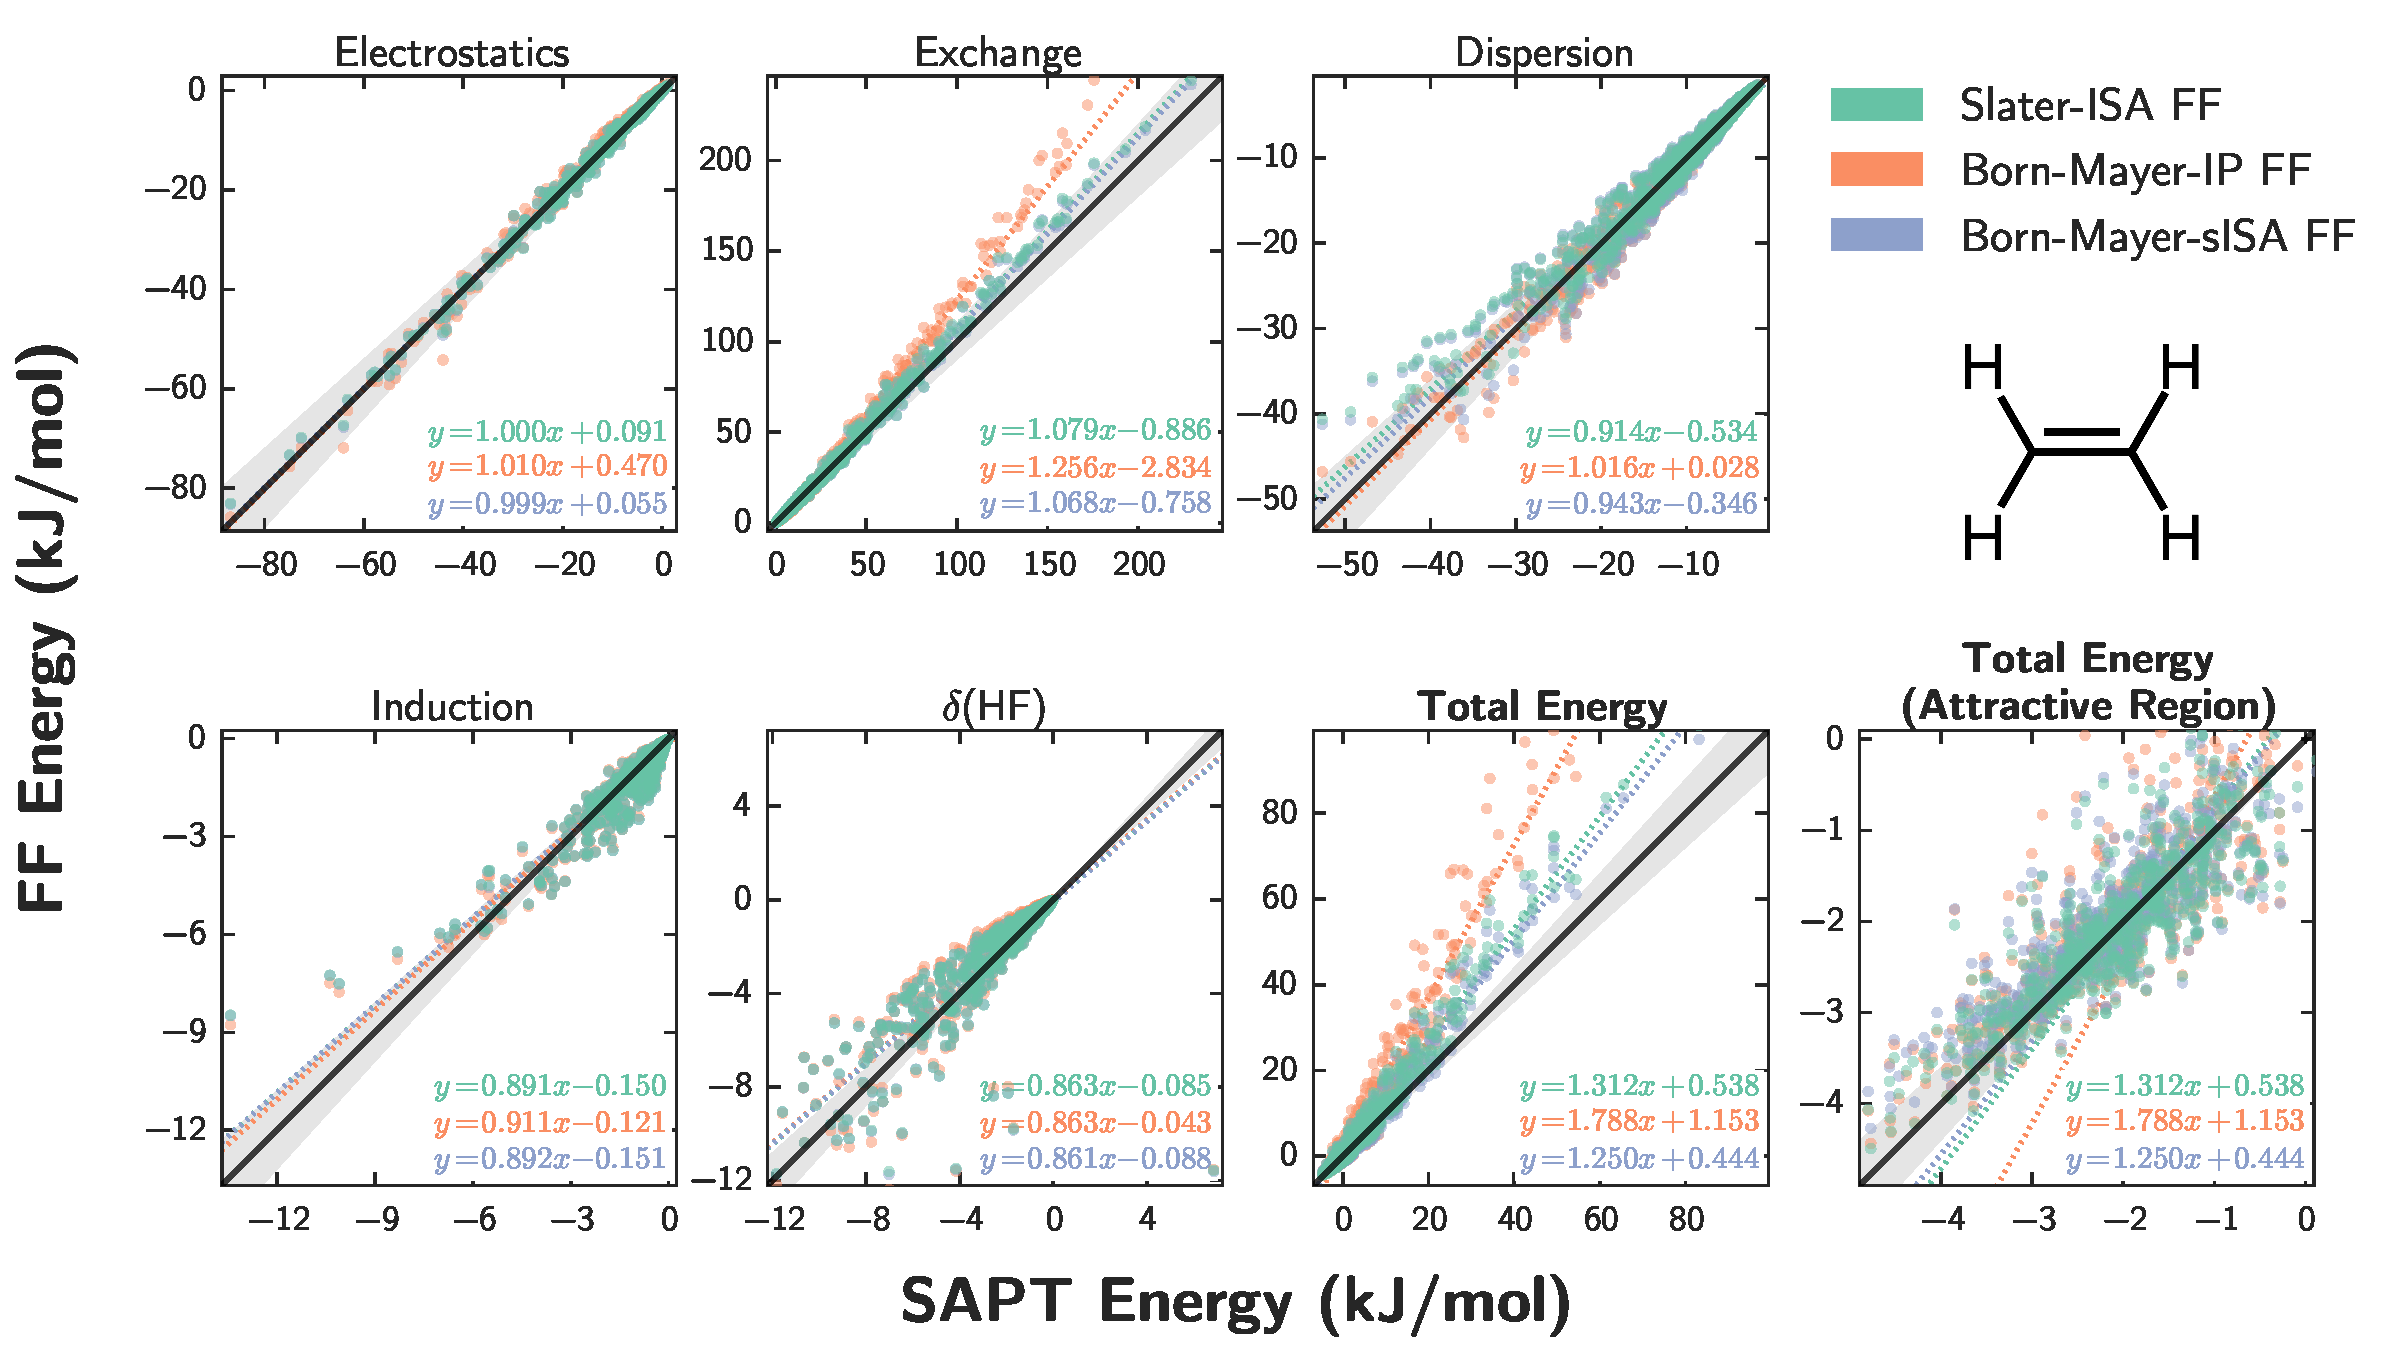
\includegraphics[width=0.9\textwidth]{isotropic/si/ethene_ethene_scatter.pdf}
    \end{subfigure}
    \end{figure}
    \begin{figure}
    \ContinuedFloat
    \begin{subfigure}{\textwidth}
        \caption{\ho Dimer}
        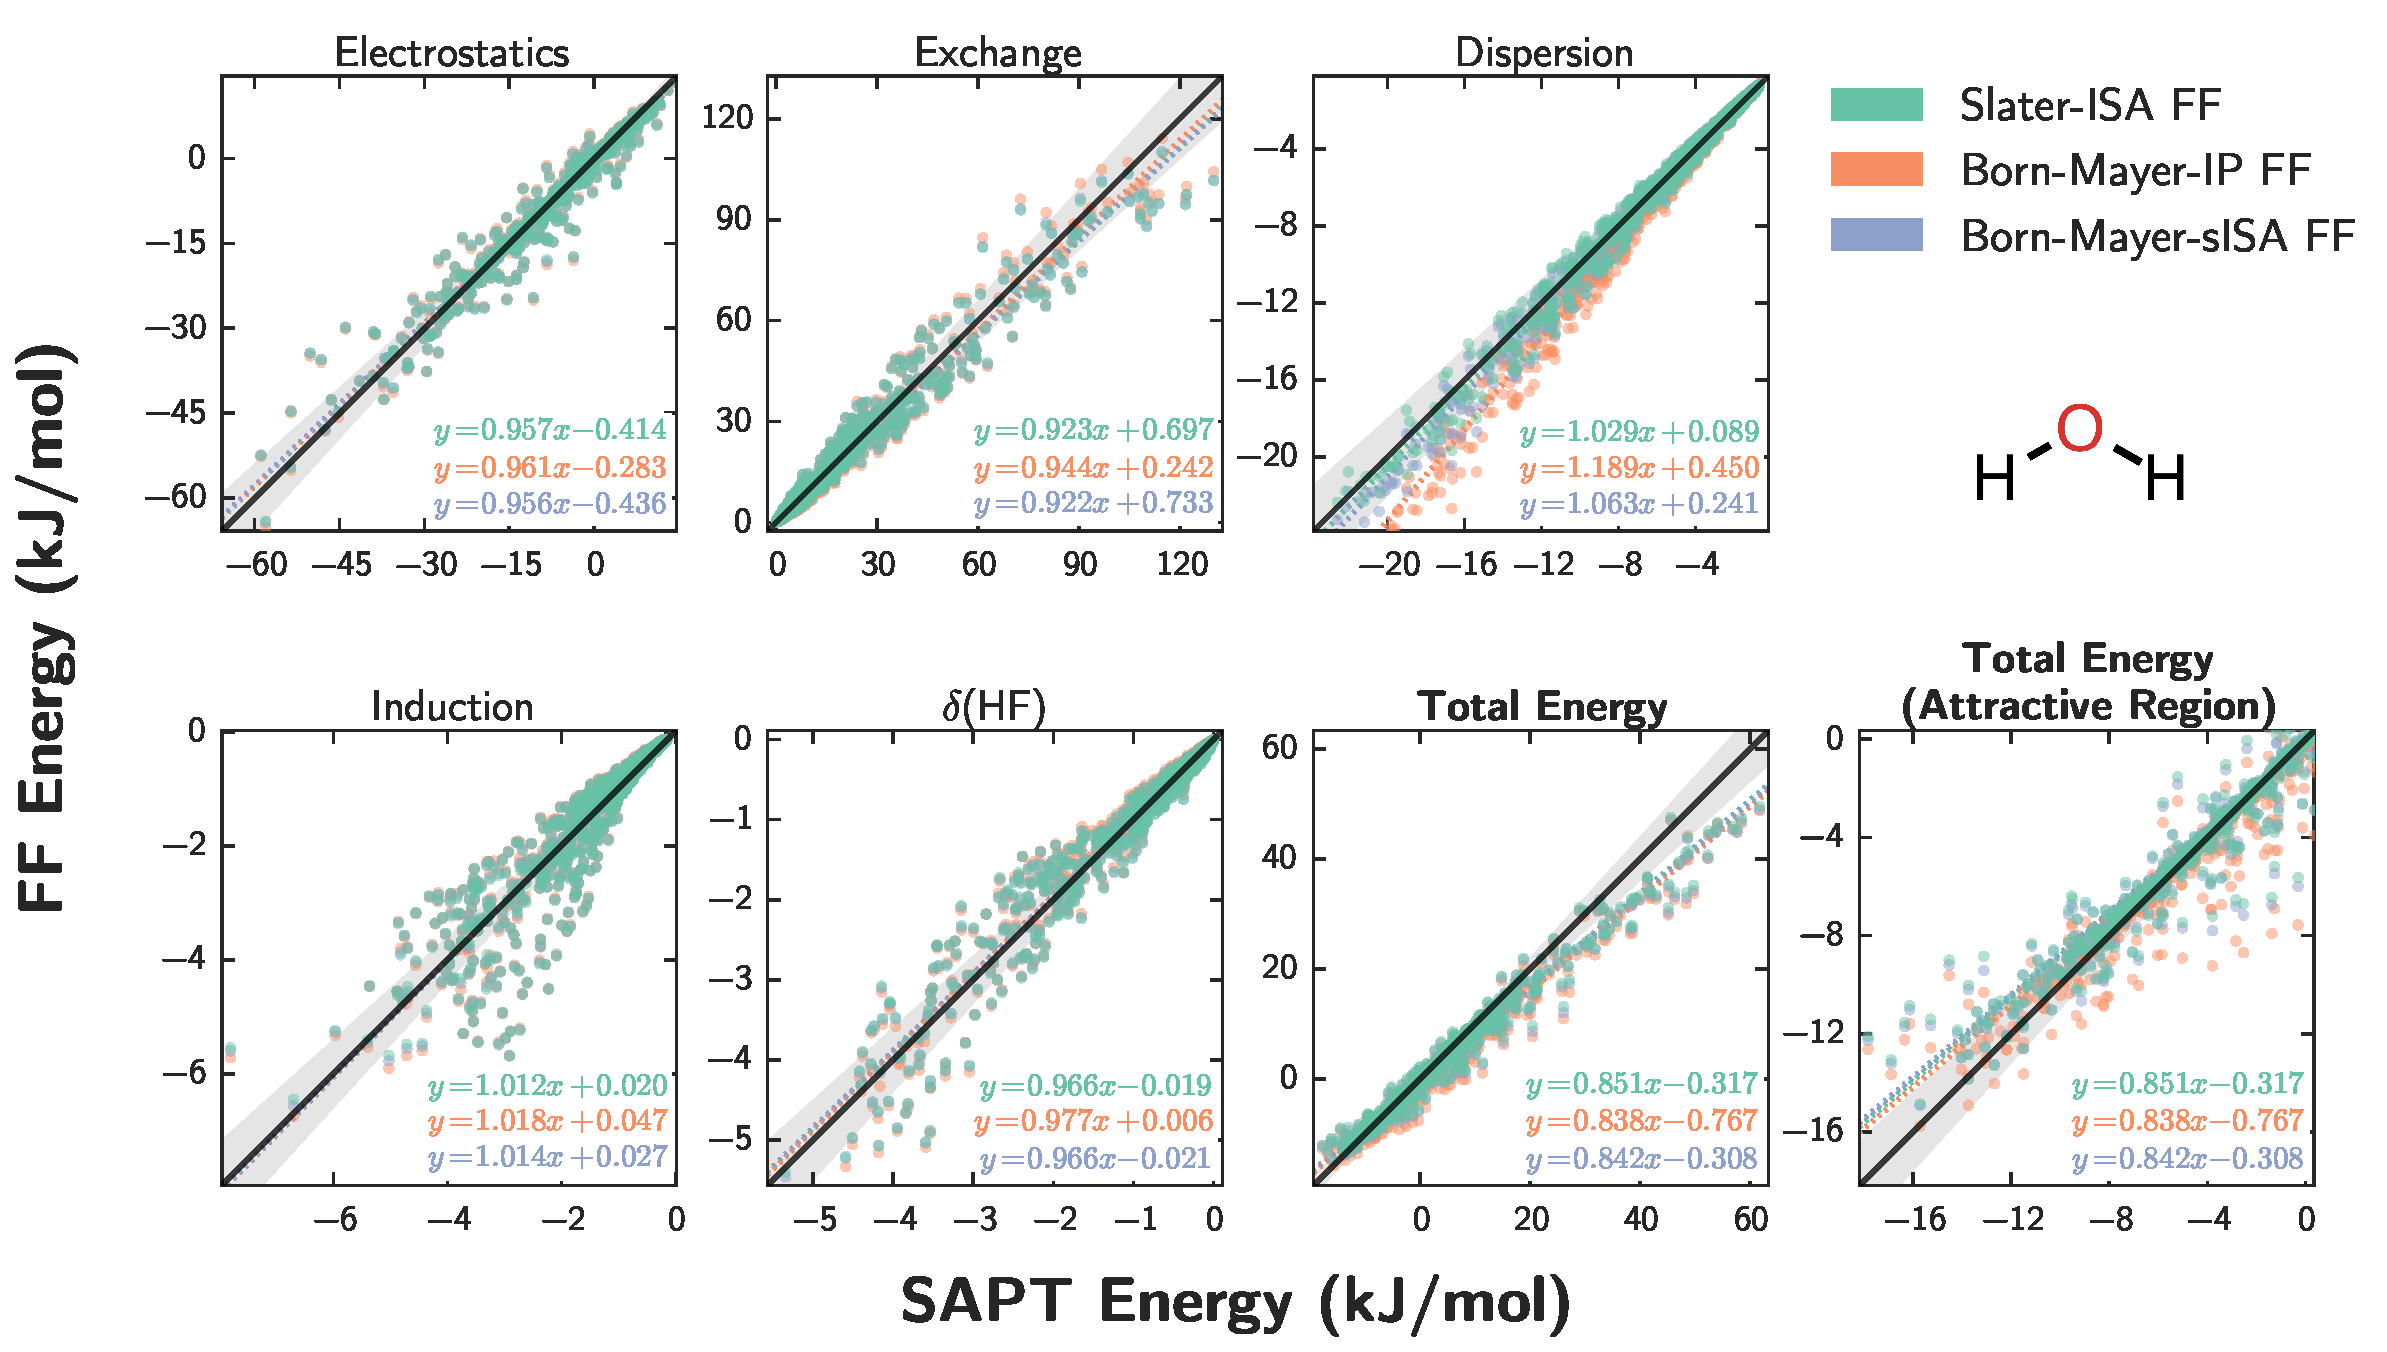
\includegraphics[width=0.9\textwidth]{isotropic/si/h2o_h2o_scatter.pdf}
    \end{subfigure}
    \begin{subfigure}{\textwidth}
        \caption{Methane Dimer}
        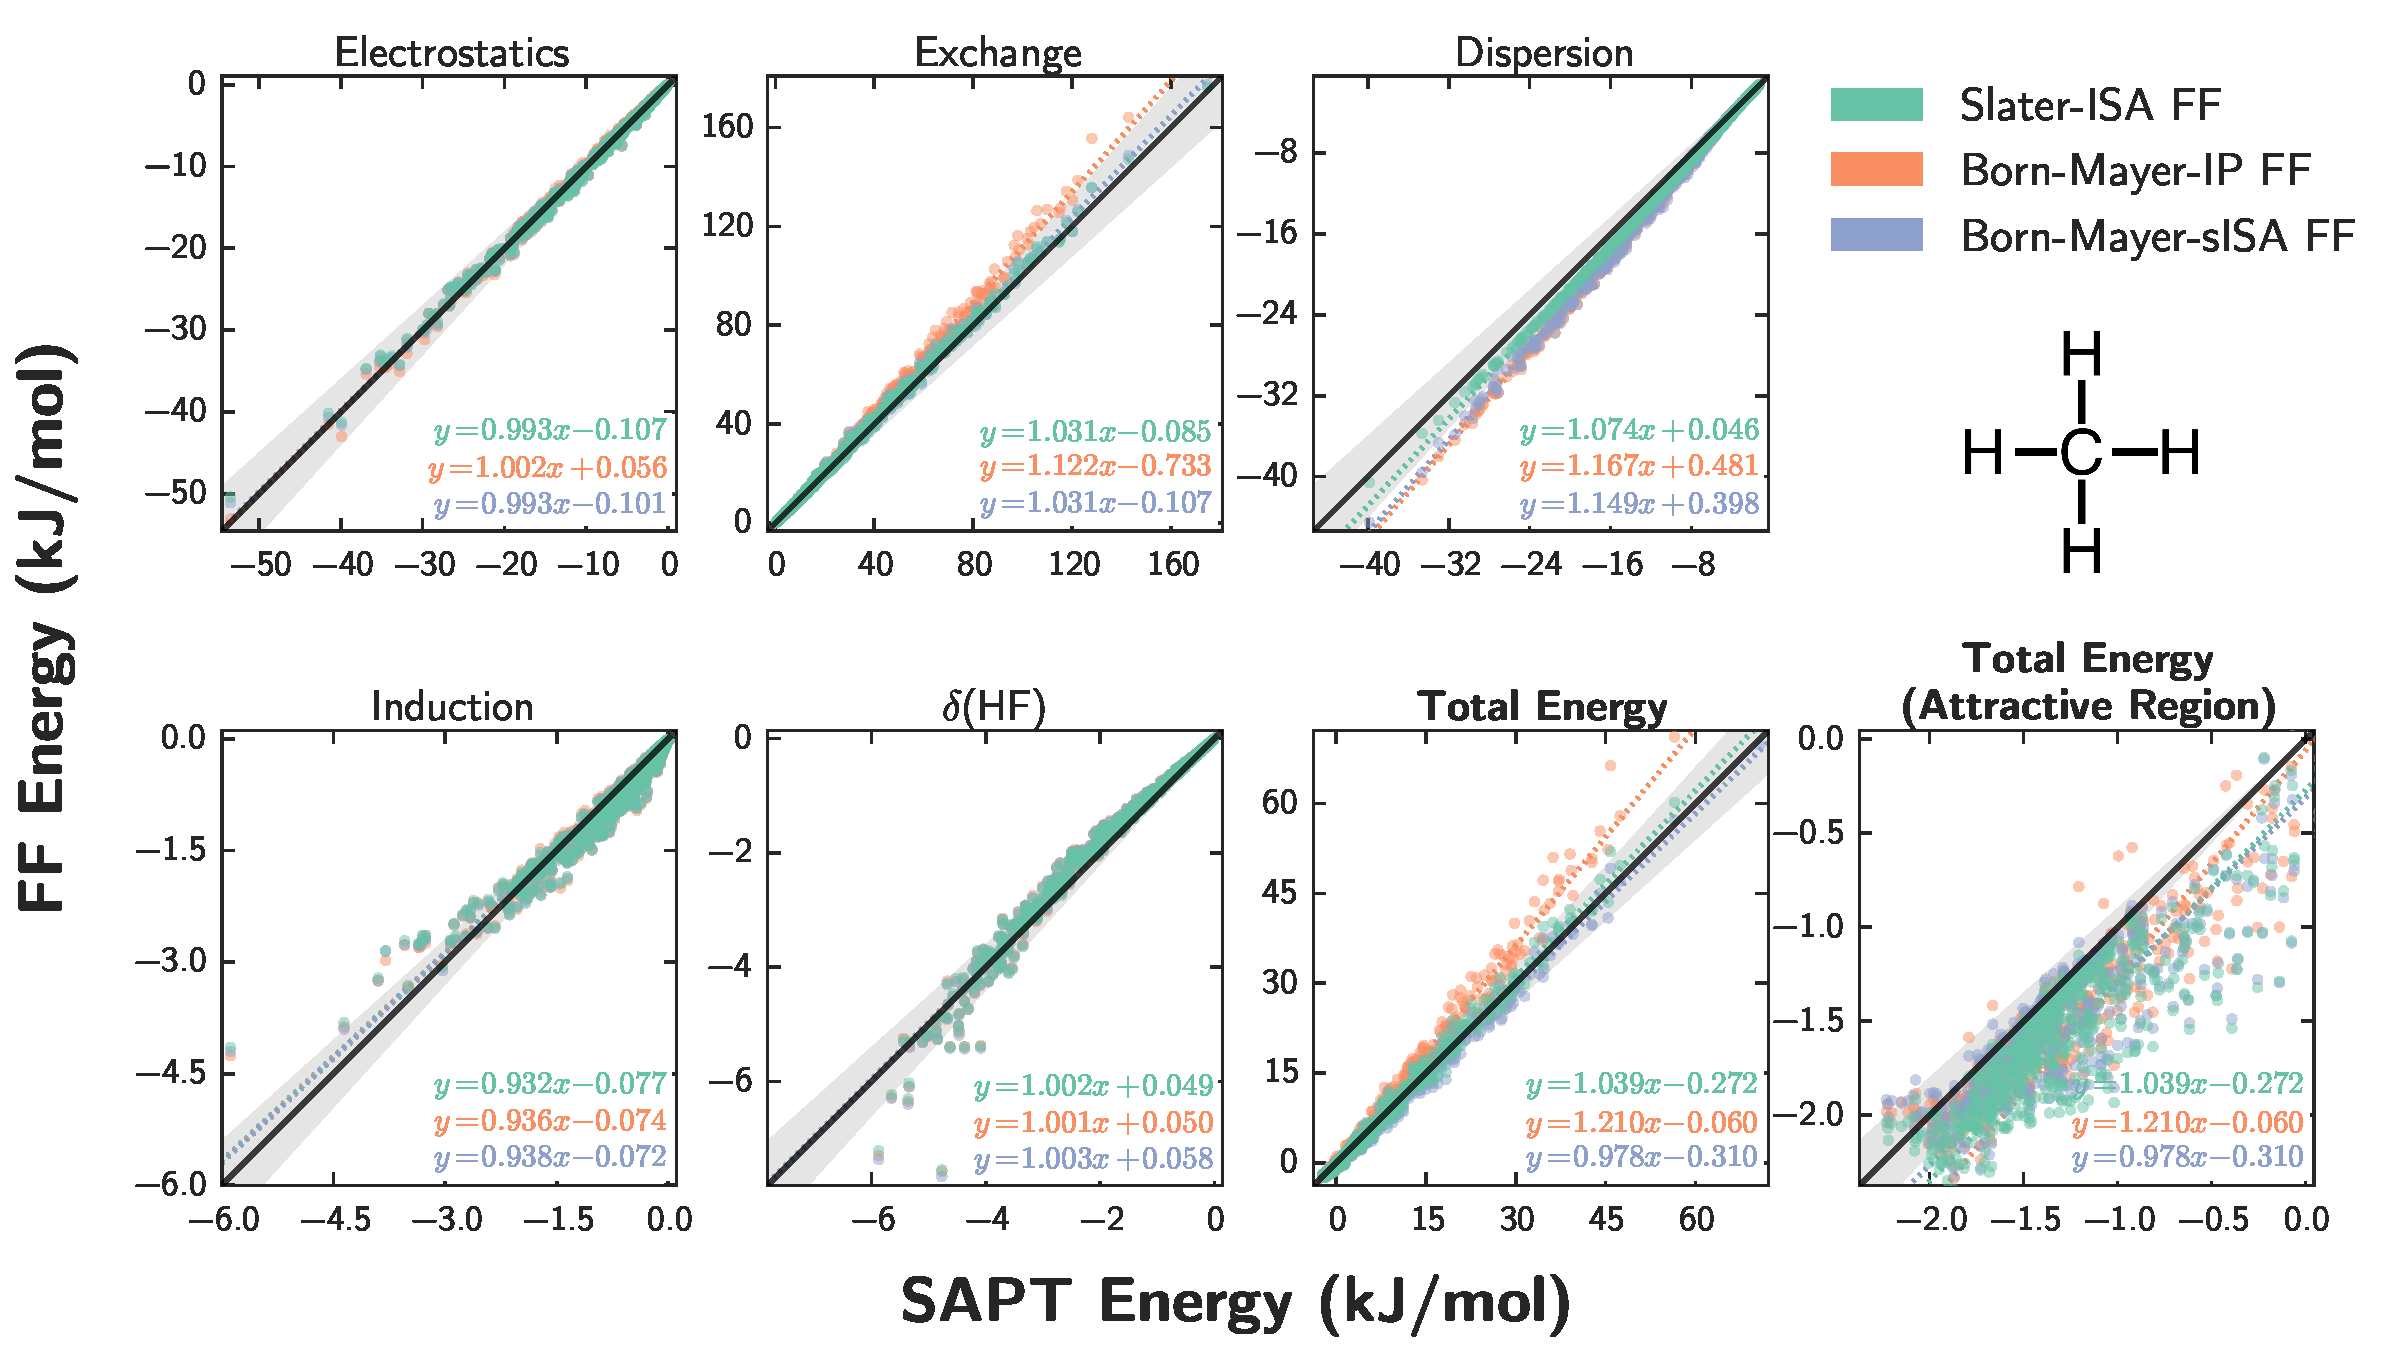
\includegraphics[width=0.9\textwidth]{isotropic/si/methane_methane_scatter.pdf}
    \end{subfigure}
    \end{figure}
    \begin{figure}
    \ContinuedFloat
    \begin{subfigure}{\textwidth}
        \caption{Methanol Dimer}
        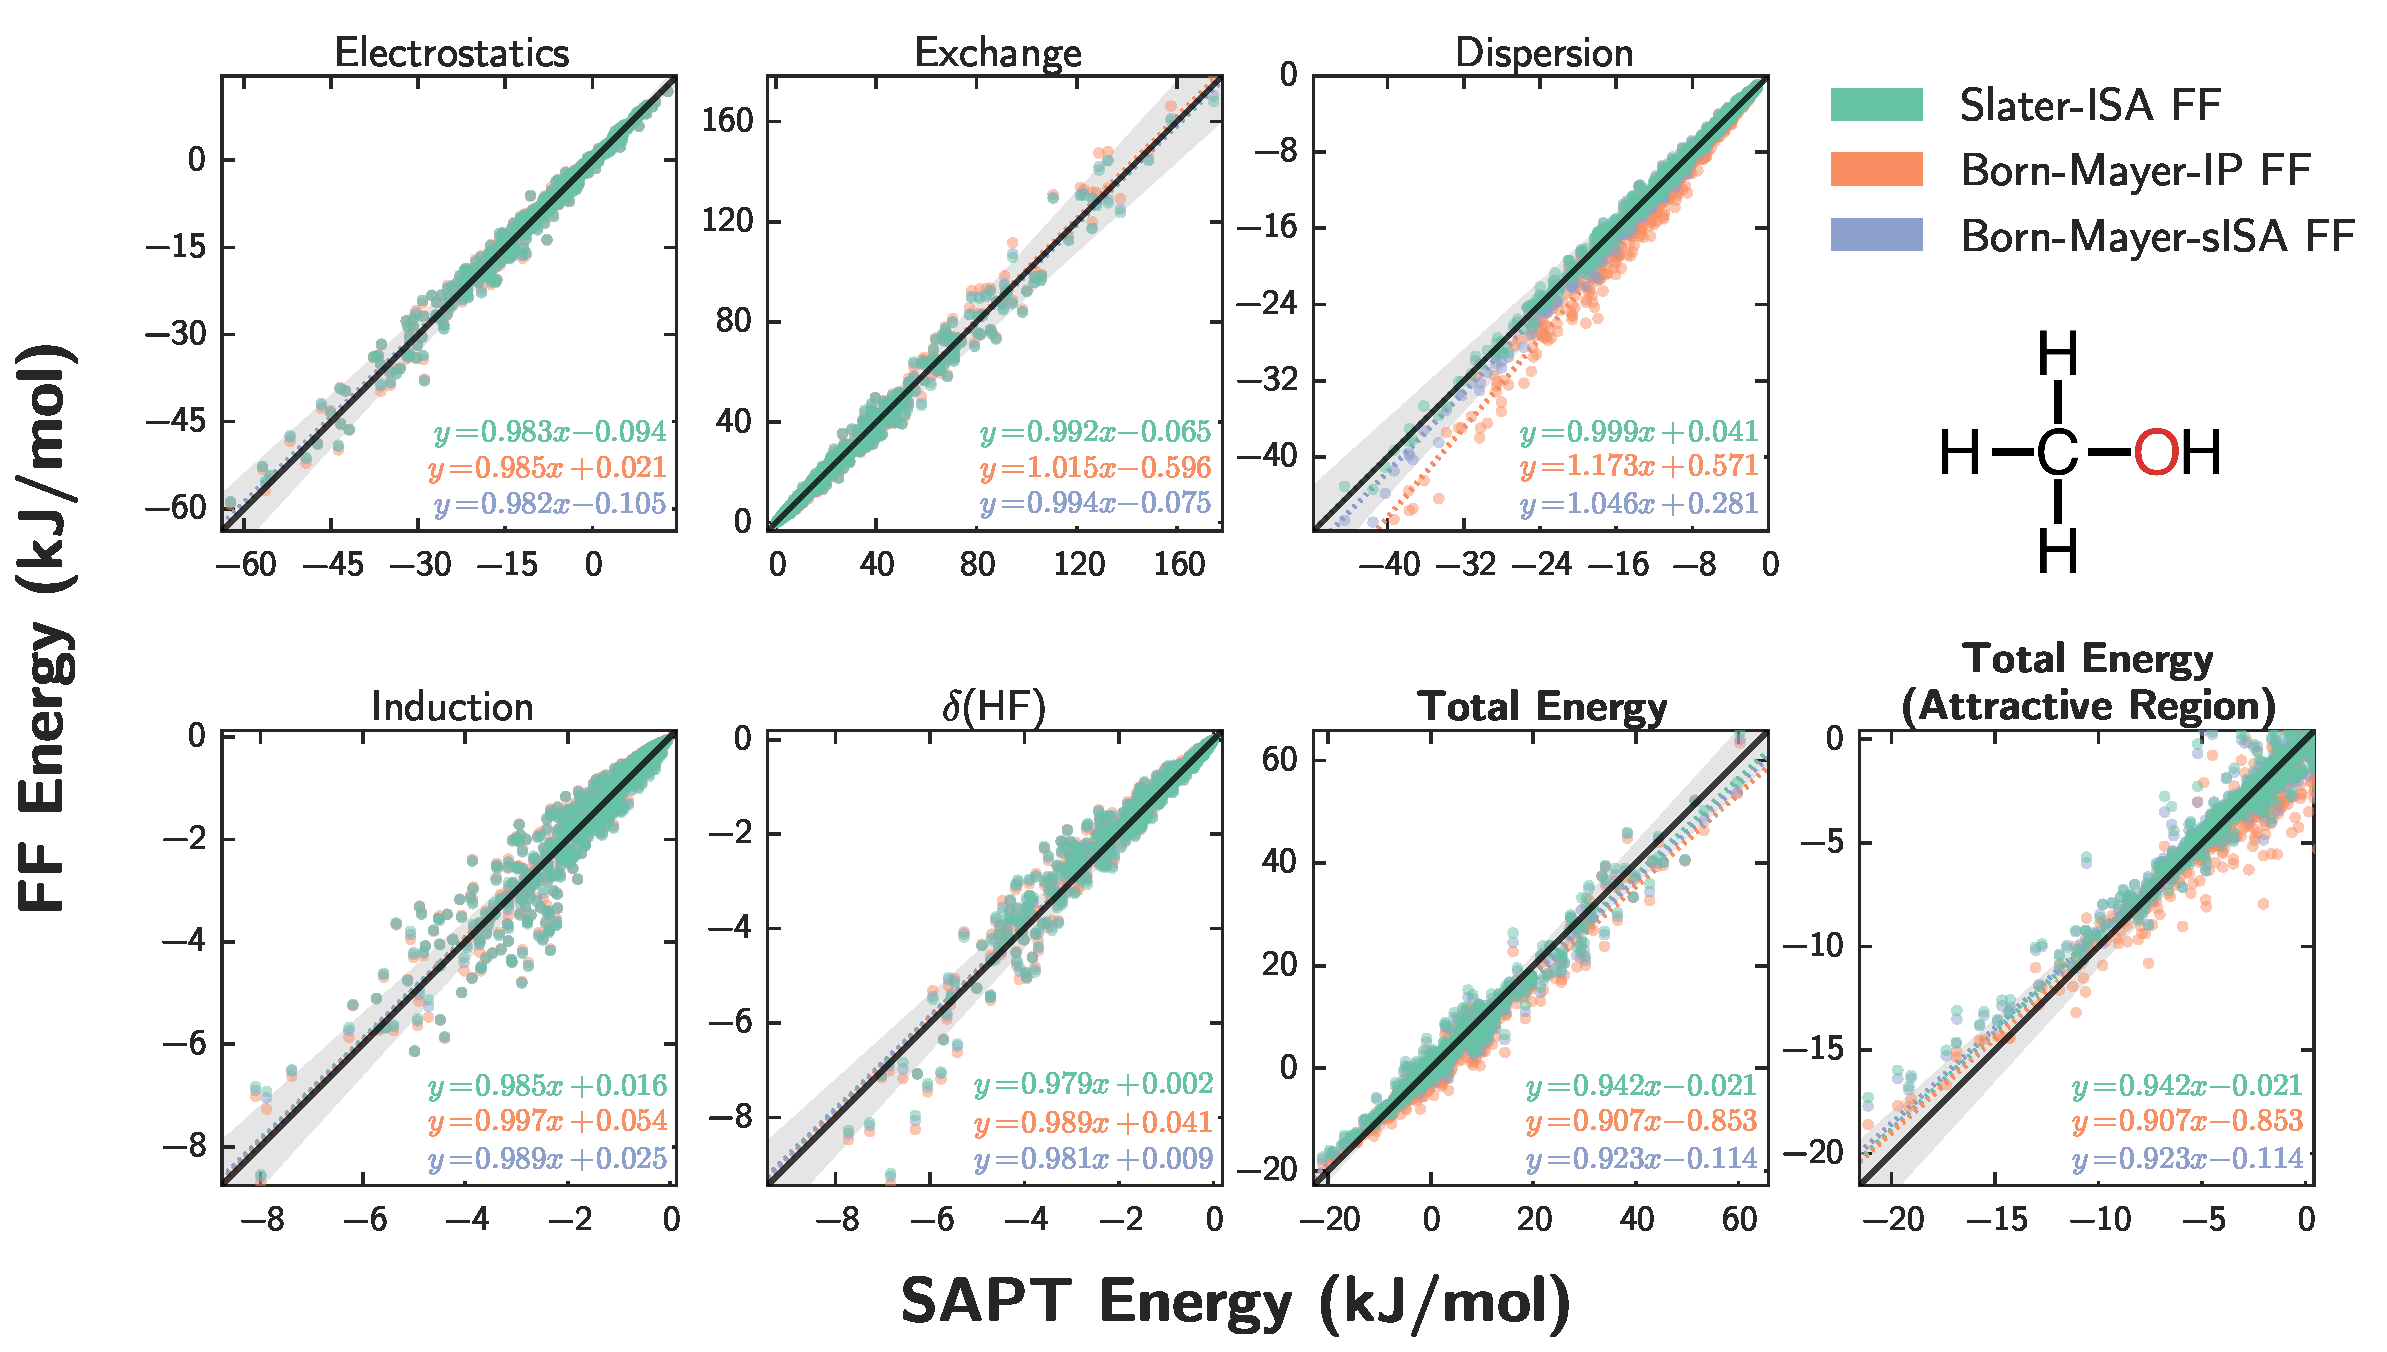
\includegraphics[width=0.9\textwidth]{isotropic/si/methanol_methanol_scatter.pdf}
    \end{subfigure}
    \begin{subfigure}{\textwidth}
        \caption{Methyl Amine Dimer}
        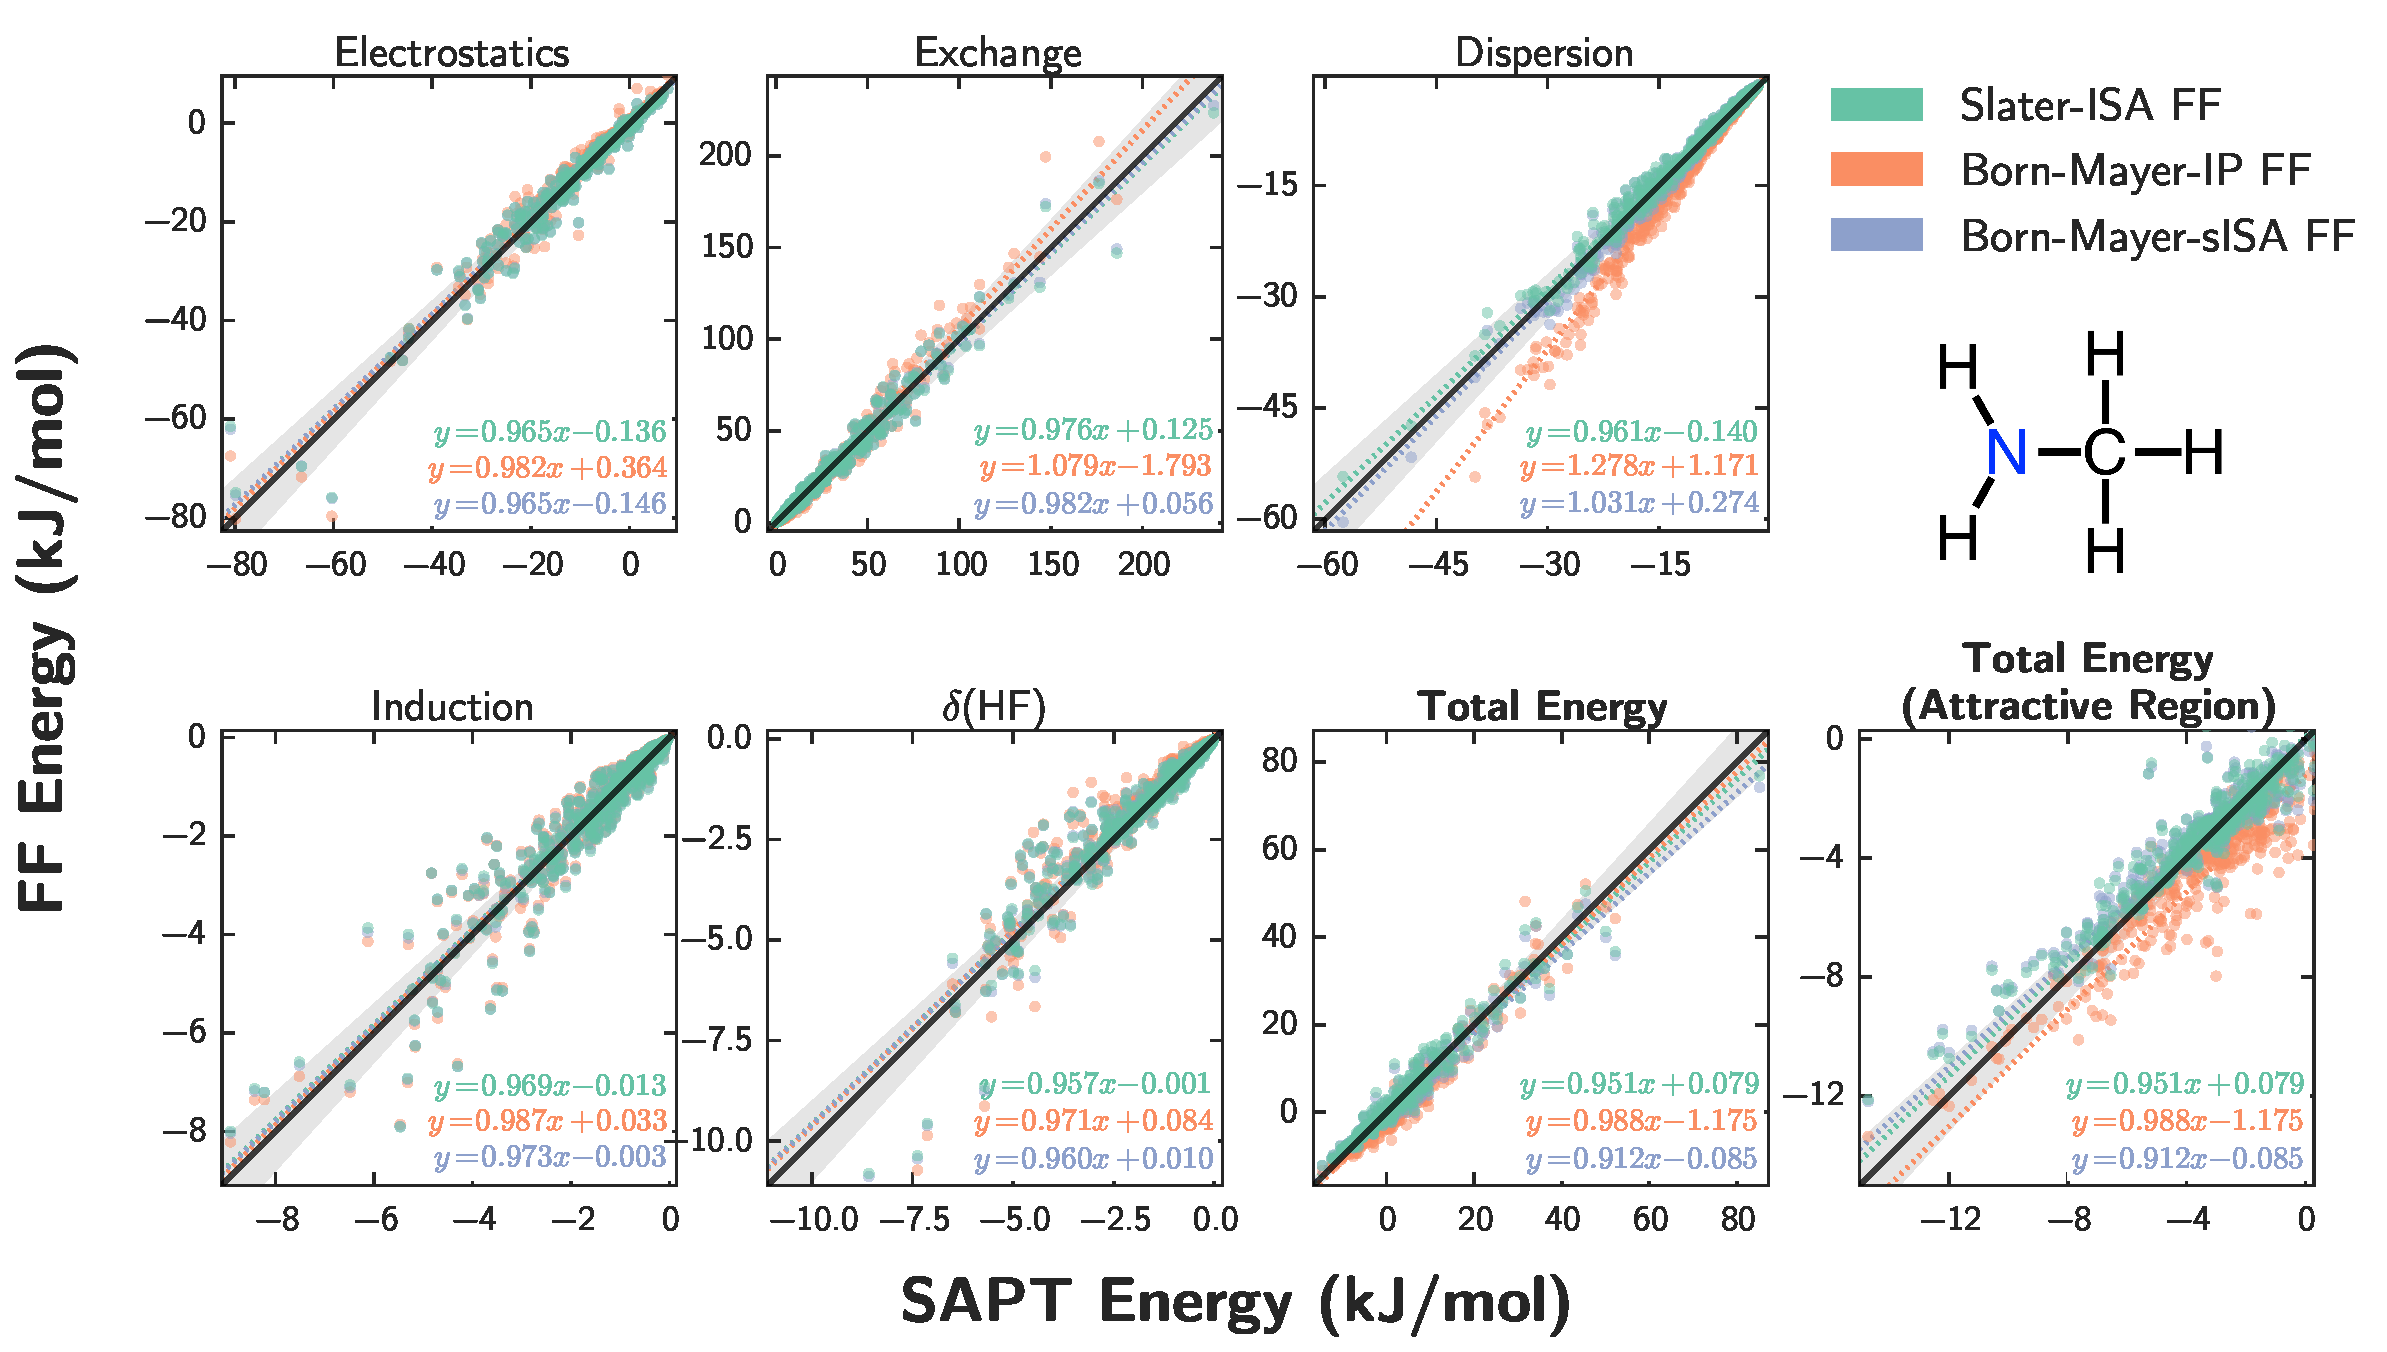
\includegraphics[width=0.9\textwidth]{isotropic/si/methyl_amine_methyl_amine_scatter.pdf}
    \end{subfigure}
    \end{figure}
    \begin{figure}
    \ContinuedFloat
    \begin{subfigure}{\textwidth}
        \caption{\nh Dimer}
        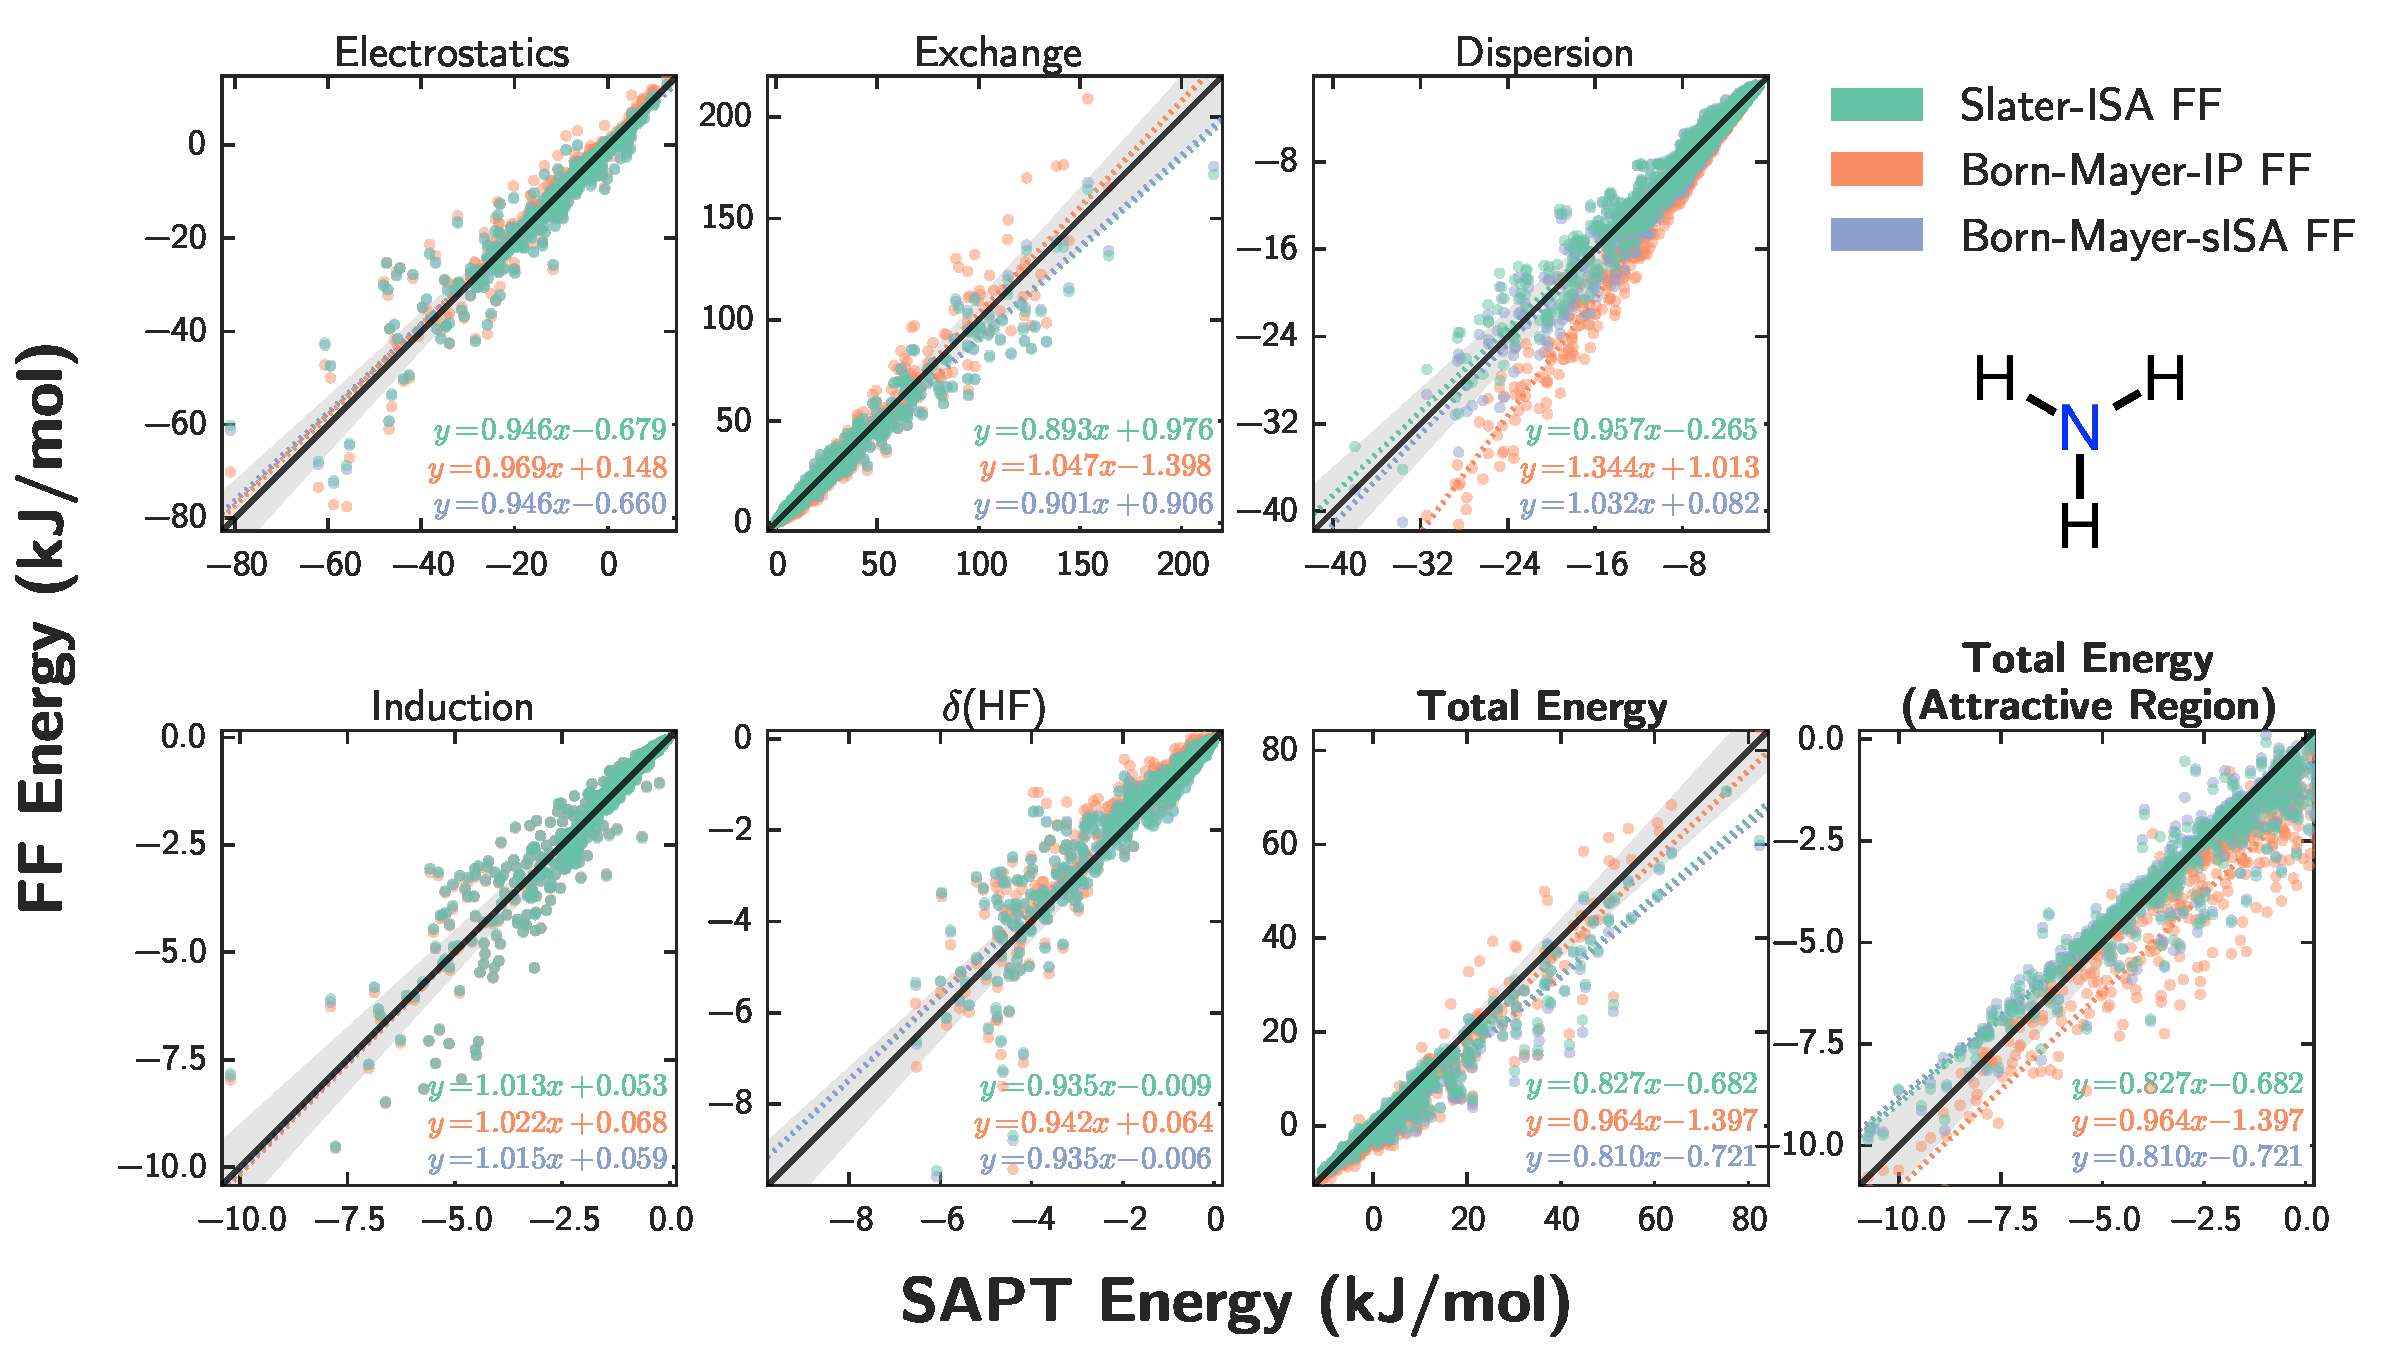
\includegraphics[width=0.9\textwidth]{isotropic/si/nh3_nh3_scatter.pdf}
    \end{subfigure}
    \caption{
    Force field fits for the homomoneric systems using the \isaffold (green), \saptff
(orange) and \bmsisaff (blue).
    Fits for each energy component are displayed along with two views of the total interaction energy.
    The $y=x$ line (black) indicates perfect agreement between reference energies
    and each force field, while shaded grey areas represent points within $\pm
    10\%$ agreement of the benchmark. To guide the eye, a line of best fit (dotted
    line) has been computed for each force field and for each energy component.
     }
    \label{fig:all-scatter}
    \end{figure}
    %%%%%%%% All Scatter %%%%%%%%%%






\end{section}
%% \clearpage
%% \begin{section}{Force Field Accuracy for \ljff}
%% 
%%     %%%%%%%%%%%% Ar-Ar PES %%%%%%%%%%%%%%%%%%
%%     \begin{figure}
%%     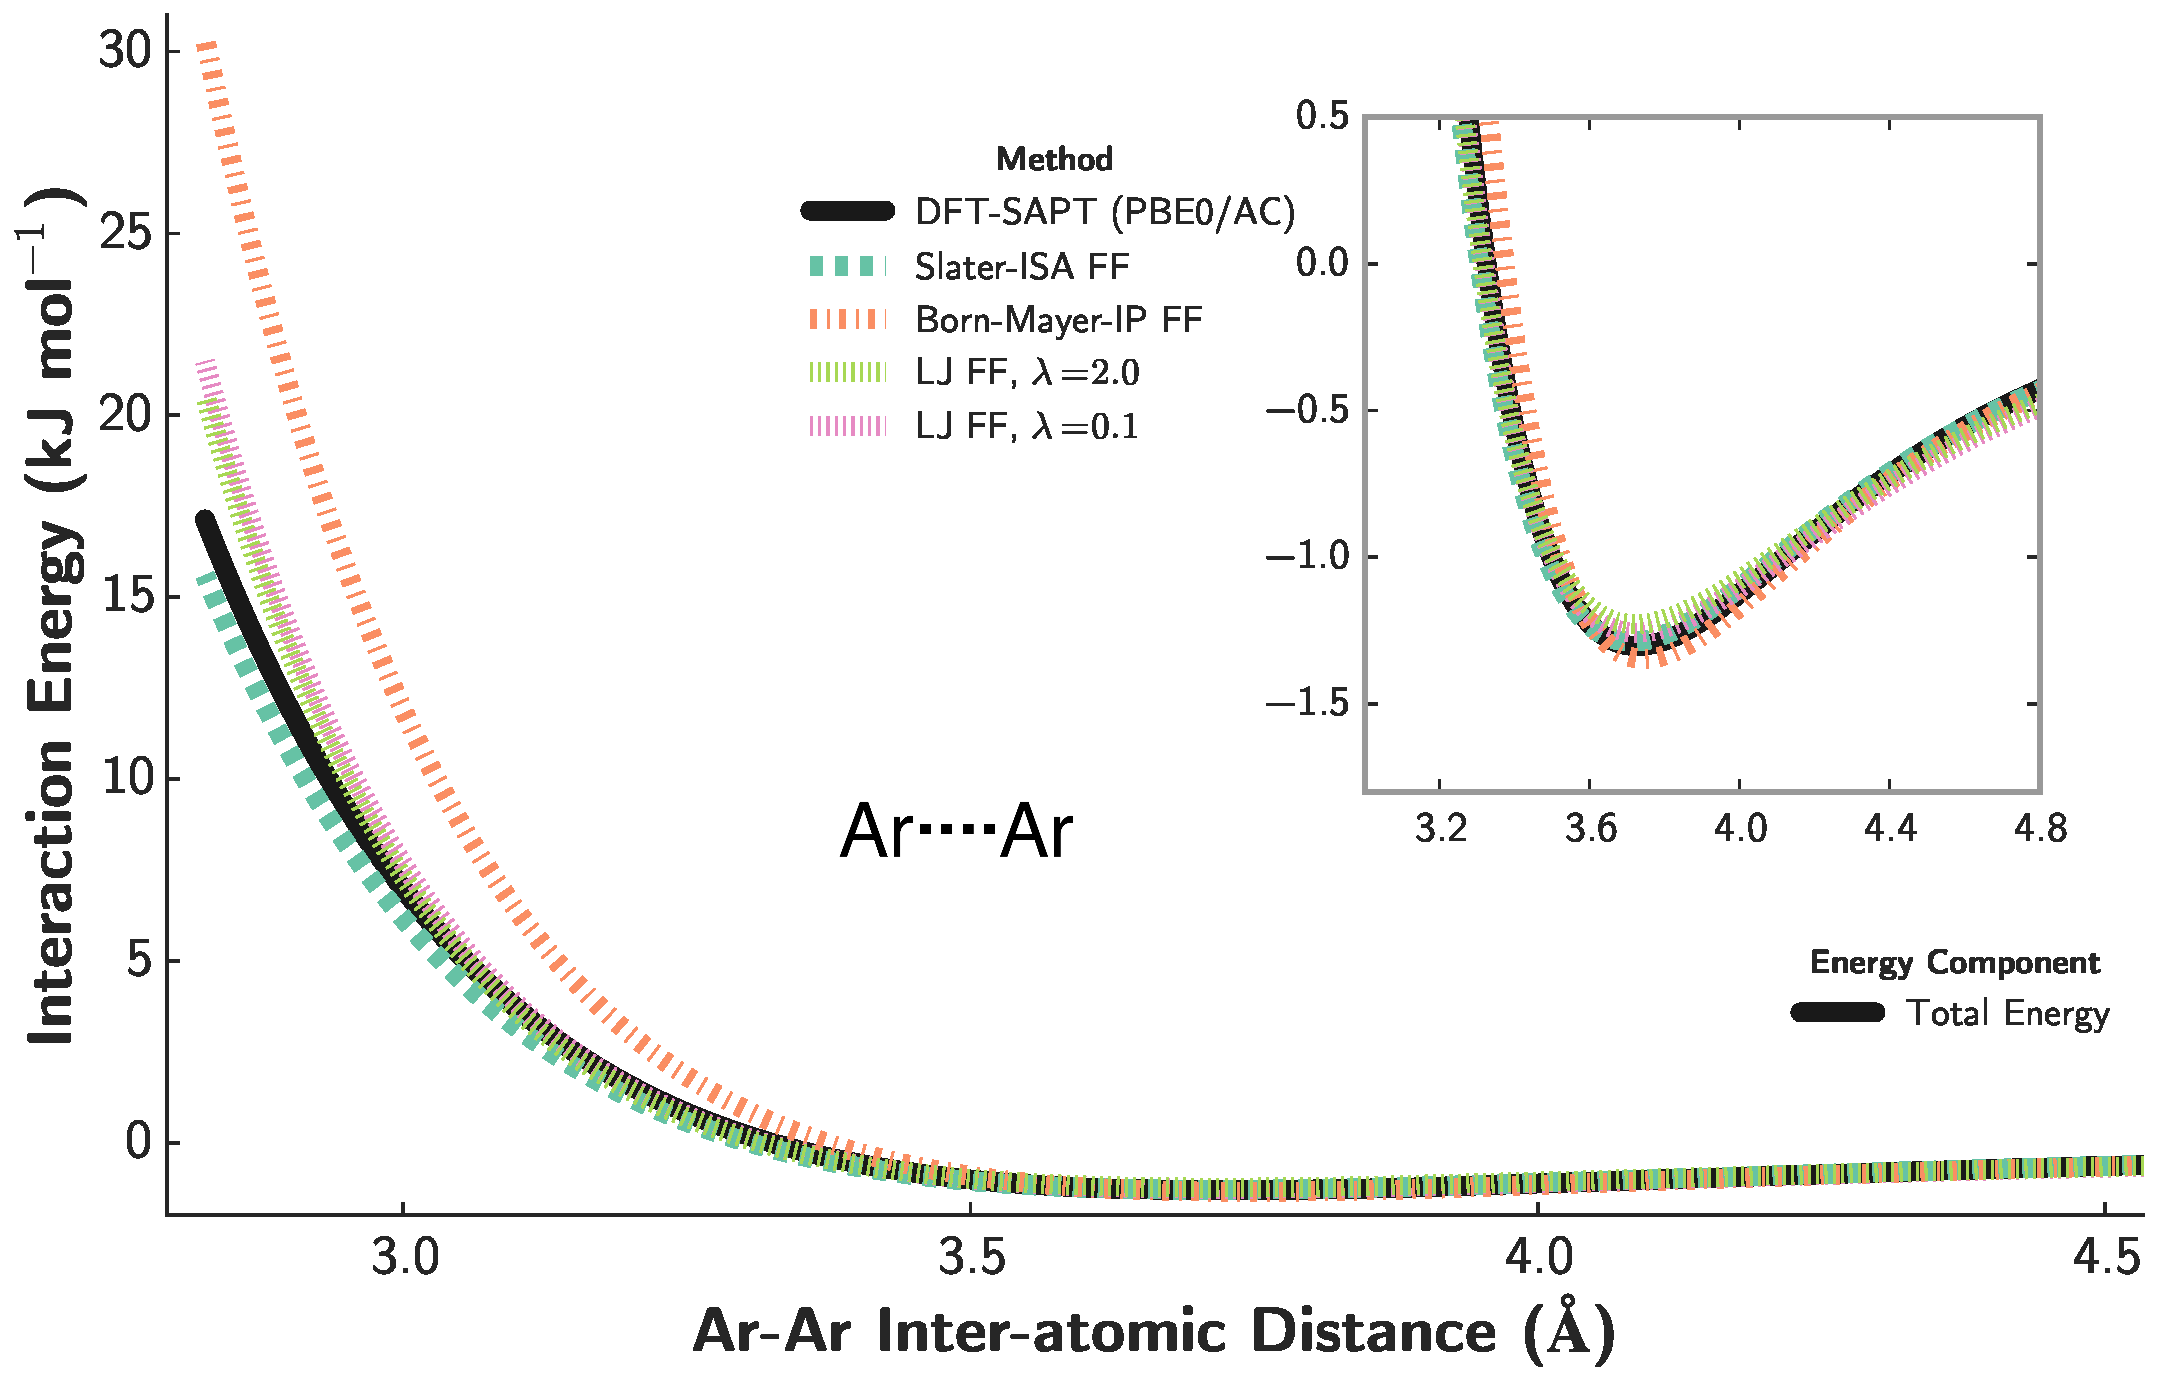
\includegraphics[width=0.9\textwidth]{isotropic/si/ar_ar_pes_wi_lj.pdf}
%%     \caption{
%%     Potential energy surface for the argon dimer. 
%%     Interaction energies for the \isaffold (dashed curves), \saptff (dash-dotted
%%     curves), and \ljff (dotted curves) are shown alongside benchmark \saptpbeo energies (solid curves). 
%%     Note that, for the \ljff force fields, 
%%     the magnitude of the attractive tail region is overestimated by the
%%     effective $C_{ij,6}$ dispersion parameter.
%%     }
%%     \label{fig:ar-pes}
%%     \end{figure}
%%     %%%%%%%%%%%% Ar-Ar PES %%%%%%%%%%%%%%%%%%
%% 
%% 
%%     %%%%%%%% Ethane-Ethane Scatter %%%%%%%%%%
%%     \begin{figure}
%%     %\includegraphics[width=0.9\textwidth]{isotropic/si/ammonia_ff_quality.png}
%%     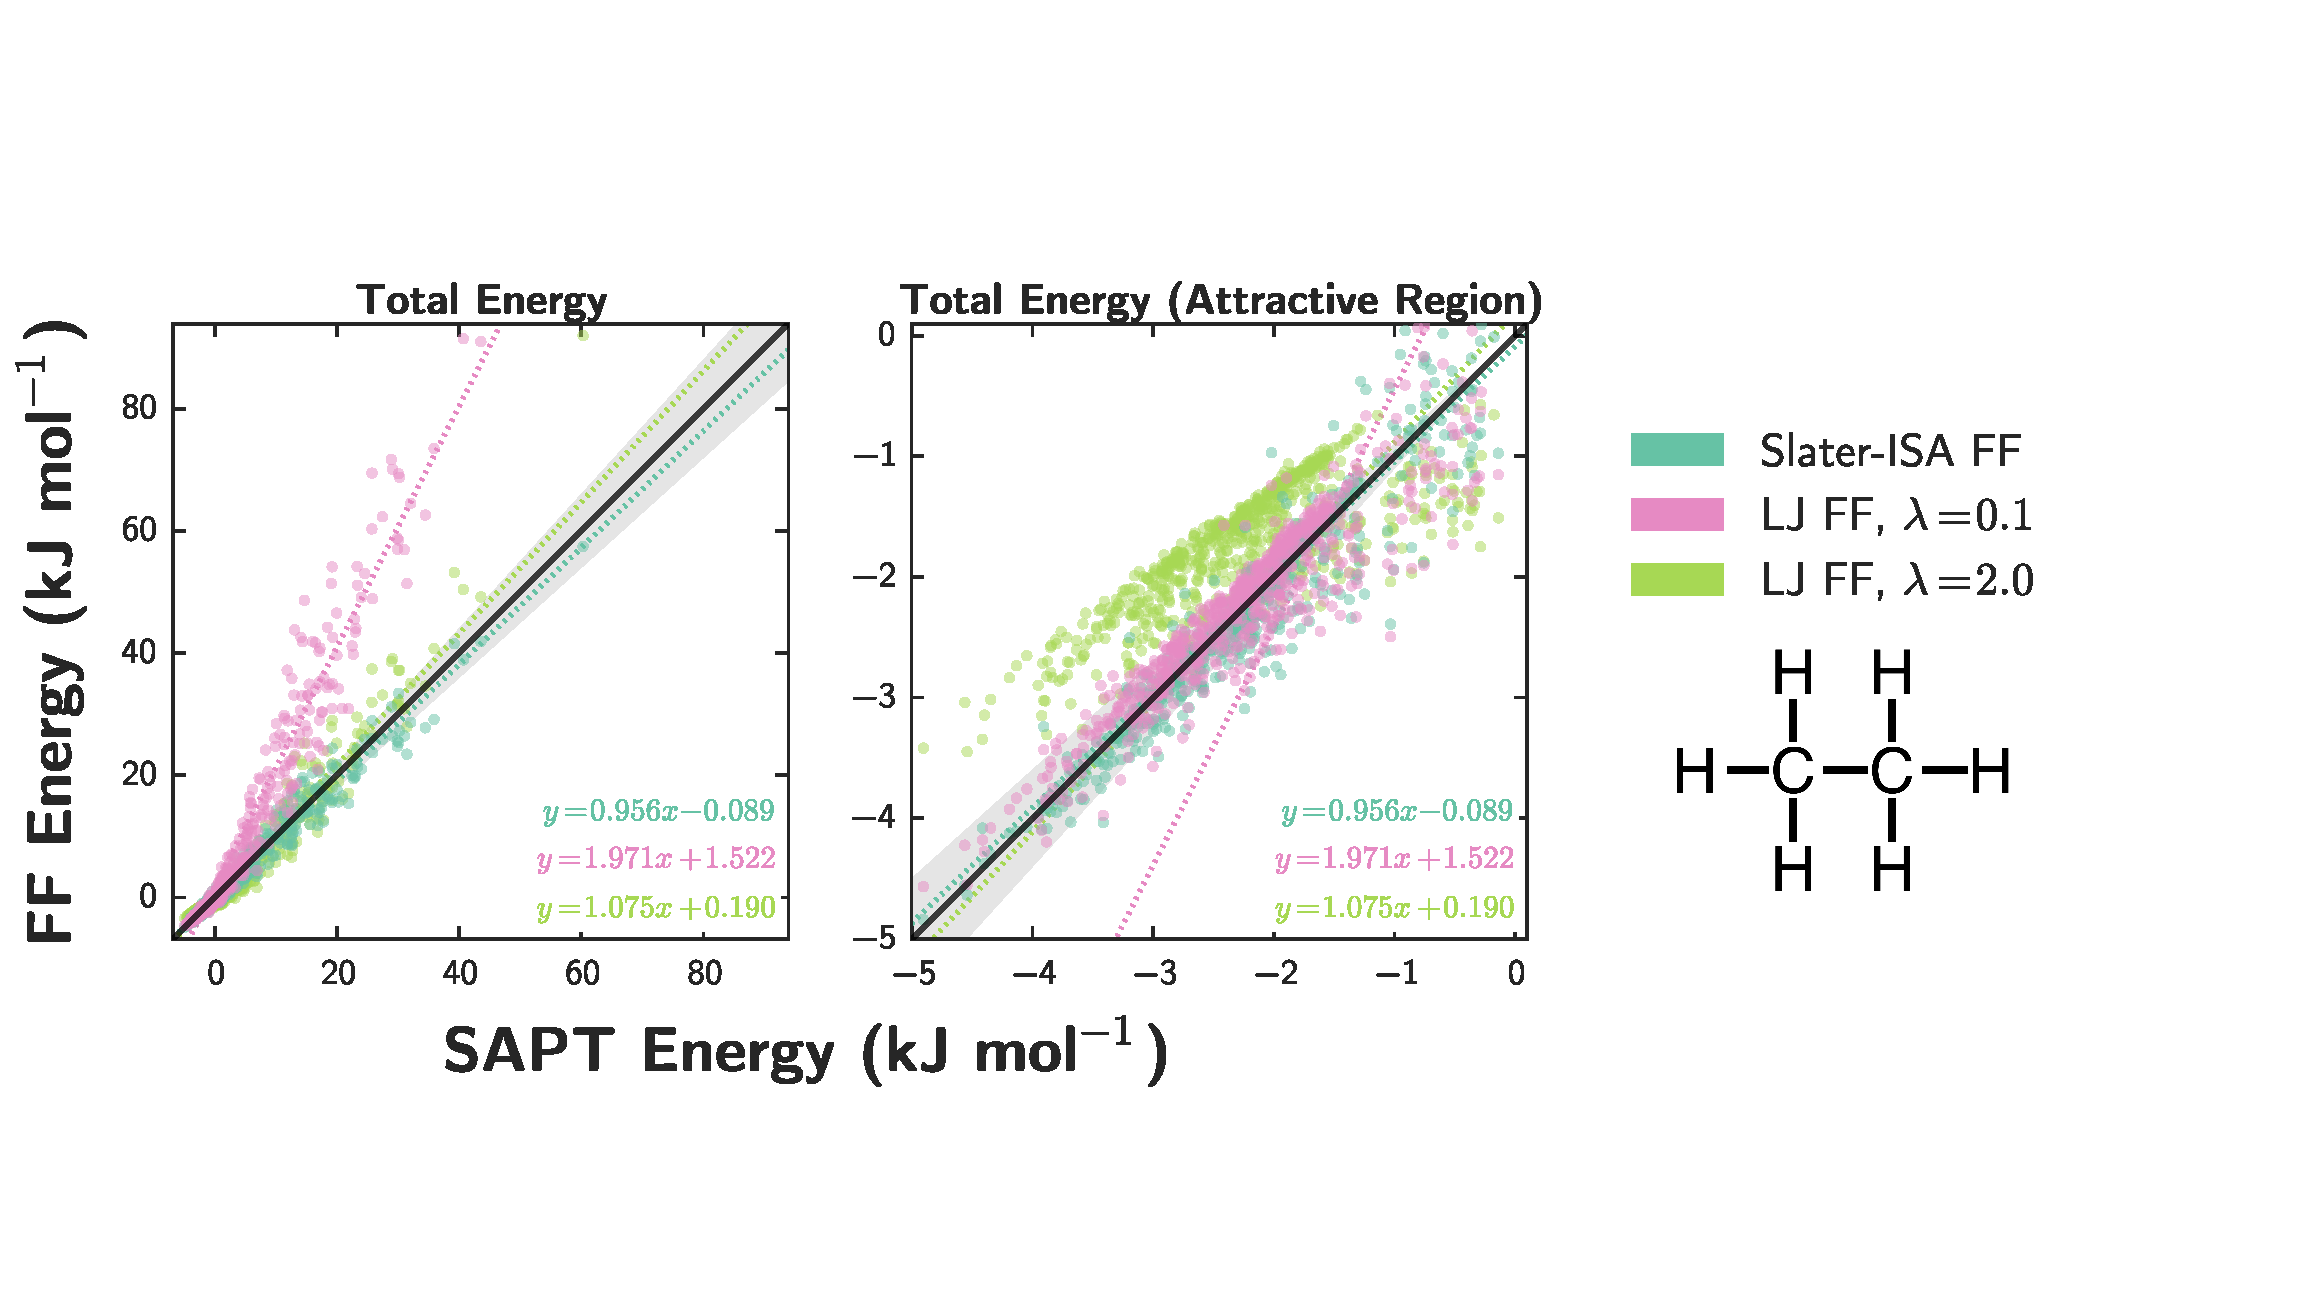
\includegraphics[width=0.9\textwidth]{isotropic/si/ethane_ethane_lj_scatter.pdf}
%%     \caption[foo]{
%%     Fits for two views of the total interaction energy for 
%%     the ethane dimer using the Slater-ISA (teal),
%%     LJ $\lambda = 0.1$ (pink) and LJ $\lambda = 2.0$ (lime green) FFs.
%%     The diagonal line (black) indicates perfect agreement between reference energies
%%     and each force field, while shaded grey areas represent points within $\pm
%%     10\%$ agreement of the benchmark. To guide the eye, a line of best fit (dotted
%%     line) has been computed for each force field.
%%      }
%%     \label{fig:ethane-scatter}
%%     \end{figure}
%%     %%%%%%%% Ethane-Ethane Scatter %%%%%%%%%%
%% 
%%     %%%%%%%%%%% Ethane-Ethane PES %%%%%%%%%%%
%%     \begin{figure}
%%     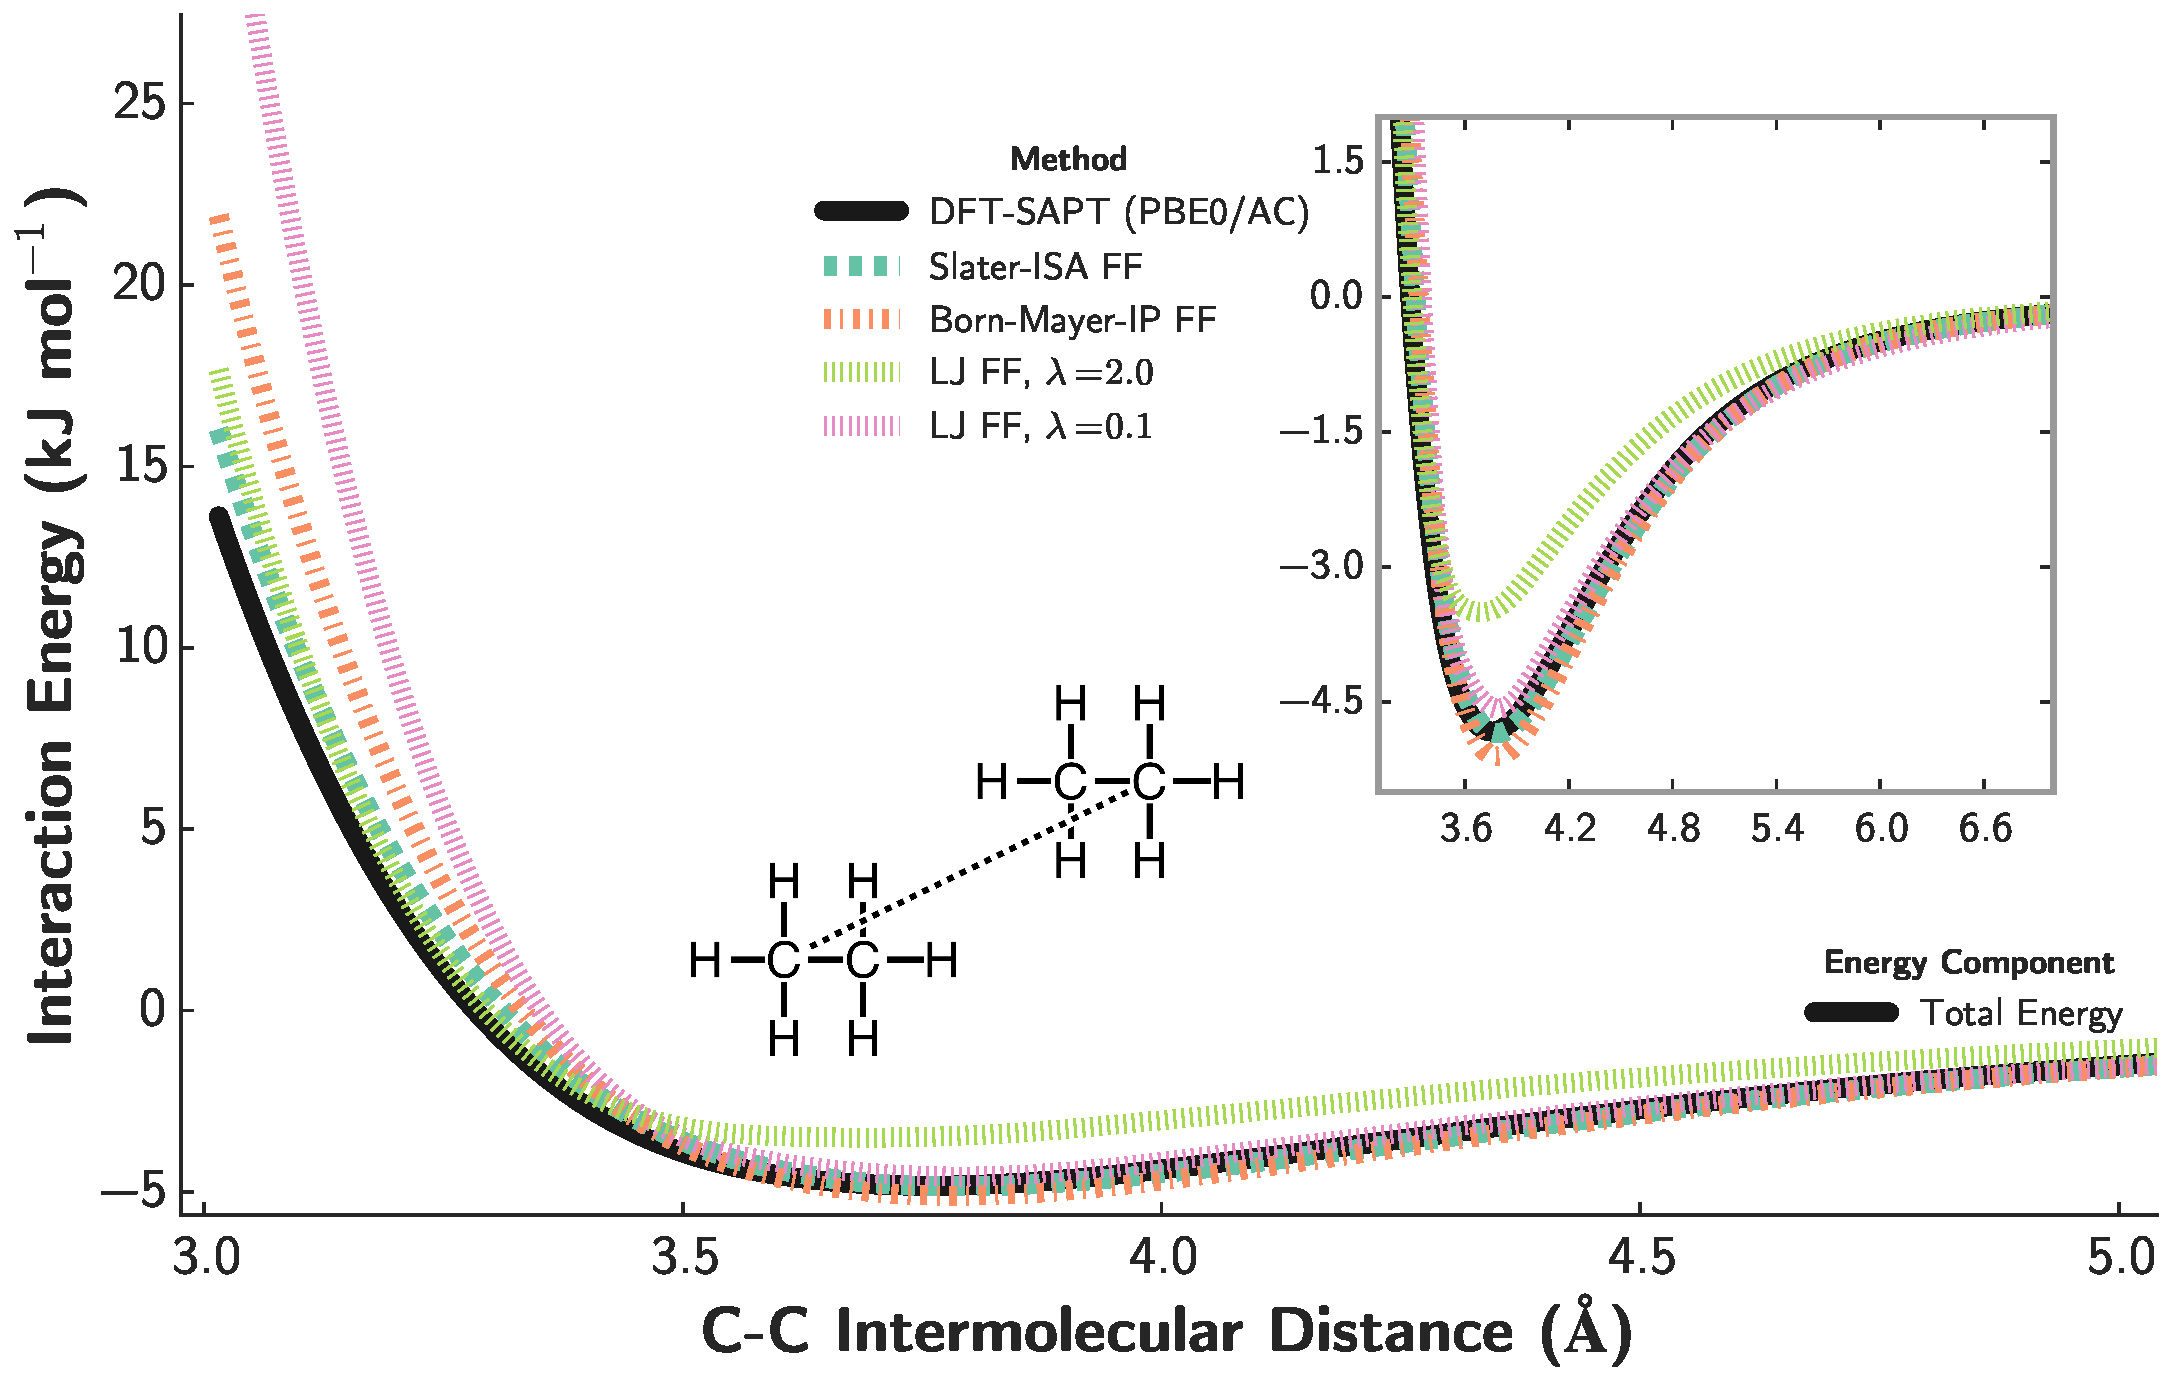
\includegraphics[width=0.9\textwidth]{isotropic/si/ethane_ethane_pes_wi_lj.pdf}
%%     \caption{
%%     A representative potential energy scan near a local minimum for the ethane dimer. 
%%     Interaction energies for the \isaffold (dashed curves), \saptff (dash-dotted
%%     curves), and \ljff (dotted curves)  are shown alongside benchmark \saptpbeo energies (solid curves). The
%%     energy decomposition for DFT-SAPT and for each force field is shown for reference.
%%      The ethane dimer configuration in this scan corresponds to the most
%%     energetically attractive dimer included in the training set; other
%%     points along this scan are not included in the training set.
%%     }
%%     \label{fig:ethane-pes}
%%     \end{figure}
%%     %%%%%%%%%%% Ethane-Ethane PES %%%%%%%%%%%
%% 
%%     %%%%%%%% Acetone-Acetone Scatter %%%%%%%%%%
%%     \begin{figure}
%%     %\includegraphics[width=0.9\textwidth]{isotropic/si/ammonia_ff_quality.png}
%%     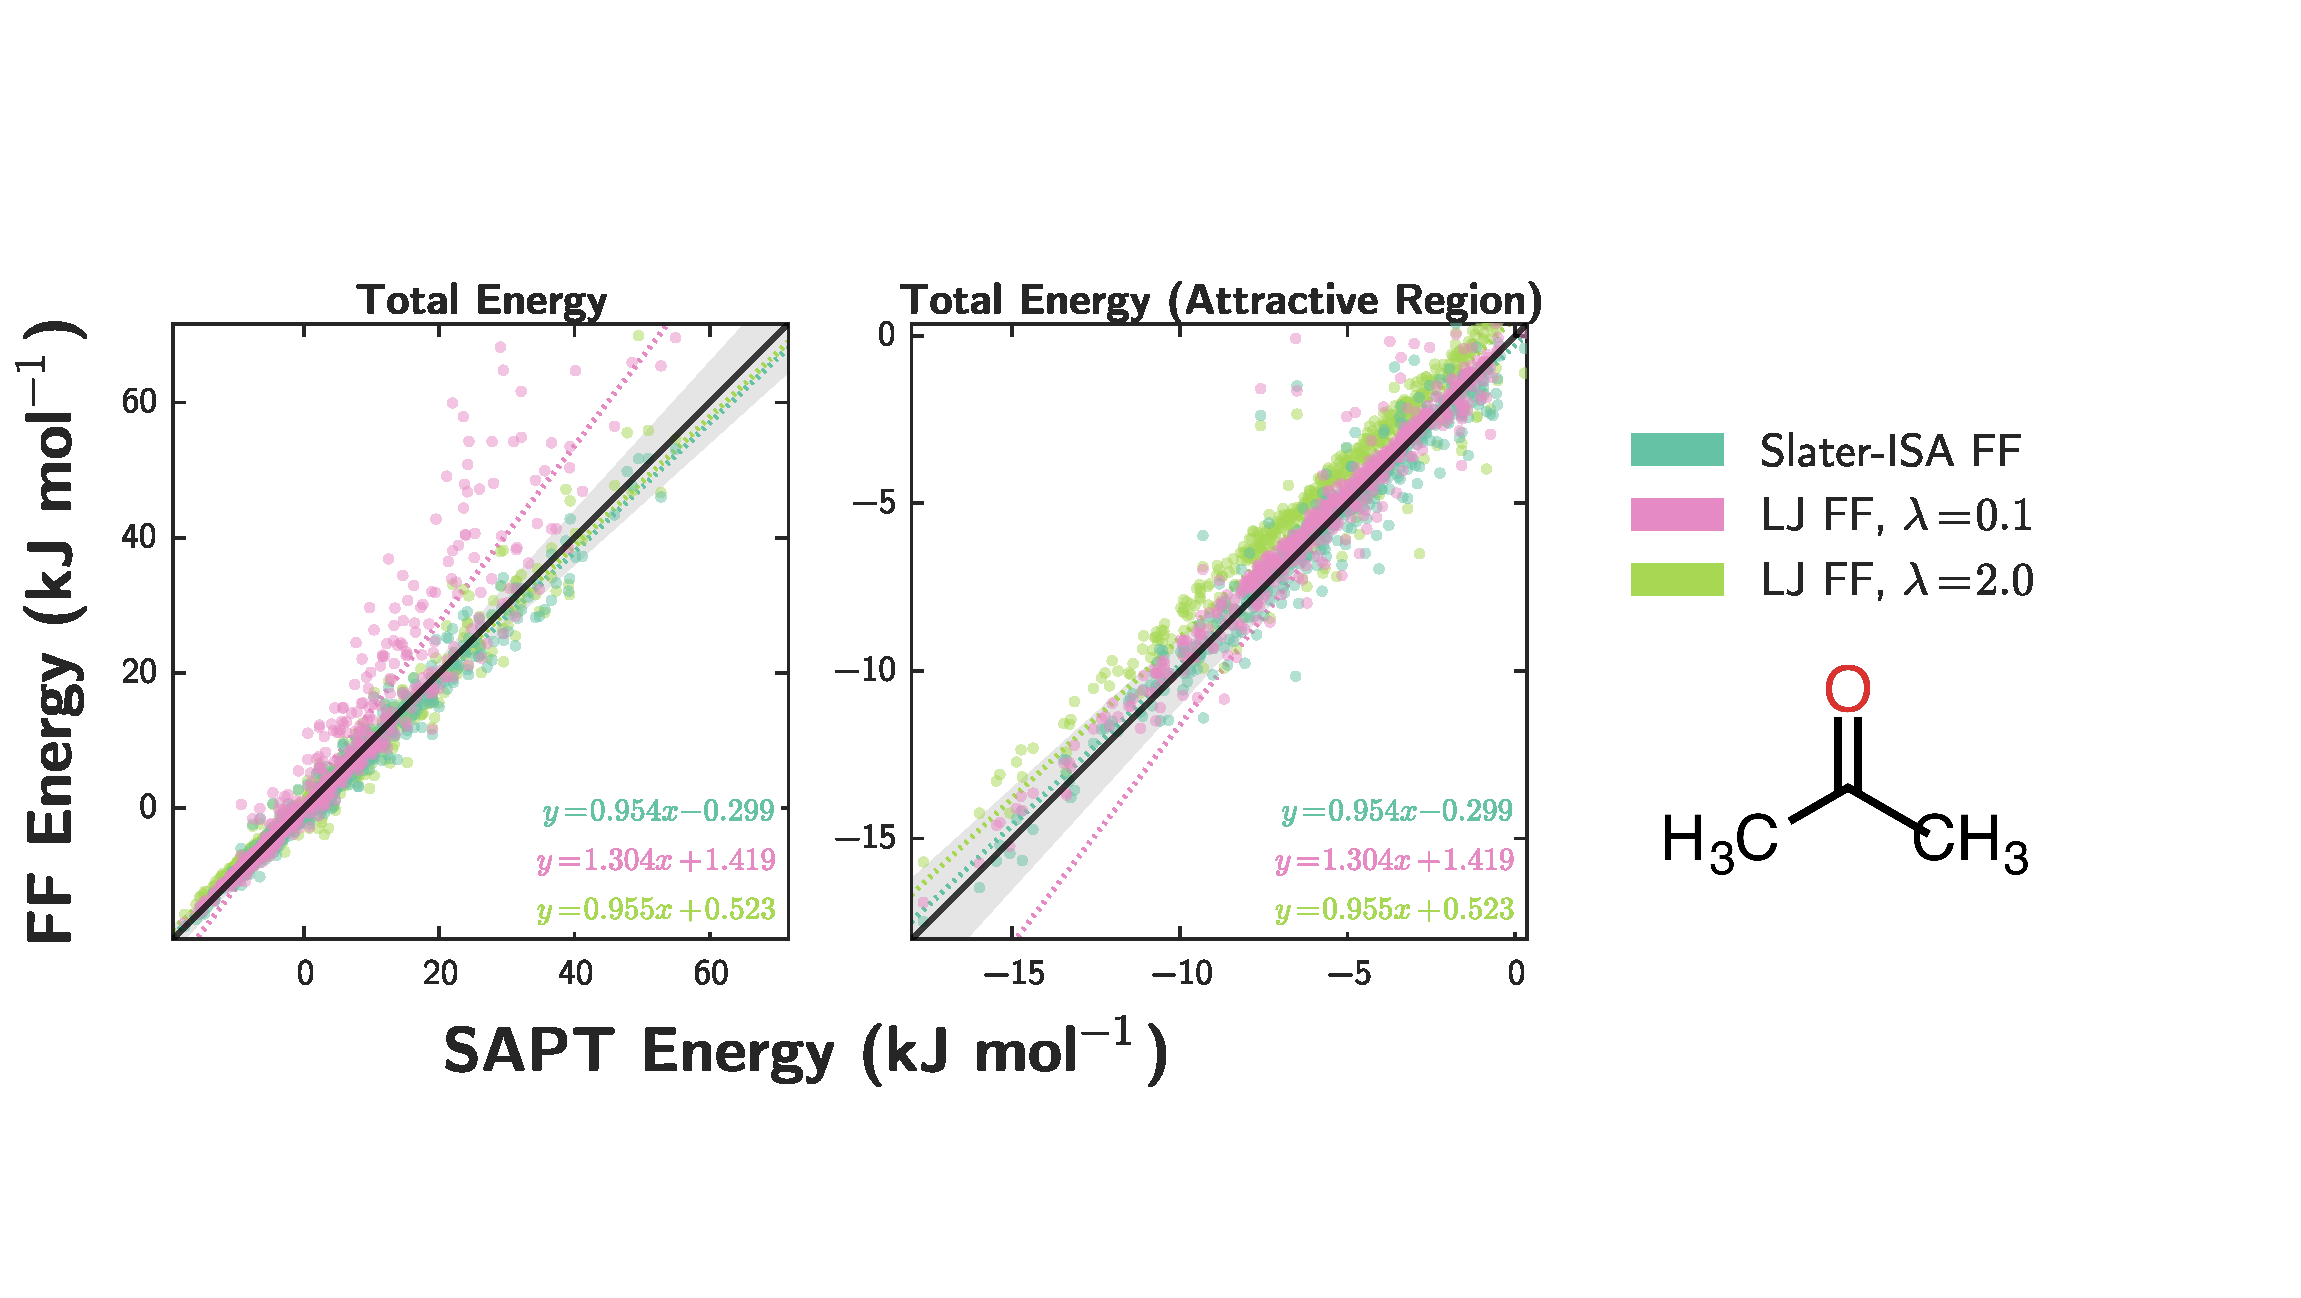
\includegraphics[width=0.9\textwidth]{isotropic/si/acetone_acetone_lj_scatter.pdf}
%%     \caption{
%%     Force field fits for the acetone dimer using the Slater-ISA (teal), LJ
%% $\lambda = 0.1$ (pink) and LJ $\lambda = 2.0$ (lime green) FFs.
%%     Fits for two views of the total interaction energy are displayed.
%%     The diagonal line (black) indicates perfect agreement between reference energies
%%     and each force field, while shaded grey areas represent points within $\pm
%%     10\%$ agreement of the benchmark. To guide the eye, a line of best fit (dotted
%%     line) has been computed for each force field.
%%      }
%%     \label{fig:acetone-scatter}
%%     \end{figure}
%%     %%%%%%%% Acetone-Acetone Scatter %%%%%%%%%%
%% 
%%     %%%%%%%%%%% Acetone-Acetone PES %%%%%%%%%%%
%%     \begin{figure}
%%     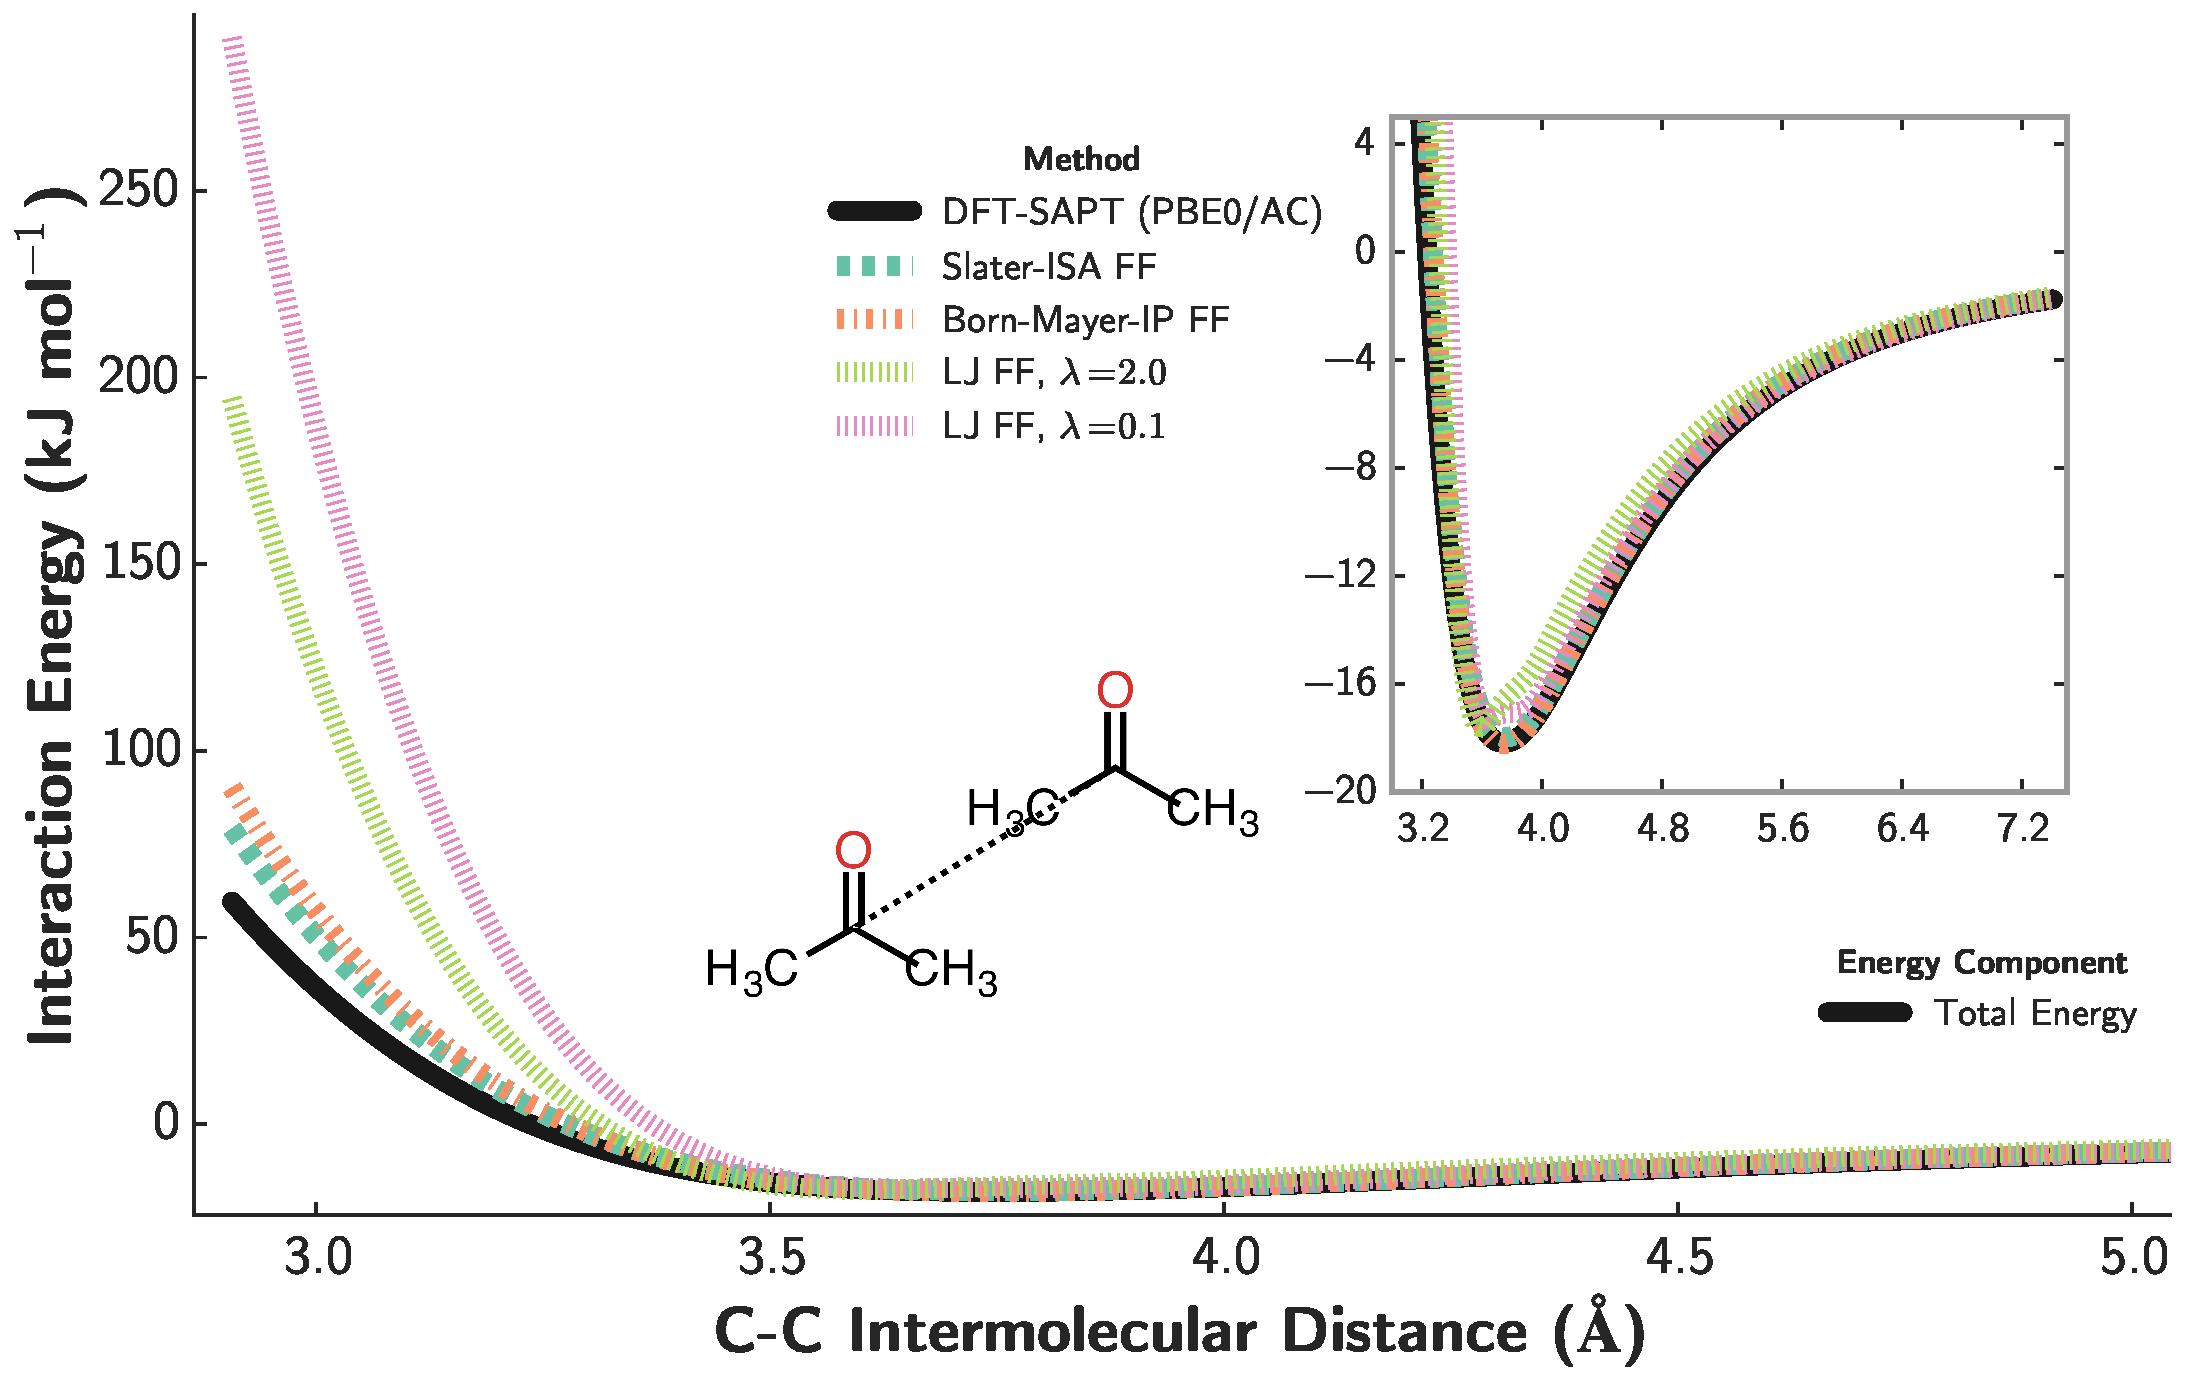
\includegraphics[width=0.9\textwidth]{isotropic/si/acetone_acetone_pes_wi_lj.pdf}
%%     \caption{
%%     A representative potential energy scan near a local minimum for the acetone dimer. 
%%     Interaction energies for the \isaffold (dashed curves), \saptff (dash-dotted
%%     curves), and \ljff (dotted curves) are shown alongside benchmark \saptpbeo energies (solid curves). The
%%     energy decomposition for DFT-SAPT and for each force field is shown for reference.
%%       The intermolecular distance is taken to be the
%%       internuclear distance between the two carbonyl carbons on each acetone
%%       monomer.  
%%      The acetone dimer configuration in this scan corresponds to the most
%%     energetically attractive dimer included in the training set; other
%%     points along this scan are not included in the training set.
%%     }
%%     \label{fig:acetone-pes}
%%     \end{figure}
%%     %%%%%%%%%%% Acetone-Acetone PES %%%%%%%%%%%
%% 
%% 
%% \end{section}
%% \clearpage
%% \begin{section}{Parameter Robustness for Argon}
%% 
%% Argon parameters were tested for robustness by changing the weighting function
%% as described in the main text. As with ethane, optimized \isaffold \A parameters are
%% much less sensitive to the choice of weighting function compared to
%% the \saptff. As a result, the \isaffold shows decreased uncertainty when computing
%% the 2\super{nd} virial coefficient. Virial coefficients for the \saptff, on the
%% other hand, depend more strongly on the choice of weighting function. The
%% fortuitous agreement with experiment for the \saptff with $\lambda = 0.5$ may
%% point to inaccuracies in the DFT-SAPT potential itself, but is not indicative of
%% enhanced force field fitting quality. (Indeed,
%% \ref{fig:ar-weighting} shows that this weighting function leads to the worst
%% agreement with DFT-SAPT compared to other $\lambda$ values). Overall, the
%% argon fits demonstrate increased parameter robustness for the \isaffold.
%% 
%% 
%%     %%%%%%%% Weighting Function Tests %%%%%%%
%%     \begin{figure}
%%     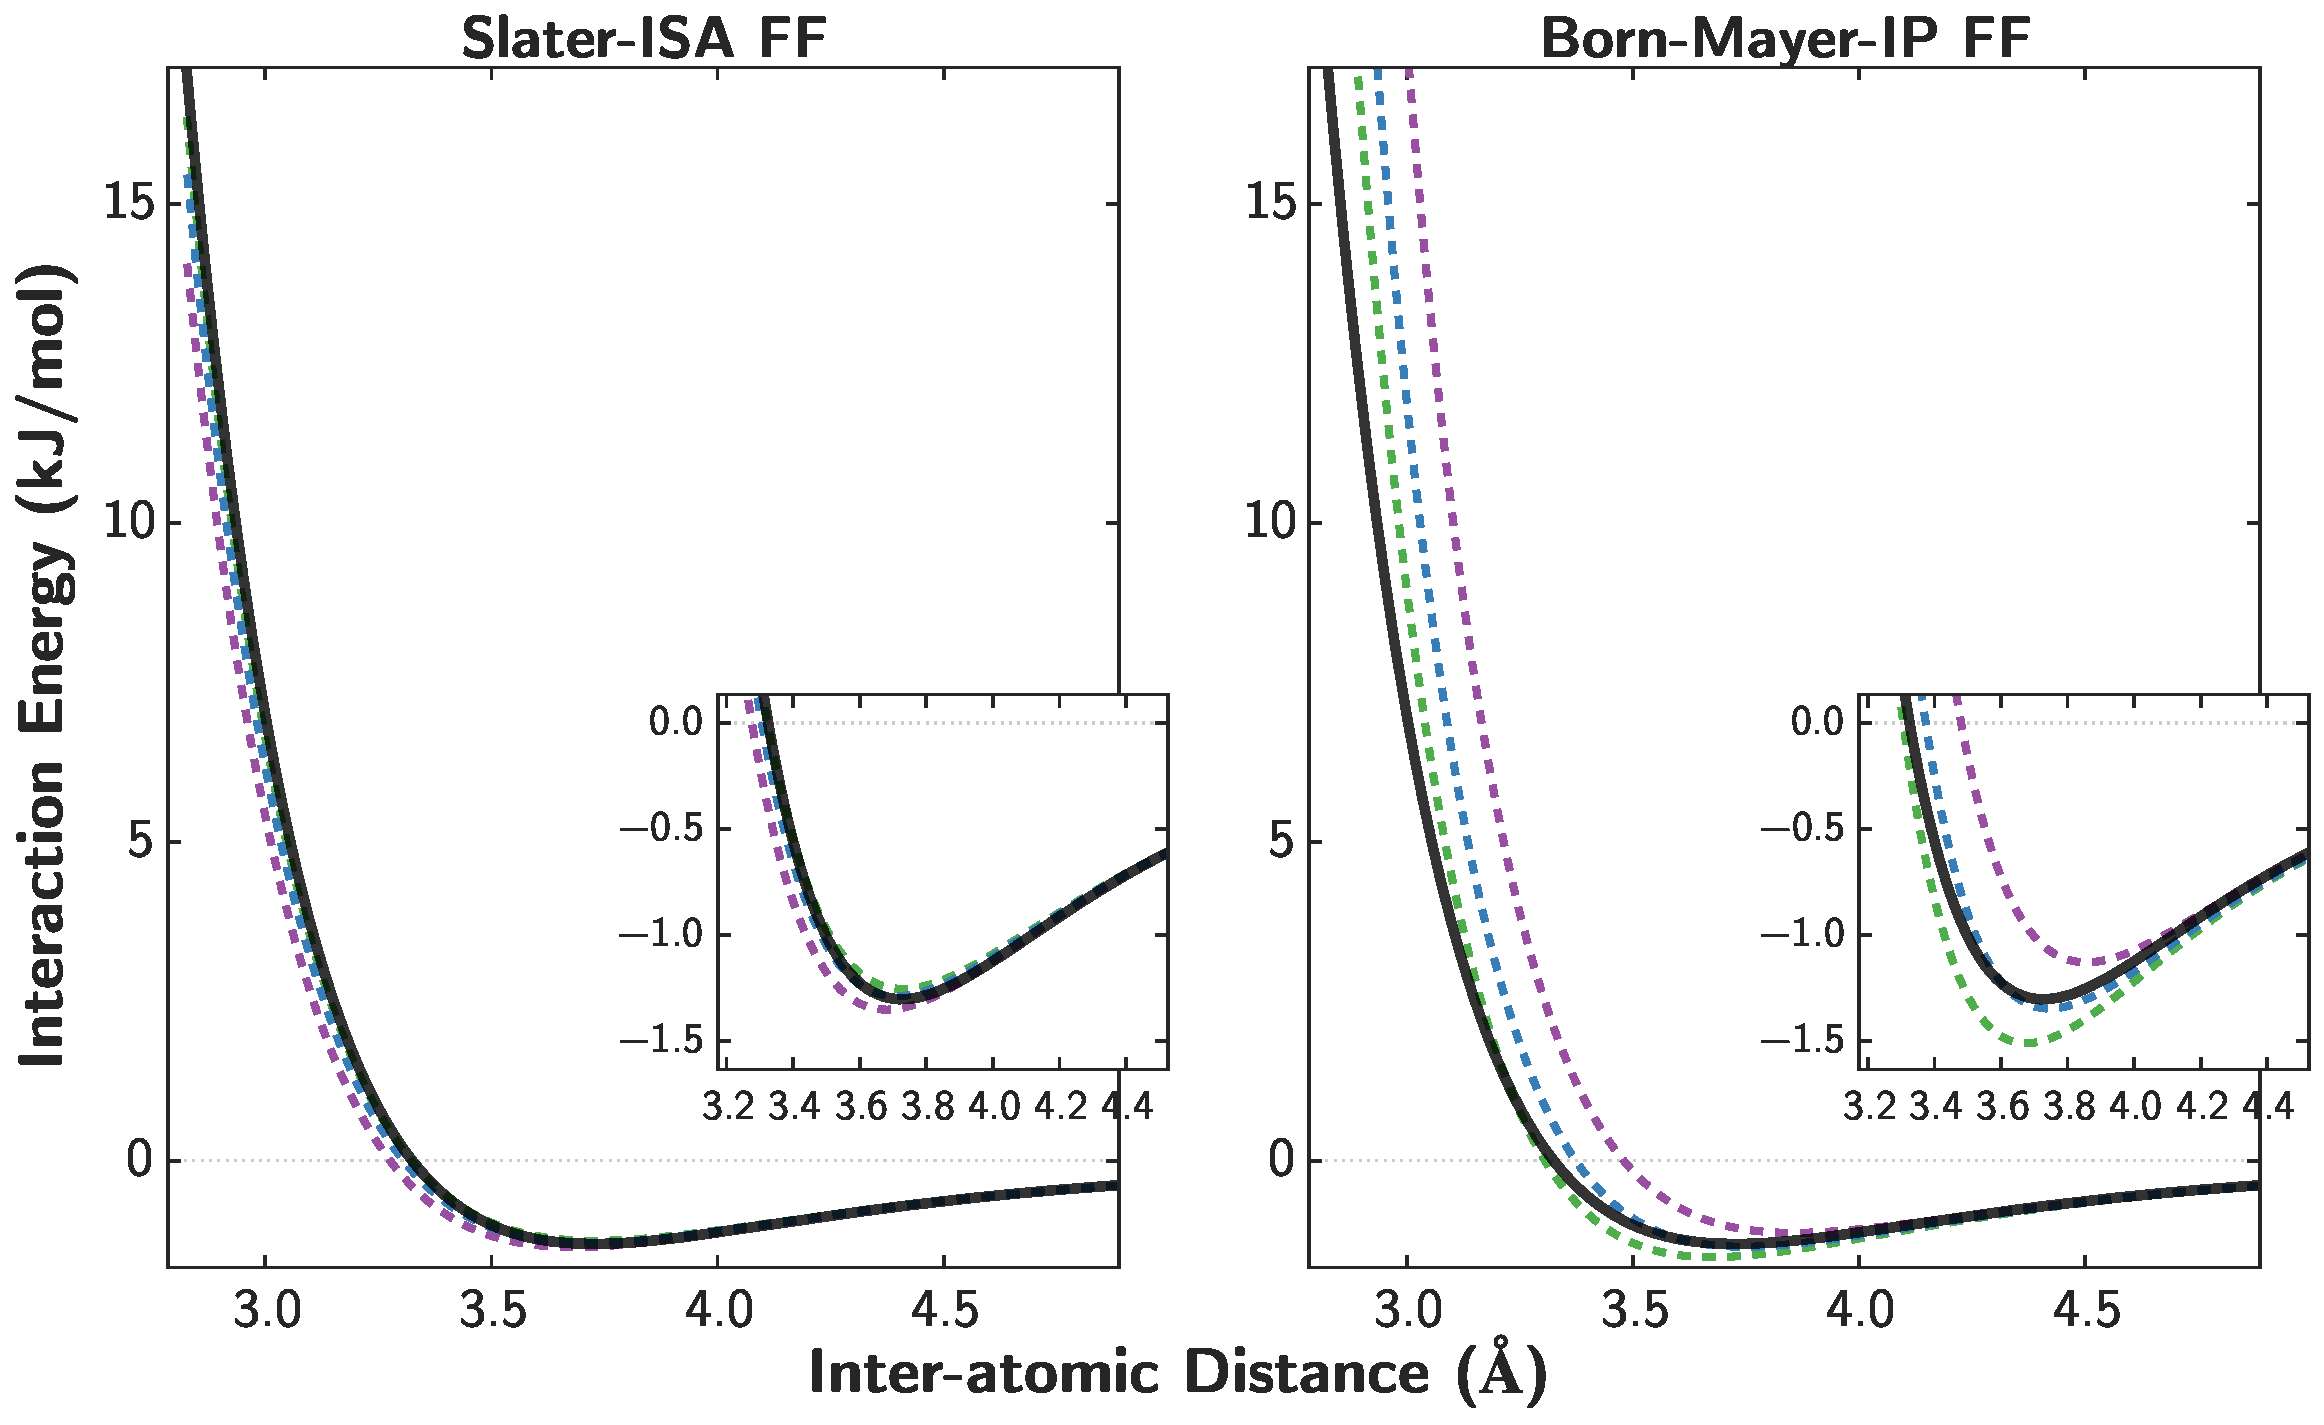
\includegraphics[width=0.8\textwidth]{isotropic/si/compare_ar_ar_scan.pdf}
%%     \vspace{10 mm}
%%     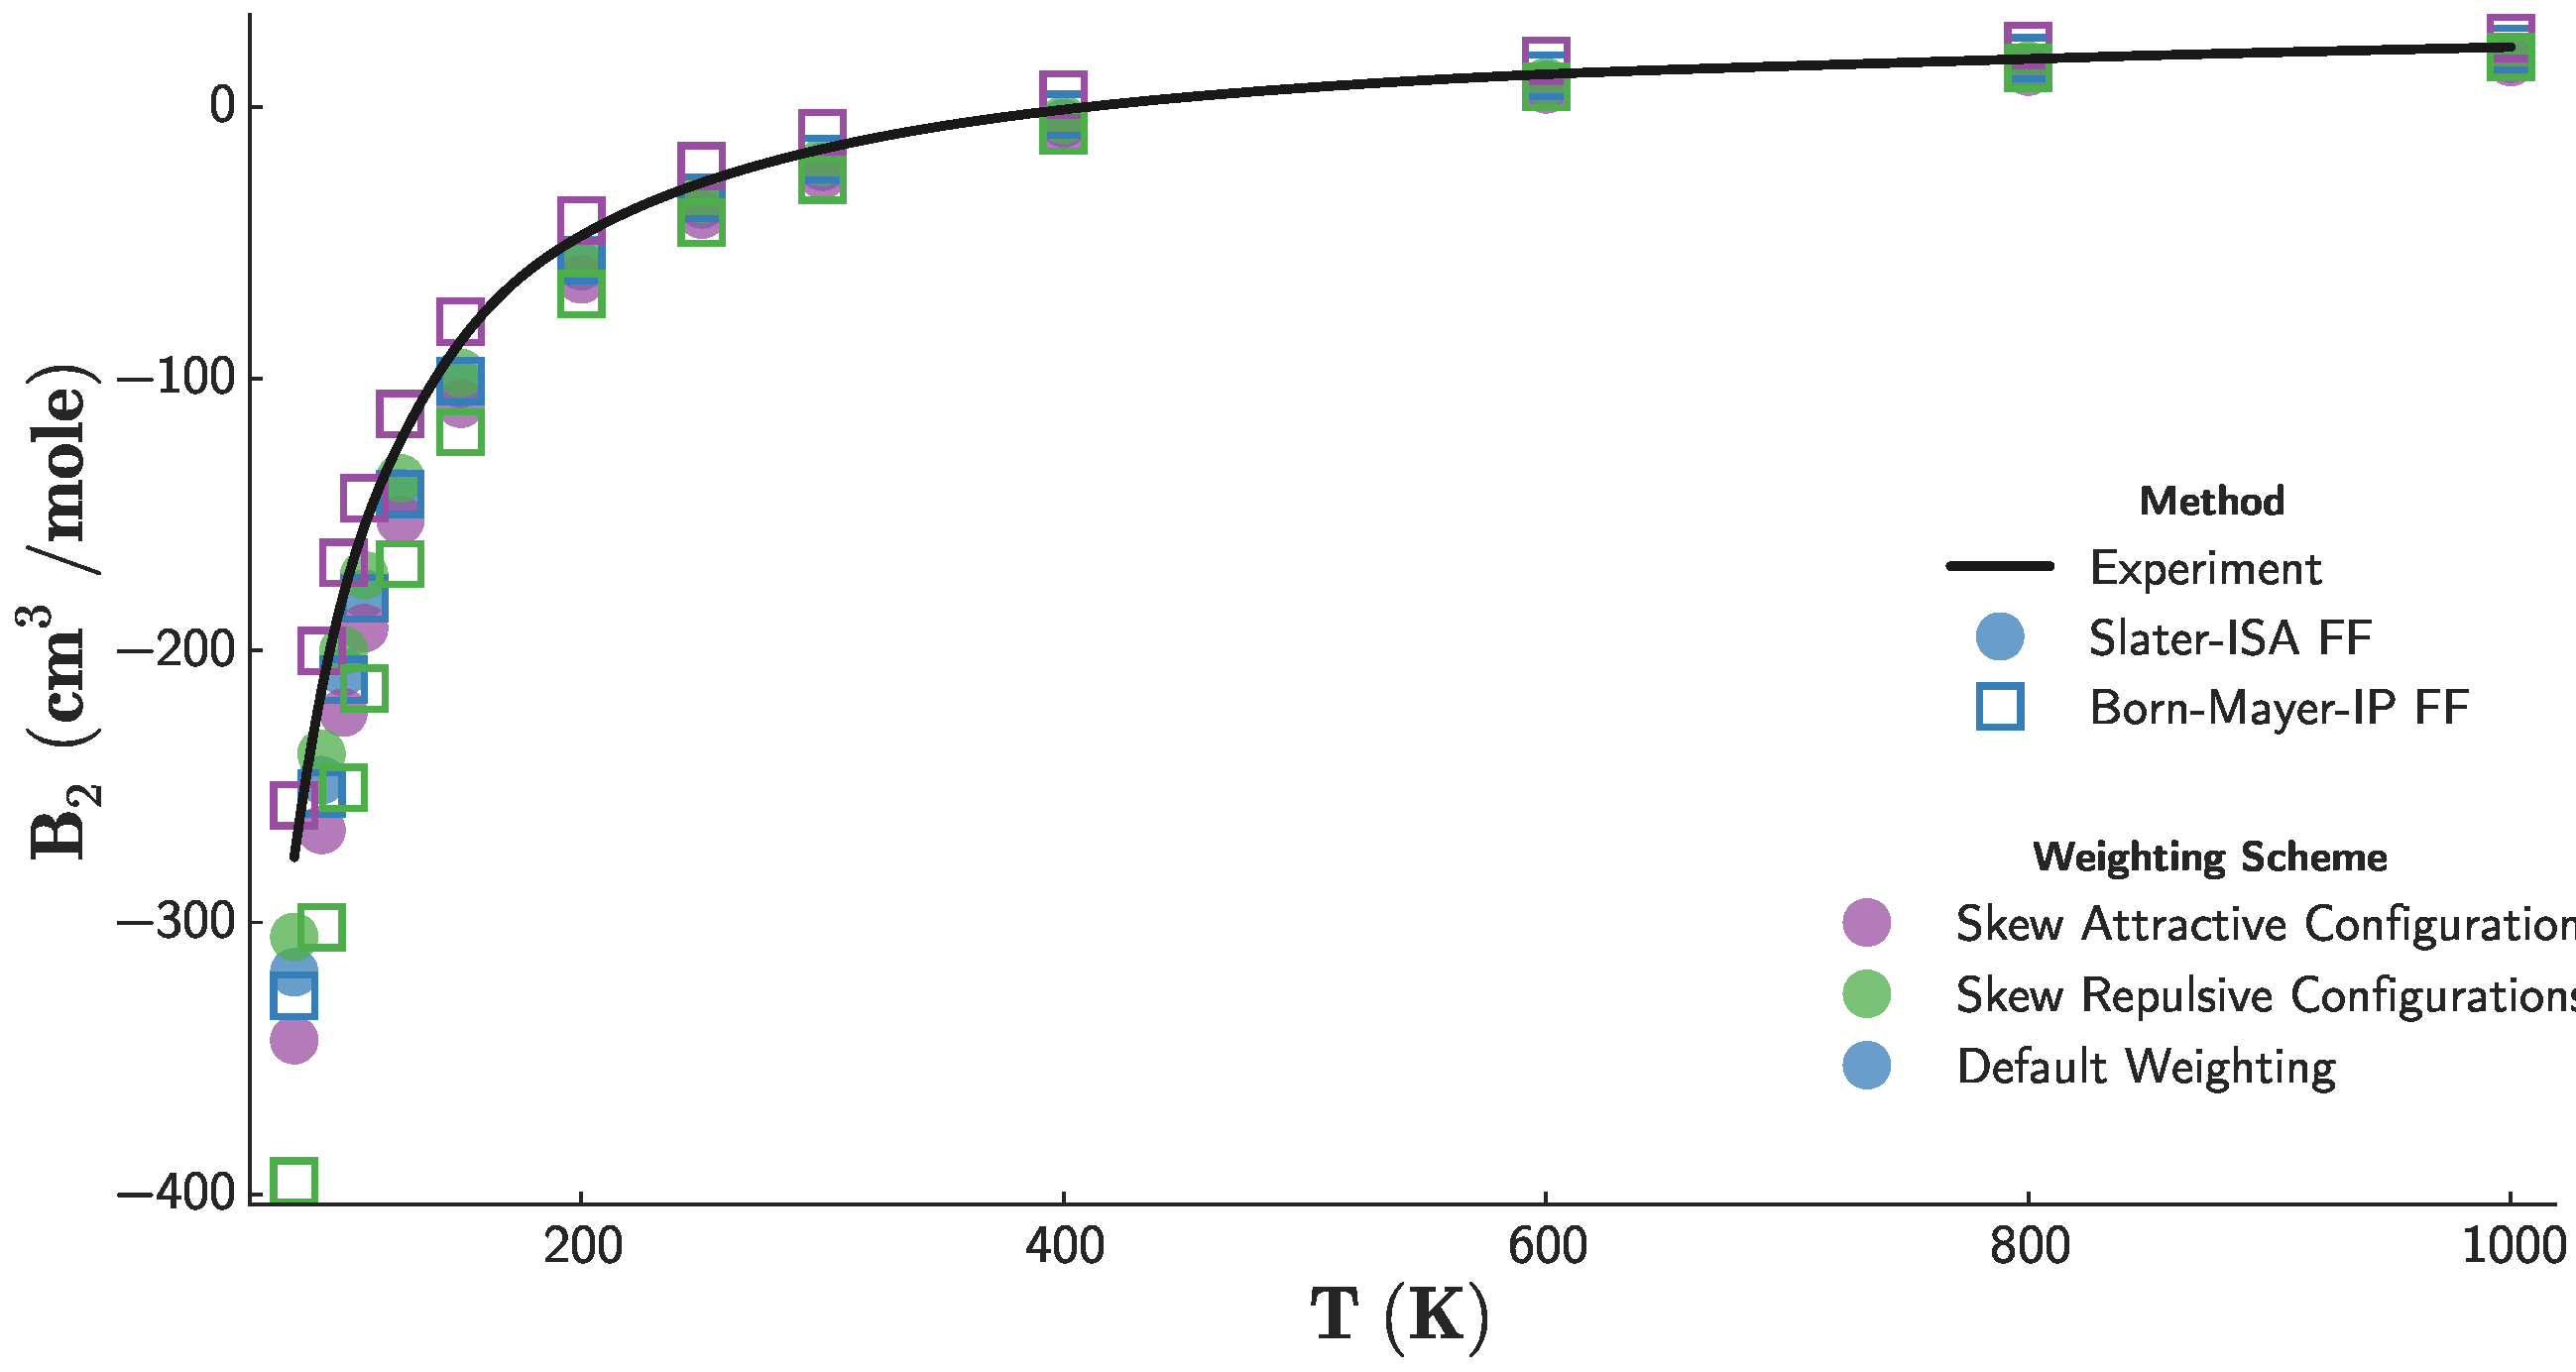
\includegraphics[width=0.8\textwidth]{isotropic/si/weighted_ar_2nd_virial.pdf}
%%     \caption[foo]{
%%         Comparison of the \isaffold and the \saptff in terms of sensitivity to the
%%         weighting function employed in parameter optimization for the Ar 
%%         dimer. Three weighting functions, $\lambda = 0.5$ (purple), $\lambda = 2.0$
%%         (blue), and $\lambda = 5.0$ (green) are shown, with higher $\lambda$ values
%%         indicating more weighting of repulsive configurations.
%%               
%%         (top) Total interaction energies for the \isaffold (left) and the \saptff (right)
%%         indicating the accuracy of each force field with respect to \saptpbeo benchmark
%%         energies. DFT-SAPT energies are shown as black solid lines, force field fits with
%%         dotted lines. Colors for the different weighting functions is as above.
%%               
%%         (bottom) Computed 2$^\text{nd}$ virial coefficients for argon. Data for
%%         the \isaffold and \saptff are depicted using open circles and shaded squares,
%%         respectively; coloration for the different weighting functions is as above.
%%         Experimental data from \citeauthor{Dymond1980} (black line) is also shown.
%%       %ASK: Do we actually cite Dymond and Smith for this, since it's a compiled
%%       %work, or do I need to try and dig up the original experimentallist?
%%     }
%%     \label{fig:ar-weighting}
%% 
%%     \end{figure}
%%     %%%%%%%% Weighting Function Tests %%%%%%%
%% 
%% \end{section}
%% 
%% 
%% \clearpage
%% \begin{section}{Parameter Robustness for Ethane; \ljff results}
%% 
%% 
%% Ethane parameters were tested for robustness by changing the weighting function
%% as described in the main text. Optimized \isaffold \A parameters are
%% much less sensitive to the choice of weighting function compared to
%% the \ljff. As a result, the \isaffold shows decreased uncertainty when computing
%% the 2\super{nd} virial coefficient. Virial coefficients for the \ljff, on the
%% other hand, depend more strongly on the choice of weighting function. 
%% 
%% 
%%     %%%%%%%% Weighting Function Tests %%%%%%%
%%     \begin{figure}
%%     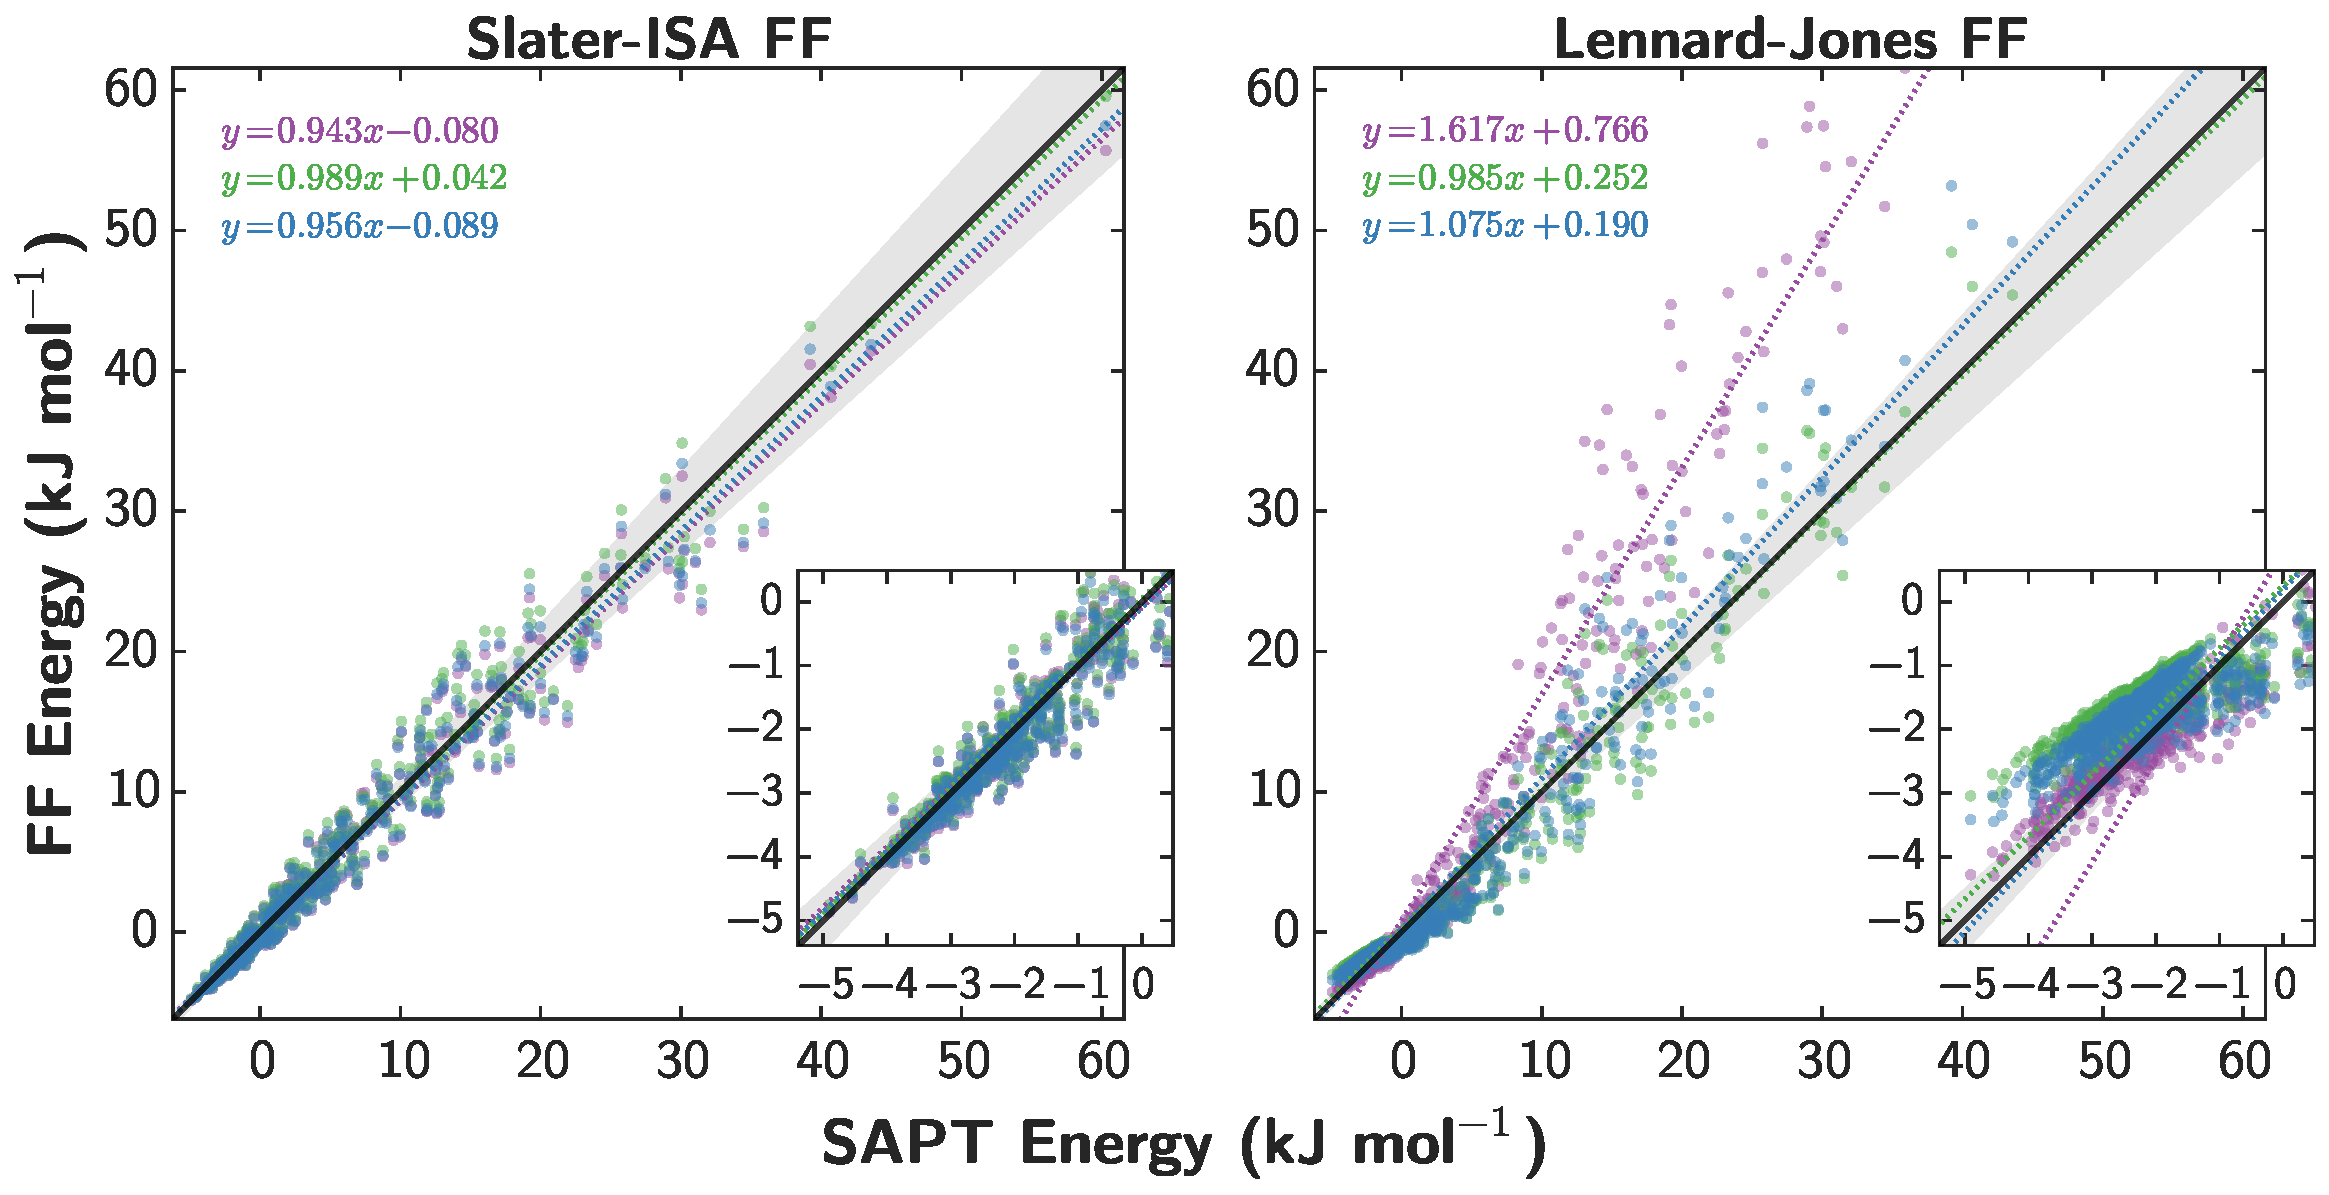
\includegraphics[width=0.8\textwidth]{isotropic/si/compare_lj_ethane_ethane_scatter.pdf}
%%     \vspace{10 mm}
%%     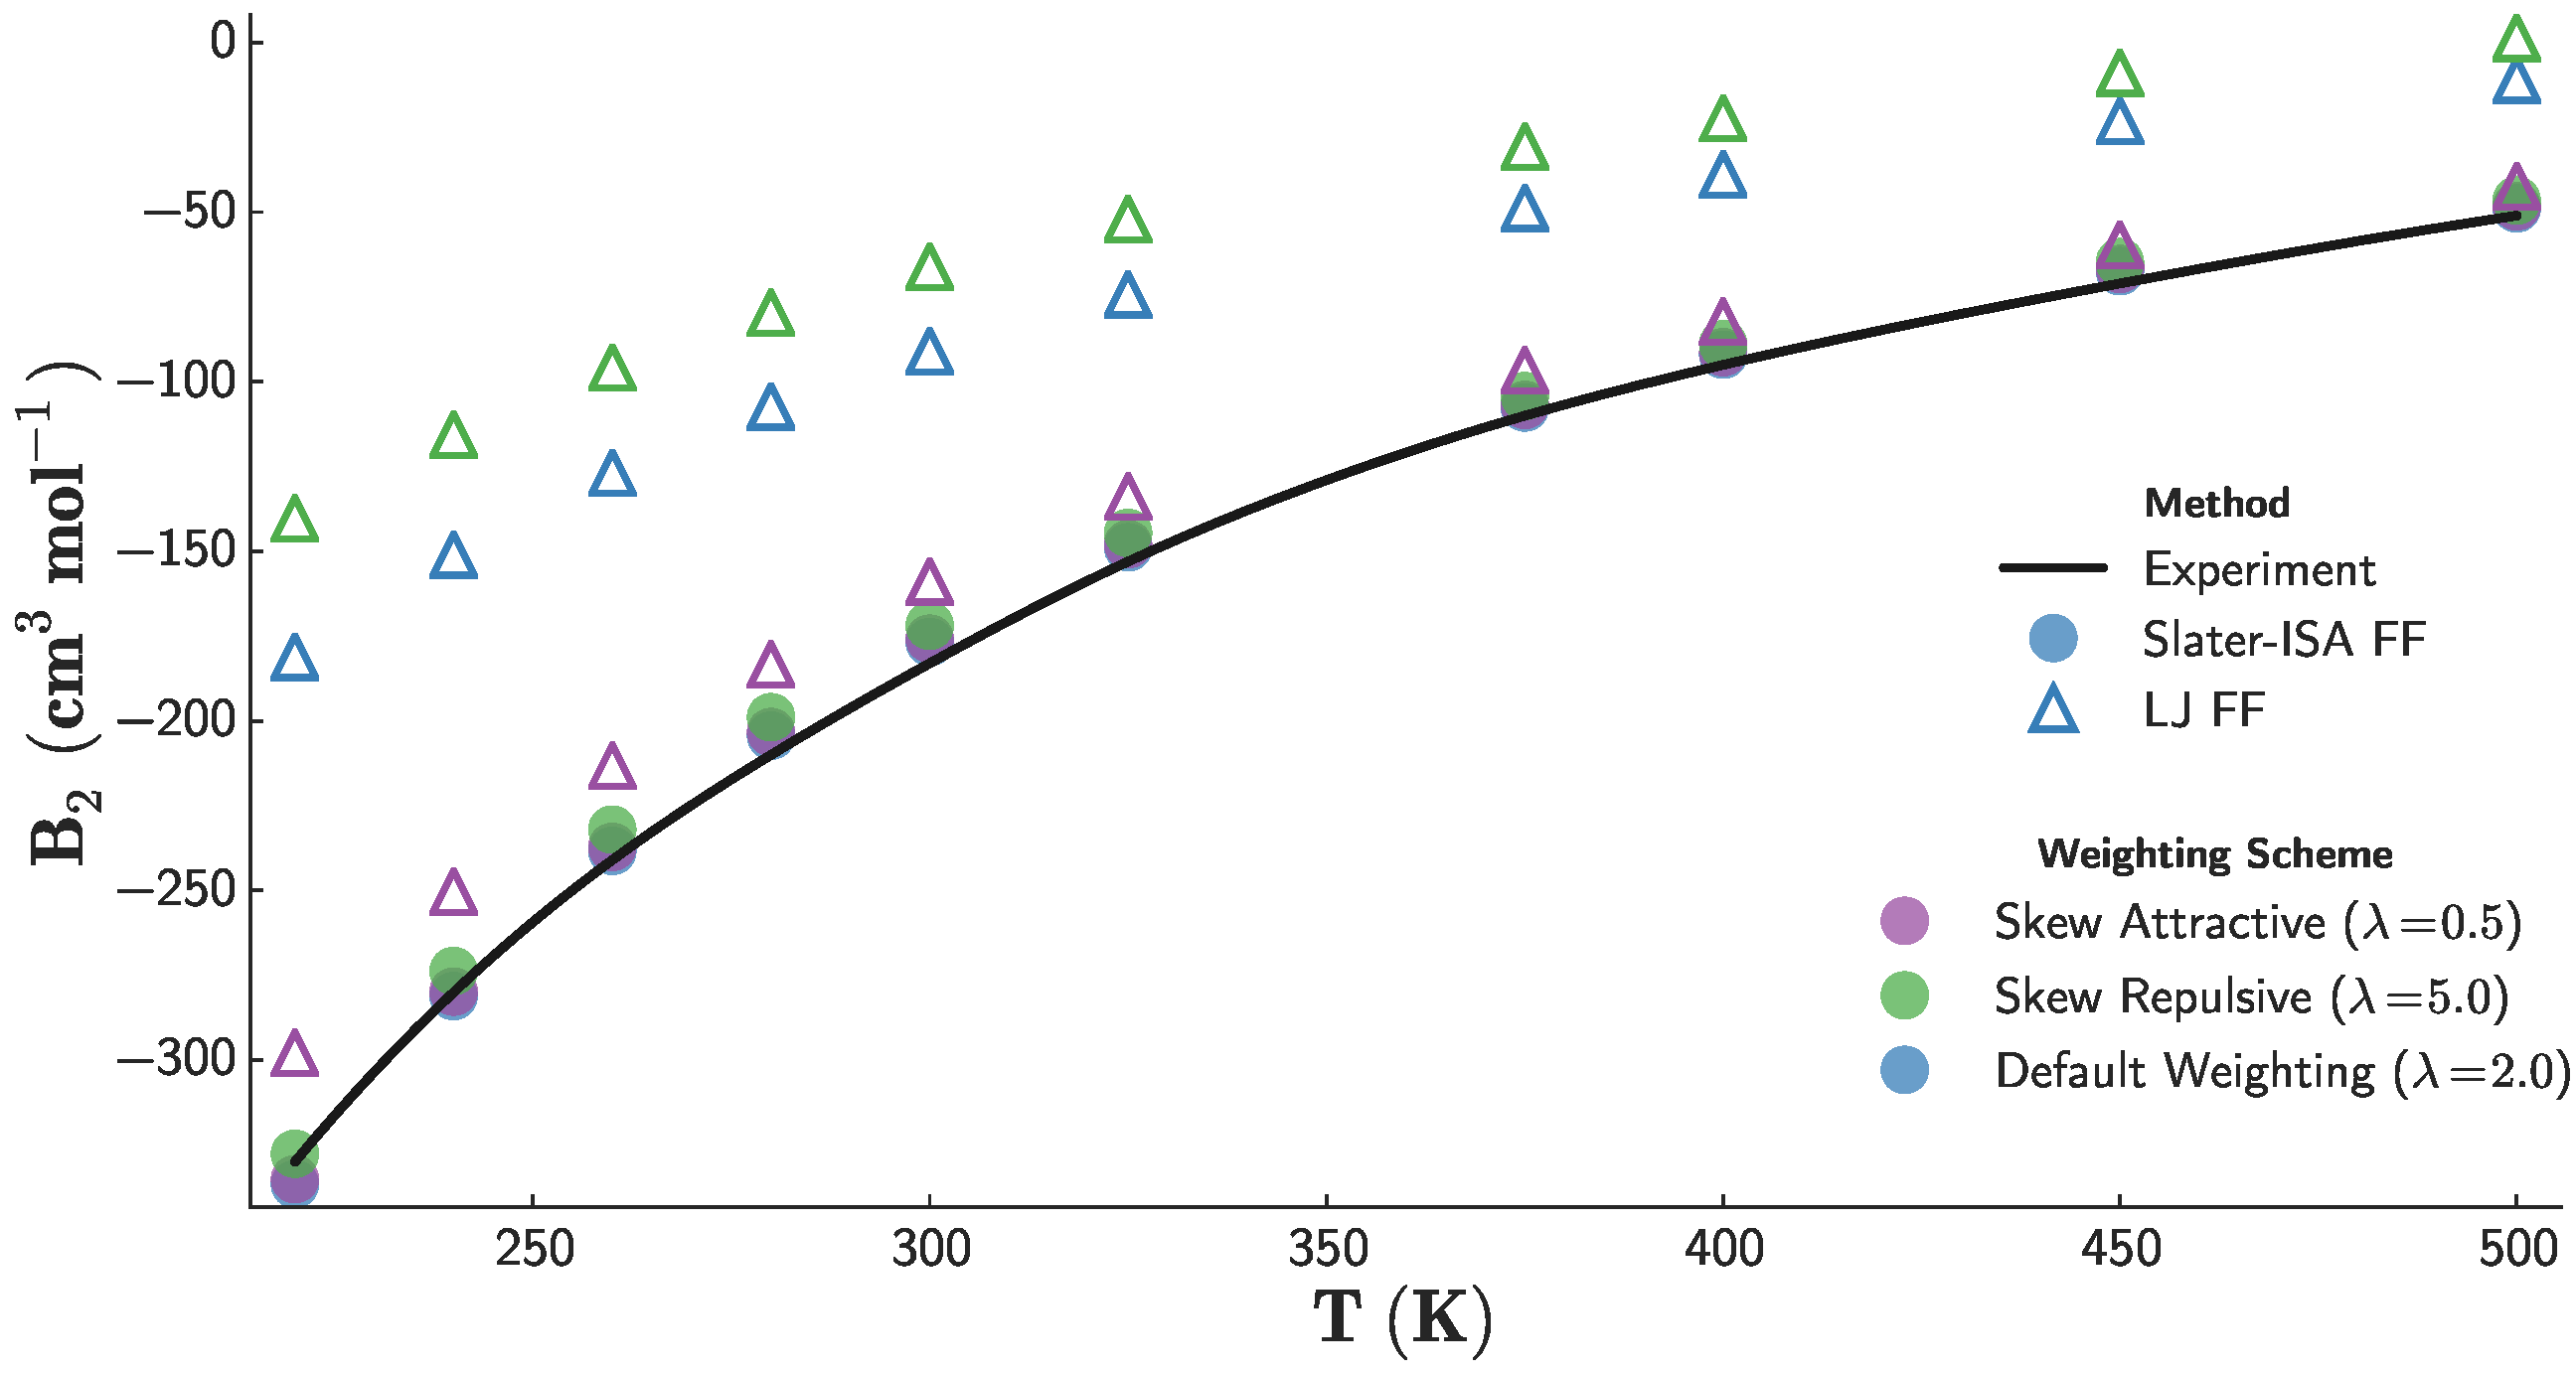
\includegraphics[width=0.8\textwidth]{isotropic/si/weighted_ethane_2nd_virial_lj.pdf}
%%     \caption[foo]{
%%         Comparison of the \isaffold and the \ljff in terms of sensitivity to the
%%         weighting function employed in parameter optimization for the ethane
%%         dimer. Three weighting functions, $\lambda = 0.5$ (purple), $\lambda = 2.0$
%%         (blue), and $\lambda = 5.0$ (green) are shown, with higher $\lambda$ values
%%         indicating more weighting of repulsive configurations.
%% 
%%         (top) Total interaction energies for the \isaffold (left) and the \ljff (right)
%%         indicating the accuracy of each force field with respect to \saptpbeo benchmark
%%         energies.  The diagonal line (black) indicates perfect agreement between
%%         reference energies and each force field, while shaded grey areas represent
%%         points within $\pm 10\%$ agreement of the benchmark.  To guide the eye, a line
%%         of best fit (dotted line) has been computed for each force field and for each
%%         weighting function.
%%               
%%         (bottom) Computed 2$^\text{nd}$ virial coefficients for argon. Data for
%%         the \isaffold and the \saptff are depicted using open circles and shaded squares,
%%         respectively; coloration for the different weighting functions is as above.
%%         Experimental data from \citeauthor{Dymond1980} (black line) is also shown.
%%       %ASK: Do we actually cite Dymond and Smith for this, since it's a compiled
%%       %work, or do I need to try and dig up the original experimentallist?
%%     }
%%     \label{fig:ar-weighting}
%% 
%%     \end{figure}
%%     %%%%%%%% Weighting Function Tests %%%%%%%
%% \end{section}
%% 
%% 
%% \pagebreak
%% \scriptsize
%% %% \begin{table}
\centering
\renewcommand\arraystretch{1.1}
\begin{longtable}{@{}ccccccc@{}}
\caption{Fitted values for Bij for a variety of element pairs. All values are
given in atomic units, except for RMS errors, which are a unitless normalized
overlap.} \label{tab:all_bij_exponents} \\

\hline
\toprule
$i$ &  $j$  &        $B_i$     &     $B_j$     &    $B_{ij}$   &      RMSE   & MAPE   \\    
\midrule
\endfirsthead

\multicolumn{6}{c}%
{{\bfseries \tablename\ \thetable{} -- continued from previous page}} \\
\hline
\toprule
$i$ &  $j$  &        $B_i$     &     $B_j$     &    $B_{ij}$   &      RMSE  & MAPE    \\    
\midrule
\endhead

\bottomrule
\hline
\endfoot

H  &  He    &     1.99946394   &   2.68859863  &    2.31740474 &  0.00044277657  &  0.882930\\
H  &  Li    &     1.99946394   &   1.25901971  &    1.59404909 &  0.00064319203  &  1.106033\\
H  &  Be    &     1.99946394   &   1.65554322  &    1.82052039 &  0.00012960395  &  0.217206\\
H  &  B     &     1.99946394   &   1.56191136  &    1.76768239 &  0.00022762336  &  0.498291\\
H  &  C     &     1.99946394   &   1.81946896  &    1.90742066 &  3.6383389e-05  &  0.074853\\
H  &  N     &     1.99946394   &   2.06711073  &    2.03302187 &  4.9406068e-06  &  0.009742\\
H  &  O     &     1.99946394   &   2.00091172  &    2.00019722 &  9.9506754e-08  &  0.000183\\
H  &  F     &     1.99946394   &   2.26322976  &    2.12730789 &  7.0666272e-05  &  0.137228\\
H  &  Ne    &     1.99946394   &   2.51791099  &    2.24270366 &  0.00026455338  &  0.578093\\
H  &  Na    &     1.99946394   &   1.22917354  &    1.57023314 &  0.00074952732  &  1.738728\\
H  &  Mg    &     1.99946394   &   1.49931366  &    1.73354253 &   0.0002881065  &  0.529739\\
H  &  Al    &     1.99946394   &   1.32657183  &    1.63349076 &  0.00053449852  &  0.976877\\
H  &  Si    &     1.99946394   &   1.54808130  &    1.75910683 &  0.00024917876  &  0.617006\\
H  &  P     &     1.99946394   &   1.75585679  &    1.87377325 &  6.8182489e-05  &  0.148197\\
H  &  S     &     1.99946394   &   1.74521745  &    1.86810662 &  7.4332699e-05  &  0.160880\\
H  &  Cl    &     1.99946394   &   1.95253790  &    1.97586738 &  2.5436846e-06  &  0.005705\\
H  &  Ar    &     1.99946394   &   2.15249556  &    2.07440522 &  2.5899665e-05  &  0.068500\\
H  &  Br    &     1.99946394   &   1.86365053  &    1.93033996 &   2.112332e-05  &  0.048965\\
H  &  I     &     1.99946394   &   1.75289066  &    1.87194355 &  7.1892596e-05  &  0.178949\\
He &  Li    &     2.68859863   &   1.25901971  &    1.83579487 &   0.0020586815  &  4.802329\\
He &  Be    &     2.68859863   &   1.65554322  &    2.10352673 &   0.0010603604  &  2.573450\\
He &  B     &     2.68859863   &   1.56191136  &    2.03442611 &     0.00129508  &  3.918107\\
He &  C     &     2.68859863   &   1.81946896  &    2.20238570 &  0.00075763278  &  2.262394\\
He &  N     &     2.68859863   &   2.06711073  &    2.35237454 &   0.0003780889  &  1.127971\\
He &  O     &     2.68859863   &   2.00091172  &    2.31393264 &  0.00046386026  &  1.314845\\
He &  F     &     2.68859863   &   2.26322976  &    2.46423057 &   0.0001731239  &  0.522637\\
He &  Ne    &     2.68859863   &   2.51791099  &    2.60133215 &  2.7253815e-05  &  0.094670\\
He &  Na    &     2.68859863   &   1.22917354  &    1.79792813 &   0.0021797532  &  6.560866\\
He &  Mg    &     2.68859863   &   1.49931366  &    1.99849093 &   0.0014277708  &  3.668547\\
He &  Al    &     2.68859863   &   1.32657183  &    1.88040364 &   0.0018777097  &  4.668027\\
He &  Si    &     2.68859863   &   1.54808130  &    2.02089719 &    0.001334628  &  4.489483\\
He &  P     &     2.68859863   &   1.75585679  &    2.16119527 &  0.00087958401  &  2.730605\\
He &  S     &     2.68859863   &   1.74521745  &    2.15451616 &  0.00090006465  &  2.778815\\
He &  Cl    &     2.68859863   &   1.95253790  &    2.28271739 &  0.00054130424  &  1.785225\\
He &  Ar    &     2.68859863   &   2.15249556  &    2.39953728 &  0.00028412395  &  1.122892\\
He &  Br    &     2.68859863   &   1.86365053  &    2.22767127 &  0.00068597032  &  2.295912\\
He &  I     &     2.68859863   &   1.75289066  &    2.15618545 &      0.0008917  &  3.122234\\
Li &  Be    &     1.25901971   &   1.65554322  &    1.44552618 &  0.00021566494  &  0.459735\\
Li &  B     &     1.25901971   &   1.56191136  &    1.40276036 &  0.00013669061  &  0.361720\\
Li &  C     &     1.25901971   &   1.81946896  &    1.51465672 &  0.00042489929  &  1.056460\\
Li &  N     &     1.25901971   &   2.06711073  &    1.61476325 &  0.00080816618  &  1.922263\\
Li &  O     &     1.25901971   &   2.00091172  &    1.58945583 &  0.00069142836  &  1.593136\\
Li &  F     &     1.25901971   &   2.26322976  &    1.68919749 &   0.0011668895  &  2.718352\\
Li &  Ne    &     1.25901971   &   2.51791099  &    1.77555429 &   0.0017026265  &  4.273871\\
Li &  Na    &     1.25901971   &   1.22917354  &    1.24402068 &  1.5533688e-06  &  0.004373\\
Li &  Mg    &     1.25901971   &   1.49931366  &    1.37457277 &  8.4735331e-05  &  0.195212\\
Li &  Al    &     1.25901971   &   1.32657183  &    1.29242716 &  7.1019258e-06  &  0.016335\\
Li &  Si    &     1.25901971   &   1.54808130  &    1.39618447 &  0.00012793291  &  0.374607\\
Li &  P     &     1.25901971   &   1.75585679  &    1.48750641 &  0.00034426274  &  0.896554\\
Li &  S     &     1.25901971   &   1.74521745  &    1.48302253 &  0.00033062213  &  0.858653\\
Li &  Cl    &     1.25901971   &   1.95253790  &    1.56786800 &  0.00063028803  &  1.664314\\
Li &  Ar    &     1.25901971   &   2.15249556  &    1.64158799 &  0.00099309611  &  2.932927\\
Li &  Br    &     1.25901971   &   1.86365053  &    1.53172970 &  0.00049638053  &  1.350986\\
Li &  I     &     1.25901971   &   1.75289066  &    1.48527643 &  0.00034799167  &  1.009017\\
Be &  B     &     1.65554322   &   1.56191136  &    1.60804807 &  1.1972231e-05  &  0.031893\\
Be &  C     &     1.65554322   &   1.81946896  &    1.73554580 &  3.3972736e-05  &  0.085743\\
Be &  N     &     1.65554322   &   2.06711073  &    1.84956812 &   0.0001992019  &  0.484038\\
Be &  O     &     1.65554322   &   2.00091172  &    1.82001716 &  0.00014155775  &  0.330806\\
Be &  F     &     1.65554322   &   2.26322976  &    1.93457449 &  0.00041123838  &  0.983581\\
Be &  Ne    &     1.65554322   &   2.51791099  &    2.03628351 &  0.00078343308  &  2.059895\\
Be &  Na    &     1.65554322   &   1.22917354  &    1.42686604 &  0.00026737271  &  0.745777\\
Be &  Mg    &     1.65554322   &   1.49931366  &    1.57563633 &  3.2478195e-05  &  0.074055\\
Be &  Al    &     1.65554322   &   1.32657183  &    1.48286105 &  0.00014866739  &  0.335525\\
Be &  Si    &     1.65554322   &   1.54808130  &    1.60086762 &   1.615263e-05  &  0.048036\\
Be &  P     &     1.65554322   &   1.75585679  &    1.70494709 &  1.3101092e-05  &  0.034696\\
Be &  S     &     1.65554322   &   1.74521745  &    1.69977980 &  1.0504303e-05  &  0.027715\\
Be &  Cl    &     1.65554322   &   1.95253790  &    1.79750301 &  0.00010922498  &  0.297117\\
Be &  Ar    &     1.65554322   &   2.15249556  &    1.88512628 &  0.00029576275  &  0.923403\\
Be &  Br    &     1.65554322   &   1.86365053  &    1.75630627 &  5.5219463e-05  &  0.154638\\
Be &  I     &     1.65554322   &   1.75289066  &    1.70346914 &  1.2636043e-05  &  0.037713\\
B  &  C     &     1.56191136   &   1.81946896  &    1.68526246 &   8.896852e-05  &  0.279460\\
B  &  N     &     1.56191136   &   2.06711073  &    1.79465183 &  0.00031660316  &  0.962841\\
B  &  O     &     1.56191136   &   2.00091172  &    1.76649990 &  0.00024246047  &  0.712022\\
B  &  F     &     1.56191136   &   2.26322976  &    1.87554766 &  0.00057369687  &  1.719903\\
B  &  Ne    &     1.56191136   &   2.51791099  &    1.97105959 &  0.00099084843  &  3.222525\\
B  &  Na    &     1.56191136   &   1.22917354  &    1.38509763 &  0.00017473338  &  0.590078\\
B  &  Mg    &     1.56191136   &   1.49931366  &    1.53029477 &  5.6807294e-06  &  0.016154\\
B  &  Al    &     1.56191136   &   1.32657183  &    1.43954012 &  8.2359665e-05  &  0.230371\\
B  &  Si    &     1.56191136   &   1.54808130  &    1.55498504 &  3.4970147e-07  &  0.001260\\
B  &  P     &     1.56191136   &   1.75585679  &    1.65571982 &  5.1764703e-05  &  0.169673\\
B  &  S     &     1.56191136   &   1.74521745  &    1.65073751 &  4.6359978e-05  &  0.151426\\
B  &  Cl    &     1.56191136   &   1.95253790  &    1.74462228 &  0.00019882685  &  0.668654\\
B  &  Ar    &     1.56191136   &   2.15249556  &    1.82774537 &  0.00043254436  &  1.644894\\
B  &  Br    &     1.56191136   &   1.86365053  &    1.70507656 &  0.00012232055  &  0.422076\\
B  &  I     &     1.56191136   &   1.75289066  &    1.65418604 &  5.1089297e-05  &  0.186574\\
C  &  N     &     1.81946896   &   2.06711073  &    1.93878424 &  7.2588349e-05  &  0.213967\\
C  &  O     &     1.81946896   &   2.00091172  &    1.90779431 &  3.9381872e-05  &  0.111509\\
C  &  F     &     1.81946896   &   2.26322976  &    2.02729827 &  0.00022128603  &  0.646349\\
C  &  Ne    &     1.81946896   &   2.51791099  &    2.13356824 &  0.00051712548  &  1.665041\\
C  &  Na    &     1.81946896   &   1.22917354  &    1.49359005 &  0.00049650546  &  1.590315\\
C  &  Mg    &     1.81946896   &   1.49931366  &    1.65145683 &  0.00013523926  &  0.364498\\
C  &  Al    &     1.81946896   &   1.32657183  &    1.55375705 &  0.00032909645  &  0.868090\\
C  &  Si    &     1.81946896   &   1.54808130  &    1.67745495 &  0.00010070423  &  0.351275\\
C  &  P     &     1.81946896   &   1.75585679  &    1.78734889 &  5.2847945e-06  &  0.016690\\
C  &  S     &     1.81946896   &   1.74521745  &    1.78191233 &  7.1848878e-06  &  0.022600\\
C  &  Cl    &     1.81946896   &   1.95253790  &    1.88462580 &  2.1955555e-05  &  0.071858\\
C  &  Ar    &     1.81946896   &   2.15249556  &    1.97704725 &   0.0001323859  &  0.499304\\
C  &  Br    &     1.81946896   &   1.86365053  &    1.84141110 &  2.5492317e-06  &  0.008538\\
C  &  I     &     1.81946896   &   1.75289066  &    1.78581710 &  5.8824253e-06  &  0.020847\\
N  &  O     &     2.06711073   &   2.00091172  &    2.03371451 &   5.041231e-06  &  0.013929\\
N  &  F     &     2.06711073   &   2.26322976  &    2.16254689 &    4.15042e-05  &  0.119485\\
N  &  Ne    &     2.06711073   &   2.51791099  &    2.27840189 &  0.00020910088  &  0.673215\\
N  &  Na    &     2.06711073   &   1.22917354  &    1.58958212 &  0.00090815621  &  2.796799\\
N  &  Mg    &     2.06711073   &   1.49931366  &    1.75954426 &  0.00039310972  &  1.019328\\
N  &  Al    &     2.06711073   &   1.32657183  &    1.65570661 &  0.00068105488  &  1.722447\\
N  &  Si    &     2.06711073   &   1.54808130  &    1.78559923 &  0.00033982883  &  1.150687\\
N  &  P     &     2.06711073   &   1.75585679  &    1.90415582 &  0.00011669305  &  0.359120\\
N  &  S     &     2.06711073   &   1.74521745  &    1.89832775 &  0.00012494822  &  0.382742\\
N  &  Cl    &     2.06711073   &   1.95253790  &    2.00885032 &  1.5404889e-05  &  0.049510\\
N  &  Ar    &     2.06711073   &   2.15249556  &    2.10924579 &  8.3837241e-06  &  0.031515\\
N  &  Br    &     2.06711073   &   1.86365053  &    1.96222048 &   4.938888e-05  &  0.162281\\
N  &  I     &     2.06711073   &   1.75289066  &    1.90214169 &  0.00012093134  &  0.419448\\
O  &  F     &     2.00091172   &   2.26322976  &    2.12742019 &  7.4513608e-05  &  0.204667\\
O  &  Ne    &     2.00091172   &   2.51791099  &    2.24105845 &  0.00027602296  &  0.845765\\
O  &  Na    &     2.00091172   &   1.22917354  &    1.56546880 &  0.00078625246  &  2.354990\\
O  &  Mg    &     2.00091172   &   1.49931366  &    1.73176044 &  0.00031061975  &  0.777382\\
O  &  Al    &     2.00091172   &   1.32657183  &    1.62980355 &  0.00057319586  &  1.403523\\
O  &  Si    &     2.00091172   &   1.54808130  &    1.75782981 &  0.00026287602  &  0.860753\\
O  &  P     &     2.00091172   &   1.75585679  &    1.87387688 &  7.3175089e-05  &  0.216650\\
O  &  S     &     2.00091172   &   1.74521745  &    1.86815729 &  7.9760452e-05  &  0.235090\\
O  &  Cl    &     2.00091172   &   1.95253790  &    1.97655937 &  2.8387158e-06  &  0.008742\\
O  &  Ar    &     2.00091172   &   2.15249556  &    2.07494432 &  2.6479263e-05  &  0.095246\\
O  &  Br    &     2.00091172   &   1.86365053  &    1.93085797 &  2.2760392e-05  &  0.071837\\
O  &  I     &     2.00091172   &   1.75289066  &    1.87203787 &  7.6356395e-05  &  0.255064\\
F  &  Ne    &     2.26322976   &   2.51791099  &    2.38617019 &  6.4967098e-05  &  0.211473\\
F  &  Na    &     2.26322976   &   1.22917354  &    1.66029149 &   0.0012830926  &  3.875179\\
F  &  Mg    &     2.26322976   &   1.49931366  &    1.83986590 &  0.00066962961  &  1.706670\\
F  &  Al    &     2.26322976   &   1.32657183  &    1.73140874 &   0.0010196712  &  2.528620\\
F  &  Si    &     2.26322976   &   1.54808130  &    1.86526151 &  0.00060490347  &  2.020578\\
F  &  P     &     2.26322976   &   1.75585679  &    1.99065290 &  0.00029360355  &  0.894671\\
F  &  S     &     2.26322976   &   1.74521745  &    1.98453998 &  0.00030630021  &  0.928727\\
F  &  Cl    &     2.26322976   &   1.95253790  &    2.10087150 &  0.00010755539  &  0.344316\\
F  &  Ar    &     2.26322976   &   2.15249556  &    2.20694293 &  1.3485721e-05  &  0.050987\\
F  &  Br    &     2.26322976   &   1.86365053  &    2.05158173 &  0.00018081195  &  0.590554\\
F  &  I     &     2.26322976   &   1.75289066  &    1.98794200 &  0.00030142935  &  1.036990\\
Ne &  Na    &     2.51791099   &   1.22917354  &    1.74146757 &   0.0018171227  &  5.842510\\
Ne &  Mg    &     2.51791099   &   1.49931366  &    1.93474540 &   0.0011134419  &  3.086201\\
Ne &  Al    &     2.51791099   &   1.32657183  &    1.81962923 &    0.001531155  &  4.095464\\
Ne &  Si    &     2.51791099   &   1.54808130  &    1.95888870 &   0.0010266525  &  3.702217\\
Ne &  P     &     2.51791099   &   1.75585679  &    2.09400464 &  0.00062146304  &  2.076964\\
Ne &  S     &     2.51791099   &   1.74521745  &    2.08750459 &  0.00063928574  &  2.124924\\
Ne &  Cl    &     2.51791099   &   1.95253790  &    2.21174754 &  0.00033656173  &  1.193911\\
Ne &  Ar    &     2.51791099   &   2.15249556  &    2.32497739 &  0.00013843693  &  0.584890\\
Ne &  Br    &     2.51791099   &   1.86365053  &    2.15873868 &      0.0004557  &  1.639505\\
Ne &  I     &     2.51791099   &   1.75289066  &    2.09004196 &  0.00063134274  &  2.372214\\
Na &  Mg    &     1.22917354   &   1.49931366  &    1.35766104 &  0.00011473889  &  0.341738\\
Na &  Al    &     1.22917354   &   1.32657183  &    1.27699602 &  1.5803838e-05  &  0.046721\\
Na &  Si    &     1.22917354   &   1.54808130  &    1.37861851 &  0.00016394224  &  0.606312\\
Na &  P     &     1.22917354   &   1.75585679  &    1.46734689 &  0.00040724885  &  1.358887\\
Na &  S     &     1.22917354   &   1.74521745  &    1.46301699 &  0.00039233117  &  1.305796\\
Na &  Cl    &     1.22917354   &   1.95253790  &    1.54462666 &  0.00071489747  &  2.415615\\
Na &  Ar    &     1.22917354   &   2.15249556  &    1.61475657 &   0.0010865392  &  4.048855\\
Na &  Br    &     1.22917354   &   1.86365053  &    1.50991318 &  0.00057095415  &  1.982122\\
Na &  I     &     1.22917354   &   1.75289066  &    1.46507909 &  0.00040898615  &  1.502211\\
Mg &  Al    &     1.49931366   &   1.32657183  &    1.41054381 &  4.3759475e-05  &  0.106460\\
Mg &  Si    &     1.49931366   &   1.54808130  &    1.52349731 &  3.5595022e-06  &  0.011234\\
Mg &  P     &     1.49931366   &   1.75585679  &    1.62233525 &  8.9250076e-05  &  0.251892\\
Mg &  S     &     1.49931366   &   1.74521745  &    1.61744114 &  8.2197924e-05  &  0.231214\\
Mg &  Cl    &     1.49931366   &   1.95253790  &    1.70986111 &  0.00026403315  &  0.761802\\
Mg &  Ar    &     1.49931366   &   2.15249556  &    1.79169870 &  0.00052474149  &  1.715332\\
Mg &  Br    &     1.49931366   &   1.86365053  &    1.67083027 &  0.00017608345  &  0.522795\\
Mg &  I     &     1.49931366   &   1.75289066  &    1.62071071 &  8.9123446e-05  &  0.281480\\
Al &  Si    &     1.32657183   &   1.54808130  &    1.43295795 &  7.4878405e-05  &  0.231698\\
Al &  P     &     1.32657183   &   1.75585679  &    1.52615042 &  0.00025709446  &  0.709802\\
Al &  S     &     1.32657183   &   1.74521745  &    1.52156219 &  0.00024519155  &  0.674974\\
Al &  Cl    &     1.32657183   &   1.95253790  &    1.60826232 &  0.00051441718  &  1.443233\\
Al &  Ar    &     1.32657183   &   2.15249556  &    1.68396084 &   0.0008502512  &  2.673094\\
Al &  Br    &     1.32657183   &   1.86365053  &    1.57145555 &  0.00039199648  &  1.132597\\
Al &  I     &     1.32657183   &   1.75289066  &    1.52414100 &  0.00025909364  &  0.796534\\
Si &  P     &     1.54808130   &   1.75585679  &    1.64816385 &  6.0537472e-05  &  0.219836\\
Si &  S     &     1.54808130   &   1.74521745  &    1.64322319 &  5.4646042e-05  &  0.197756\\
Si &  Cl    &     1.54808130   &   1.95253790  &    1.73616531 &  0.00021653004  &  0.806893\\
Si &  Ar    &     1.54808130   &   2.15249556  &    1.81809419 &  0.00045725342  &  1.916727\\
Si &  Br    &     1.54808130   &   1.86365053  &    1.69704848 &  0.00013598439  &  0.519161\\
Si &  I     &     1.54808130   &   1.75289066  &    1.64662155 &   5.971014e-05  &  0.240522\\
P  &  S     &     1.75585679   &   1.74521745  &    1.75053498 &  2.2383111e-07  &  0.000726\\
P  &  Cl    &     1.75585679   &   1.95253790  &    1.85109487 &  4.8767404e-05  &  0.166222\\
P  &  Ar    &     1.75585679   &   2.15249556  &    1.94118289 &  0.00019034099  &  0.743408\\
P  &  Br    &     1.75585679   &   1.86365053  &    1.80880477 &  1.5089803e-05  &  0.052666\\
P  &  I     &     1.75585679   &   1.75289066  &    1.75438024 &  8.3311914e-08  &  0.000297\\
S  &  Cl    &     1.74521745   &   1.95253790  &    1.84542979 &  5.4259063e-05  &  0.184109\\
S  &  Ar    &     1.74521745   &   2.15249556  &    1.93516069 &  0.00020092813  &  0.780785\\
S  &  Br    &     1.74521745   &   1.86365053  &    1.80328668 &  1.8231579e-05  &  0.063360\\
S  &  I     &     1.74521745   &   1.75289066  &    1.74905593 &  1.5042953e-07  &  0.000542\\
Cl &  Ar    &     1.95253790   &   2.15249556  &    2.04925011 &  4.7026489e-05  &  0.193758\\
Cl &  Br    &     1.95253790   &   1.86365053  &    1.90746100 &  9.8799774e-06  &  0.035850\\
Cl &  I     &     1.95253790   &   1.75289066  &    1.84935929 &  5.0999292e-05  &  0.194814\\
Ar &  Br    &     2.15249556   &   1.86365053  &    2.00111347 &  9.9755127e-05  &  0.417023\\
Ar &  I     &     2.15249556   &   1.75289066  &    1.93889388 &  0.00019497498  &  0.849907\\
Br &  I     &     1.86365053   &   1.75289066  &    1.80721936 &  1.6163908e-05  &  0.063089\\
%\bottomrule
\end{longtable}
%% \end{table}

%% \normalsize
%% 
%% %% \end{section}
%% 
%% 
%% \singlespacing
%% 
%% \renewcommand{\baselinestretch}{1}
%% 
%% \bibliographystyle{achemso}
%% \bibliography{/Users/Mary/Documents/library}
%% %\bibliography{rp_extras}
%% 
%% 
%% \end{document}
